%==============================================================================
% tento soubor pouzijte jako zaklad
% this file should be used as a base for the thesis
% Autoři / Authors: 2008 Michal Bidlo, 2019 Jaroslav Dytrych
% Kontakt pro dotazy a připomínky: sablona@fit.vutbr.cz
% Contact for questions and comments: sablona@fit.vutbr.cz
%==============================================================================
% kodovani: UTF-8 (zmena prikazem iconv, recode nebo cstocs)
% encoding: UTF-8 (you can change it by command iconv, recode or cstocs)
%------------------------------------------------------------------------------
% zpracování / processing: make, make pdf, make clean
%==============================================================================
% Soubory, které je nutné upravit nebo smazat: / Files which have to be edited or deleted:
%   projekt-20-literatura-bibliography.bib - literatura / bibliography
%   projekt-01-kapitoly-chapters.tex - obsah práce / the thesis content
%   projekt-01-kapitoly-chapters-en.tex - obsah práce v angličtině / the thesis content in English
%   projekt-30-prilohy-appendices.tex - přílohy / appendices
%   projekt-30-prilohy-appendices-en.tex - přílohy v angličtině / appendices in English
%==============================================================================
\documentclass[zadani]{fitthesis} % bez zadání - pro začátek práce, aby nebyl problém s překladem
%\documentclass[english]{fitthesis} % without assignment - for the work start to avoid compilation problem
%\documentclass[zadani]{fitthesis} % odevzdani do wisu a/nebo tisk s barevnými odkazy - odkazy jsou barevné
%\documentclass[english,zadani]{fitthesis} % for submission to the IS FIT and/or print with color links - links are color
%\documentclass[zadani,print]{fitthesis} % pro černobílý tisk - odkazy jsou černé
%\documentclass[english,zadani,print]{fitthesis} % for the black and white print - links are black
%\documentclass[zadani,cprint]{fitthesis} % pro barevný tisk - odkazy jsou černé, znak VUT barevný
%\documentclass[english,zadani,cprint]{fitthesis} % for the print - links are black, logo is color
% * Je-li práce psaná v anglickém jazyce, je zapotřebí u třídy použít 
%   parametr english následovně:
%   If thesis is written in English, it is necessary to use 
%   parameter english as follows:
%      \documentclass[english]{fitthesis}
% * Je-li práce psaná ve slovenském jazyce, je zapotřebí u třídy použít 
%   parametr slovak následovně:
%   If the work is written in the Slovak language, it is necessary 
%   to use parameter slovak as follows:
%      \documentclass[slovak]{fitthesis}
% * Je-li práce psaná v anglickém jazyce se slovenským abstraktem apod., 
%   je zapotřebí u třídy použít parametry english a enslovak následovně:
%   If the work is written in English with the Slovak abstract, etc., 
%   it is necessary to use parameters english and enslovak as follows:
%      \documentclass[english,enslovak]{fitthesis}

% Základní balíčky jsou dole v souboru šablony fitthesis.cls
% Basic packages are at the bottom of template file fitthesis.cls
% zde můžeme vložit vlastní balíčky / you can place own packages here

% Kompilace po částech (rychlejší, ale v náhledu nemusí být vše aktuální)
% Compilation piecewise (faster, but not all parts in preview will be up-to-date)
% \usepackage{subfiles}

% Nastavení cesty k obrázkům
% Setting of a path to the pictures
%\graphicspath{{obrazky-figures/}{./obrazky-figures/}}
%\graphicspath{{obrazky-figures/}{../obrazky-figures/}}

%---rm---------------
\renewcommand{\rmdefault}{lmr}%zavede Latin Modern Roman jako rm / set Latin Modern Roman as rm
%---sf---------------
\renewcommand{\sfdefault}{qhv}%zavede TeX Gyre Heros jako sf
%---tt------------
\renewcommand{\ttdefault}{lmtt}% zavede Latin Modern tt jako tt

% vypne funkci šablony, která automaticky nahrazuje uvozovky,
% aby nebyly prováděny nevhodné náhrady v popisech API apod.
% disables function of the template which replaces quotation marks
% to avoid unnecessary replacements in the API descriptions etc.
\csdoublequotesoff

\usepackage{url}
\usepackage{caption}

\usepackage{float}
\restylefloat{table}

% =======================================================================
% balíček "hyperref" vytváří klikací odkazy v pdf, pokud tedy použijeme pdflatex
% problém je, že balíček hyperref musí být uveden jako poslední, takže nemůže
% být v šabloně
% "hyperref" package create clickable links in pdf if you are using pdflatex.
% Problem is that this package have to be introduced as the last one so it 
% can not be placed in the template file.
\ifWis
\ifx\pdfoutput\undefined % nejedeme pod pdflatexem / we are not using pdflatex
\else
  \usepackage{color}
  \usepackage[unicode,colorlinks,hyperindex,plainpages=false,pdftex]{hyperref}
  \definecolor{hrcolor-ref}{RGB}{223,52,30}
  \definecolor{hrcolor-cite}{HTML}{2F8F00}
  \definecolor{hrcolor-urls}{HTML}{092EAB}
  \hypersetup{
	linkcolor=hrcolor-ref,
	citecolor=hrcolor-cite,
	filecolor=magenta,
	urlcolor=hrcolor-urls
  }
  \def\pdfBorderAttrs{/Border [0 0 0] }  % bez okrajů kolem odkazů / without margins around links
  \pdfcompresslevel=9
\fi
\else % pro tisk budou odkazy, na které se dá klikat, černé / for the print clickable links will be black
\ifx\pdfoutput\undefined % nejedeme pod pdflatexem / we are not using pdflatex
\else
  \usepackage{color}
  \usepackage[unicode,colorlinks,hyperindex,plainpages=false,pdftex,urlcolor=black,linkcolor=black,citecolor=black]{hyperref}
  \definecolor{links}{rgb}{0,0,0}
  \definecolor{anchors}{rgb}{0,0,0}
  \def\AnchorColor{anchors}
  \def\LinkColor{links}
  \def\pdfBorderAttrs{/Border [0 0 0] } % bez okrajů kolem odkazů / without margins around links
  \pdfcompresslevel=9
\fi
\fi
% Řešení problému, kdy klikací odkazy na obrázky vedou za obrázek
% This solves the problems with links which leads after the picture
\usepackage[all]{hypcap}

% Informace o práci/projektu / Information about the thesis
%---------------------------------------------------------------------------
\projectinfo{
  %Prace / Thesis
  project={BP},            %typ práce BP/SP/DP/DR  / thesis type (SP = term project)
  year={2021},             % rok odevzdání / year of submission
  date=\today,             % datum odevzdání / submission date
  %Nazev prace / thesis title
  title.cs={Strojové učení pro odpovídání na otázky v~přirozeném jazyce},  % název práce v češtině či slovenštině (dle zadání) / thesis title in czech language (according to assignment)
  title.en={Machine Learning for Natural Language Question Answering}, % název práce v angličtině / thesis title in english
  %title.length={14.5cm}, % nastavení délky bloku s titulkem pro úpravu zalomení řádku (lze definovat zde nebo níže) / setting the length of a block with a thesis title for adjusting a line break (can be defined here or below)
  %sectitle.length={14.5cm}, % nastavení délky bloku s druhým titulkem pro úpravu zalomení řádku (lze definovat zde nebo níže) / setting the length of a block with a second thesis title for adjusting a line break (can be defined here or below)
  %Autor / Author
  author.name={Jonáš},   % jméno autora / author name
  author.surname={Sasín},   % příjmení autora / author surname 
  %author.title.p={Bc.}, % titul před jménem (nepovinné) / title before the name (optional)
  %author.title.a={Ph.D.}, % titul za jménem (nepovinné) / title after the name (optional)
  %Ustav / Department
  department={UPGM}, % doplňte příslušnou zkratku dle ústavu na zadání: UPSY/UIFS/UITS/UPGM / fill in appropriate abbreviation of the department according to assignment: UPSY/UIFS/UITS/UPGM
  % Školitel / supervisor
  supervisor.name={Pavel},   % jméno školitele / supervisor name 
  supervisor.surname={Smrž},   % příjmení školitele / supervisor surname
  supervisor.title.p={Doc. RNDr.},   %titul před jménem (nepovinné) / title before the name (optional)
  supervisor.title.a={Ph.D.},    %titul za jménem (nepovinné) / title after the name (optional)
  % Klíčová slova / keywords
  keywords.cs={zpracování přirozeného jazyka, čeština, NLP, odpovídání na otázky, strojové učení, Wikipedie, otevřená doména, SQAD, ALBERT, mBERT, dolování znalostí, strojový překlad}, % klíčová slova v českém či slovenském jazyce / keywords in czech or slovak language
  keywords.en={natural language processing, Czech, NLP, question answering, machine learning, Wikipedia, open-domain, SQAD, ALBERT, mBERT, knowledge mining, machine translation}, % klíčová slova v anglickém jazyce / keywords in english
  %keywords.en={Here, individual keywords separated by commas will be written in English.},
  % Abstrakt / Abstract
  abstract.cs={Práce se zabývá odpovídáním na otázky v přirozeném jazyce v Češtině s pomocí strojového učení s využitím české Wikipedie jako báze znalostí. Popsány jsou dostupné metody a návrh řešení daného úkolu. Prozkoumány jsou dostupné datové sady pro trénink i vyhodnocení výsledného řešení. Poté je představen návrh výsledného systému a popis implementace jeho jednotlivých komponent. Diskutovány jsou metody vyhledávání relevantních dokumentů, vhodné předzpracování prohledávaných textů a metody nalezení odpovědi v získaném kontextu. Účelem práce je vytvořit systém schopný uspět v odpovídání na otázky z datové sady SQAD v3.0. Hlavním přínosem je prozkoumání možností strojového překladu pro použití robustních jazykových modelů a porovnání s použitím vícejazyčného modelu trénovaného na strojově přeložené datové sadě. Zásadní je vyhodnocení systému na celé datové sadě SQAD, zhodnocení použitých přístupů a jejich porovnání s existujícími výsledky.}, % abstrakt v českém či slovenském jazyce / abstract in czech or slovak language
  abstract.en={This thesis deals with natural language question answering in Czech using machine learning and Czech Wikipedia as its knowledge base. Existing methods, state of the art and choosing a suitable approach for the given task is described. Available datasets for training and final system evaluation are explored. The system design is then introduced and the implementation of its individual components is described. Methods for relevant document retrieval, preprocessing the searched corpus as well as methods of finding the answer span in the acquired context are discussed. The main purpose of this work is to create a system being able to succeed in answering the questions from the SQAD v3.0 dataset. The main contribution is the examination of the possibilities of machine translation making the use of robust language models possible and its comparison with the use of multilingual model trained on translated dataset. Evaluation on the whole SQAD dataset is crucial, comparing the utilized methods and its best results with other existing systems.}, % abstrakt v anglickém jazyce / abstract in english
  %abstract.en={An abstract of the work in English will be written in this paragraph.},
  % Prohlášení (u anglicky psané práce anglicky, u slovensky psané práce slovensky) / Declaration (for thesis in english should be in english)
  declaration={Prohlašuji, že jsem tuto bakalářskou práci vypracoval samostatně pod vedením pana Doc. RNDr. Pavla Smrže Ph.D.
Další informace mi poskytli...
Uvedl jsem všechny literární prameny, publikace a další zdroje, ze kterých jsem čerpal.},
  %declaration={I hereby declare that this Bachelor's thesis was prepared as an original work by the author under the supervision of Mr. X
% The supplementary information was provided by Mr. Y
% I have listed all the literary sources, publications and other sources, which were used during the preparation of this thesis.},
  % Poděkování (nepovinné, nejlépe v jazyce práce) / Acknowledgement (optional, ideally in the language of the thesis)
  acknowledgment={V této sekci je možno uvést poděkování vedoucímu práce a těm, kteří poskytli odbornou pomoc
(externí zadavatel, konzultant apod.).},
  %acknowledgment={Here it is possible to express thanks to the supervisor and to the people which provided professional help
%(external submitter, consultant, etc.).},
  % Rozšířený abstrakt (cca 3 normostrany) - lze definovat zde nebo níže / Extended abstract (approximately 3 standard pages) - can be defined here or below
  %extendedabstract={Do tohoto odstavce bude zapsán rozšířený výtah (abstrakt) práce v českém (slovenském) jazyce.},
  %faculty={FIT}, % FIT/FEKT/FSI/FA/FCH/FP/FAST/FAVU/USI/DEF
  faculty.cs={Fakulta informačních technologií}, % Fakulta v češtině - pro využití této položky výše zvolte fakultu DEF / Faculty in Czech - for use of this entry select DEF above
  faculty.en={Faculty of Information Technology}, % Fakulta v angličtině - pro využití této položky výše zvolte fakultu DEF / Faculty in English - for use of this entry select DEF above
  department.cs={Ústav počítačové grafiky a multimédií}, % Ústav v češtině - pro využití této položky výše zvolte ústav DEF nebo jej zakomentujte / Department in Czech - for use of this entry select DEF above or comment it out
  % department.en={Institute of Mathematics} % Ústav v angličtině - pro využití této položky výše zvolte ústav DEF nebo jej zakomentujte / Department in English - for use of this entry select DEF above or comment it out
}

% Rozšířený abstrakt (cca 3 normostrany) - lze definovat zde nebo výše / Extended abstract (approximately 3 standard pages) - can be defined here or above
%\extendedabstract{Do tohoto odstavce bude zapsán výtah (abstrakt) práce v českém (slovenském) jazyce.}

% nastavení délky bloku s titulkem pro úpravu zalomení řádku - lze definovat zde nebo výše / setting the length of a block with a thesis title for adjusting a line break - can be defined here or above
%\titlelength{14.5cm}
% nastavení délky bloku s druhým titulkem pro úpravu zalomení řádku - lze definovat zde nebo výše / setting the length of a block with a second thesis title for adjusting a line break - can be defined here or above
%\sectitlelength{14.5cm}

% řeší první/poslední řádek odstavce na předchozí/následující stránce
% solves first/last row of the paragraph on the previous/next page
\clubpenalty=10000
\widowpenalty=10000

% checklist
\newlist{checklist}{itemize}{1}
\setlist[checklist]{label=$\square$}

\usepackage{blindtext}

\begin{document}
  % Vysazeni titulnich stran / Typesetting of the title pages
  % ----------------------------------------------
  \maketitle
  % Obsah
  % ----------------------------------------------
  \setlength{\parskip}{0pt}

  {\hypersetup{hidelinks}\setcounter{tocdepth}{1}\tableofcontents}
  
  % Seznam obrazku a tabulek (pokud prace obsahuje velke mnozstvi obrazku, tak se to hodi)
  % List of figures and list of tables (if the thesis contains a lot of pictures, it is good)
  \ifczech
    \renewcommand\listfigurename{Seznam obrázků}
  \fi
  \ifslovak
    \renewcommand\listfigurename{Zoznam obrázkov}
  \fi
  % {\hypersetup{hidelinks}\listoffigures}
  
  \ifczech
    \renewcommand\listtablename{Seznam tabulek}
  \fi
  \ifslovak
    \renewcommand\listtablename{Zoznam tabuliek}
  \fi
  % {\hypersetup{hidelinks}\listoftables}

  \ifODSAZ
    \setlength{\parskip}{0.5\bigskipamount}
  \else
    \setlength{\parskip}{0pt}
  \fi

  % vynechani stranky v oboustrannem rezimu
  % Skip the page in the two-sided mode
  \iftwoside
    \cleardoublepage
  \fi

  % Text prace / Thesis text
  % ----------------------------------------------
  \ifenglish
    \input{projekt-01-kapitoly-chapters-en}
  \else
    %=========================================================================
%===============================================================================

\chapter{Úvod}
Odpovídání na otázky je dobře prozkoumaný a~populární úkol z~oblasti zpracování přirozeného jazyka. Využití kolem nás, v~běžném životě, můžeme vidět třeba u~vyhledávacích nástrojů, komunikačních agentů nebo hlasových asistentů. Má také potenciál jako budoucnost získávání informací.\par 
Výzkum se v~dané oblasti soustředí na metody strojového učení pro vyznačení odpovědi na otázku v~nalezeném kontextu. Kromě porozumění textu jsou v~oblasti důležité také metody pro zhodnocení relevance dokumentů používané všemi vyhledávacími nástroji a techniky zpracování textu, které jsou užitečné pro optimální funkci vyhledávacích algoritmů.\par
Pro češtinu je množství a velikost dostupných datových sad oproti angličtině měnší a~je tedy obtížné dosáhnout s~ní podobných výsledků, jako u~jazyků s~mnoha zdroji (angličtina, němčina, francouzština \dots). Obzvlášť v~kontextu toho, že pro většinu úkolů na poli porozumění textu se v~posledních letech nejlépe osvědčily velké modely předtrénované na velmi rozsáhlých korpusech textu. Ty pro češtinu prozatím bohužel nejsou ve stejné kvalitě dostupné. Čeština na tom ale není tak špatně. Má rozsáhlou Wikipedii, existují pro ni tedy vícejazyčné modely. Výzkum v oblasti její morfologie je na dobré úrovni a její strojový překlad do angličtiny také. Jsou pro ni také dostupné kvalitní nástroje pro zpracování textu.\par \smallskip
V~této práci se snažím otestovat přístup, který využívá vícejazyčného modelu nebo strojového překladu češtiny do angličtiny, aby mohlo být použito jednoho z~robustních předtrénovaných modelů. Kromě metod pro extrakci odpovědi v~práci rozebírám možnosti řazení dokumentů dle jejich relevance k~otázce. Jako báze znalostí je použita česká Wikipedie.\par
Cílem práce je vytvořit systém, který by byl úspěšný v odpovídání na otázky z datové sady SQAD v3.0 a porovnat jej s existujícími systémy, připadně nastavit laťku pro další.\par \smallskip
Začal jsem popsáním metod pro zpracování textu v~kapitole \ref{text_processing}. Popsány jsou zde metody reprezentace slov a~způsoby zpracování textu vhodné pro porozumění textu, extrakci odpovědi a~pro algoritmy získání/řazení relevantních dokumentů. Kapitola \ref{language_comprehension} se zabývá popisem neuronových sítí pro porozumění textu a~extrakci odpovědi. Popsány jsou moderní architektury a~modely použité v~práci. V~kapitole \ref{available_datasets} jsou poté prozkoumány datové sady vhodné pro trénink a~vyhodnocení výsledného systému. Následuje kapitola \ref{chapter:design_}, kde je prezentován návrh systému a přehled již existujících. Kapitola \ref{chapter:implementace} je popisem implementace systému, který je postaven na zmíněných postupech, včetně popisu použitých technologií pro jeho realizaci. V kapitole \ref{system_evaluation} je výsledný systém vyhodnocen s~použitím standardních metrik a porovnán se současným stavem, tedy podobnými systémy, které slouží ke stejnému účelu.

%=========================================================================
%===============================================================================

\chapter{Reprezentace slov a~zpracování textu}
\label{text_processing}

Předtím, než se vrhneme na vysvětlení poměrně složitých jazykových modelů a~vyhledávacích algoritmů, bude v~této kapitole vysvětleno pár základních pojmů a~technik.\par 
Počítač lidské řeči na elementární úrovni příliš nerozumí, jsou mu ale mnohem bližší čísla a~statistika. Proto musíme nejdříve porozumět tomu, s~jakou reprezentací slov moderní jazykové modely pracují a~do jaké podoby je tedy potřeba zdrojový text dostat. Vysvětleny jsou tedy termíny související s~reprezentací slov pomocí vektorů, neboli \uv{word embeddings} a~tokenizace textu.\par 
Také je potřeba prozkoumat možnosti zpracování textů a~slov na jejich morfologické úrovni. Tato úloha je na pomezí informatiky a~lingvistiky a~používají se pro ni speciální nástroje. Použité techniky jako lemmatizace a~odstranění stop-slov zajistí optimální funkčnost některých použitých algoritmů.\par
Po přečtení kapitoly by měl být čtenář teoreticky vybaven pro pochopení konceptů vysvětlených v~kapitolách \ref{language_comprehension} a~\ref{document_indexing}, které na zde popsaných technologiích staví a~částečně se s~nimi překrývají.

%=========================================================================
\section{Reprezentace slov}
\label{reprezentace_slov}
Jak už bylo řečeno, je složité pracovat s~textem v~takové podobě, na jakou jsou lidé zvyklí. Počítač v~ní nedokáže vidět důležité sémantické souvislosti, které jsou pro přirozený jazyk tak důležité. Musíme tedy z~textu a~slov v~něm získat nějakou matematickou reprezentaci, která je počítači bližší a~se kterou dokáží dále pracovat neuronové sítě. \par
Pro takovou reprezentaci jsou nejpoužívanější vektory pevně dané dimenze známé jako \uv{word embeddings}. Pro představu například (běžně) 300 desetinných čísel pro popis každého slova v~textu. Vektory slov ve slovníku nesou důležitou informaci o~sémantické příbuznosti jednotlivých slov. Po promítnutí do spojitého prostoru jsou si vektory, které reprezentující sémanticky podobná slova, blízko, jak zobrazuje obrázek \ref{word_embeddings}.\par
Po aplikaci těchto myšlenek zmíněných v~článcích \cite{mikolov2013embeddings} a~\cite{mikolov2013_2} byl zaznamenán výrazný pokrok v~úlohách z~oblasti zpracování přirozeného jazyka, jako strojový překlad, porozumění textu, odhad emocí, klasifikace atp.
Vektory reprezentující slova jsou většinou získávány analýzou rozsáhlých textových korpusů. Snaží se zachytit sémantickou blízkost slov na základě jejich koexistence v~podobných kontextech.\par 
Například slova \emph{pohovka} a~\emph{gauč} se nejspíše budou vyskytovat v~podobných situacích, protože jsou to synonyma a~jejich sémantika je téměř totožná.\par
Výsledné vektory nám poté umožňují provádět se slovy také velmi zajímavé matematické operace, jako je sčítat, nebo odčítat a~je schopen zachytit velmi zajímavé vztahy jako například:
\begin{center}
[Král] $-$ [Muž] $+$ [Žena] $=$ [Královna]\\
\medskip
nebo\\
\medskip
[Paříž] $-$ [Francie] $+$ [Čína] $=$ [Peking]
\end{center}

V~následující části budou popsány vlastnosti a~popis nejznámějších metod pro získání vektorových reprezentací.

\begin{figure}[hbt]
	\centering
	\scalebox{0.5}{
	    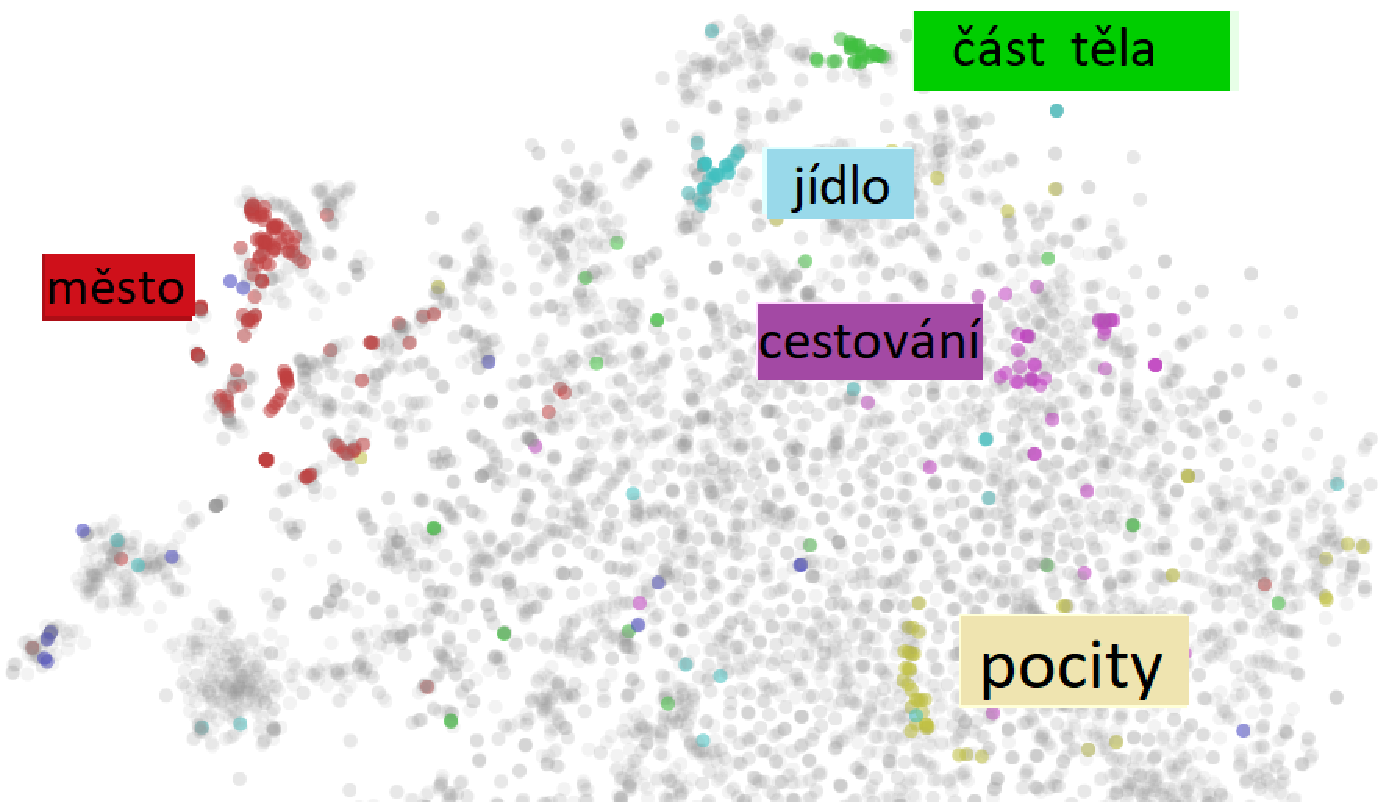
\includegraphics{obrazky/word_represent.pdf}}
	\caption{Část vektorového prostoru znázorňující reprezentace slov, které spojuje nějaké téma. (\url{https://ruder.io/word-embeddings-1/}))}
	\label{word_embeddings}
\end{figure}
%=========================================================================

\subsection{Word2vec}

Word2vec je technika prezentována v~článku \cite{mikolov2013embeddings} schopná naučit se vektorové reprezentace pomocí prediktivního modelu neuronové sítě. Základním konceptem dvou přístupů, které se pro trénink modelu používají, je predikce slov na základě sousedních slov v~tzv. kontextovém okně, které se postupně posouvá. Dostáváme tedy pro každé slovo pravděpodobnost, se kterou se bude vyskytovat v~blízkosti slova cílového.\par
První model používaný pro trénink word2vec vektorů se nazývá Continuous Bag of Words, neboli CBOW. Neuronová síť se trénuje hádáním chybějícího slova v~kontextu známých sousedním slov kontextového okna.\par
Druhá metoda funguje funguje na opačném principu a~nazývá se Continuous Skip-gram Model. Na základě současného slova se tedy model snaží předpovědět slova v~určitém vzdálenosti před, i po současném slově, v~závislosti na velikosti kontextového okna. Tato metoda se z~článku \cite{mikolov2013embeddings} jeví jako o~něco úspěšnější a~je dále zdokonalena v~článku \cite{mikolov2013_2}.\par
Na obrázku \ref{cbow_and_skipgram} můžeme vidět rozdíl v~tom, jak projekční vrstva transformuje vstup na výstup v~případě obou architektur.

\begin{figure}[hbt]
	\centering
	\scalebox{0.5}{
	    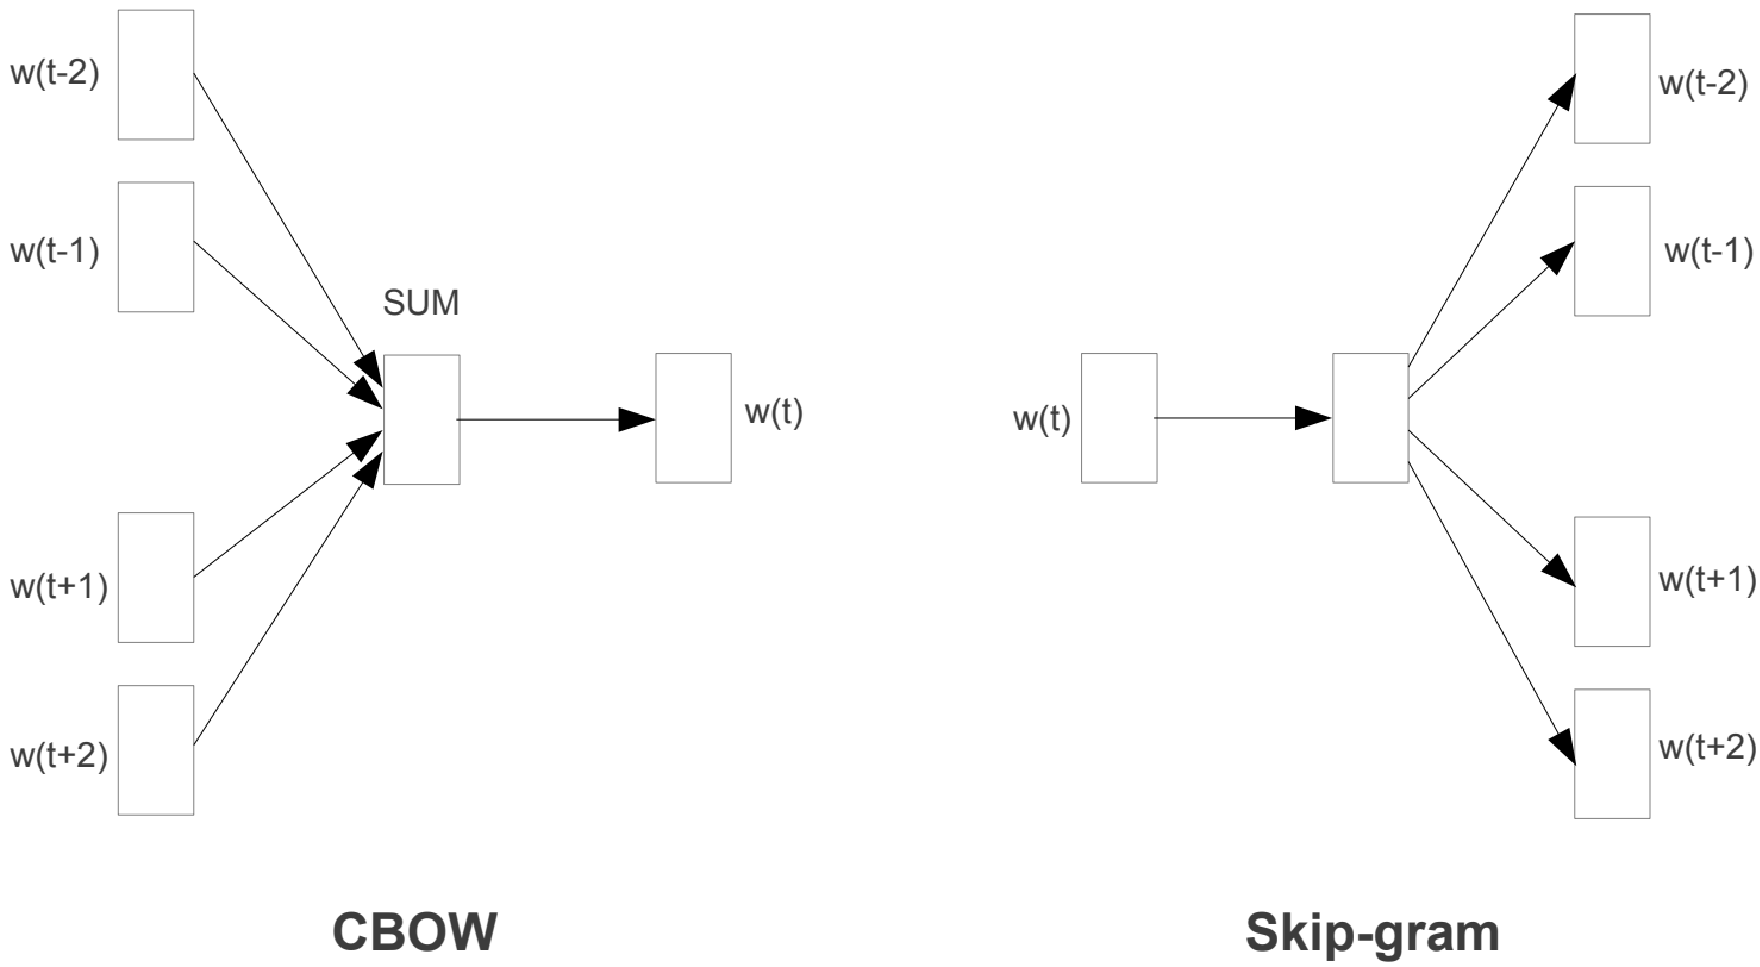
\includegraphics{obrazky/cbow_skipgram.pdf}}
	\caption{Obrázek architrektury CBOW přepovídající slovo na základě kontextu a Skip-grap předpovídající kontext na základě slova. Převzato z \cite{mikolov2013embeddings}.}
	\label{cbow_and_skipgram}
\end{figure}

%=========================================================================

\subsection{GloVe}

GloVe, neboli Global Vectors for Word Representation je technika prezentována v~článku \cite{GloVe}. Výsledkem je vektorový prostor o~pevně dané dimenzi stejně, jako u~word2vec reprezentace. Liší se však způsobem získání daných reprezentací.\par Zatímco word2vec je prediktivní model, GloVe je spíše modelem statistickým. Klade tedy důraz hlavně na počet výskytů slov a~počet jejich výskytů v~podobných kontextech. Dostaneme tedy nějakou matici společných výskytů slov v~korpusu.\par
Jeho hlavní výhodou je, že se nesoustředí pouze na slova v~těsném kontextu, jak už slovo \emph{Global}, ukryté v~GloVe, napovídá. Reprezentace je tedy schopná zachytit sémentické souvislosti v~širším kontextu, ale základní idea není konceptu word2vec příliš daleko.

%=========================================================================

\subsection{Wordpiece embeddings}
\label{wordpiece_embb}
Wordpiece je prediktivní technika prezentována článkem \cite{wordpiece} v~roce 2016 (původně představeno pro strojový překlad) a~používána modely popsanými v~sekci \ref{bert_albert}.\par
Hlavním záměrem přístupu je lépe se vypořádat s~ojedinělými slovy tak, že jsou slova rozdělena do již známých \emph{podslov}. Nabízí tím kompromis mezi \emph{word embeddings} pro celá slova a~tzv. \emph{character embeddings} pro jednotlivé znaky.\par
Slovník je nejprve naplněn všemi znaky v~textu a~jazykový model je na tomto slovníku trénován. Z~výsledného slovníku modelu je poté sestaven slovník nových kombinací jednotlivých znaků tak, aby se zlepšila úspěšnost na trénovací datové sadě. Postup se opakuje, dokud nenarazíme na limit minimální velikosti slovníku, nebo je rozdíl mezi úspěšností jednotlivých iterací modelu příliš malý.

%=========================================================================
\section{Tokenizace a~předzpracování}
\label{preprocessing}
Zpracování textu je důležitou součástí oblasti zpracování přirozeného jazyka. S~textem se totiž pracuje lépe, pokud jsme schopni odstranit některé záludnosti a~nadbytečnosti přirozeného jazyka a~dostat ho do podoby, který je pro automatické zpracování vhodnější. Jednotlivé nástroje pro efektivní zpracování textu v~práci jsou poté uvedeny v~části \ref{pouzite_nastroje}.\par
První část této sekce navazuje na část \ref{reprezentace_slov} o~reprezentaci jednotlivých slov textu a~zabývá se postupem rozdělení textu na tzv. \emph{tokeny}, které mohou být později převedeny na jejich vektorovou reprezentaci.\par
Druhá část je věnována postupům pro zpracování a~pokud možno normalizaci textu pro optimální využití vyhledávacích algoritmů. Statistické metody využívány těmito algoritmy jsou efektivnější, pokud jsou z~textu odstraněny například slova nesoucí zanedbatelnou informaci. Mohou být také zmateny různými tvary daných slov.

\subsection{Tokenizace vstupního textu}
\textbf{Tokenizace} je převod textu jako posloupnosti jednotlivých znaků na posloupnost jednotlivých tokenů. Například rozdělení textu \uv{Adam šel po škole domů.} na posloupnost jednotlivých tokenů:
\begin{center}
    \_Adam $+$ \_šel $+$ \_po $+$ \_škole $+$ \_domů $+$ \_.
\end{center}
Primitivní přístup je rozdělení textu pomocí bílých znaků a~interpunkčních znamének, který ale nebere ohled např na tečky uprostřed zkratek v~angličtině a~těžko se vypořádává se složeninami. Získané tokeny je pak taky třeba normalizovat pro následný převod na word embeddings.\par
V~přístupu uvedeném v~sekci \ref{wordpiece_embb} jsou slova děleny na tokekeny podle toho, která podslova v~daném textu jsou slovníku známy. Můžeme si uvést příklad z~angličtiny, s~jímž podobným se ještě jistě setkáme i v~sekci \ref{bert_albert}. Věta \uv{I~like playing.} by tedy byla převedena na následující tokeny:
\begin{center}
    \_I $+$ \_like $+$ \_play $+$ \_ing $+$ \_.
\end{center}
Na uvedeném případě je vidět hlavně převedení posloupnosti znaků \uv{playing} na dvě podslova (tokeny) \emph{play} a~\emph{ing}.

\subsection{Normalizace délky textu a~rozdělení do vět}
V~kontextu práce je normalizací délky textu myšlena jakási standardní maximální délka dokumentu, který je později předložen readeru k~vyznačení správné odpovědi. Tento přístup je užitečný ze několika důvodů.\par
Algoritmy pro řazení dokumentů dle relevance sice berou na relativní délku každého textu ohled, nicméně některé články jako \cite{bm25_too_long} nasvědčují, že můžou být příliš dlouhé dokumenty znevýhodněny. Článek \cite{bm25_too_long} sice představuje úpravu klasického algoritmu pro minimalizaci tohoto problému, v~práci jsou ale i další důvody, proč je vhodné délku jednotlivých odstavců normalizovat.\par
Model pro vyznačení správné odpovědi v~textu je trénován na datové sadě, která příliš dlouhé dokumenty nebere v~úvahu\footnote{Pro každou otázku je jen jeden odstavec kontextu, ne celý článek z~Wikipedie.} a~jak je naznačeno v~článku \cite{QA_long_multiple_span}, není na dlouhých dokumentech příliš úspěšný.\par
Dalším důvodem je snaha nepřekládat pro účel vyznačení správné odpovědi příliš dlouhé úseky textu.\footnote{Hlavně kvůli určitým omezením dostupných nástrojů pro překlad.}

\paragraph{Proč rozdělit text do vět?}
Předpokládejme, že je text již rozdělen do jednotlivých odstavců. Pro každý odstavec je kontrolována jeho délka, jestli nepřesahuje délku maximální. Pokud bude maximální délka odstavce překročena, může být sice rozdělen jednoduše na poloviny, na třetiny a~tak dále podle potřeby, bude tím ale ztracena velká část kontextu při rozdělení některých vět v~půlce.\par
Pro takový případ je vhodné vědět, kde jednotlivé věty začínají a~končí, aby bylo možné jednotlivé odstavce případně smysluplně rozdělit. Vhodné je také zařídit, aby se jednotlivé rozdělené \uv{pododstavce} částečně překrývaly a~obsahovaly třeba 3 poslední věty odstavce předchozího, pro maximální zachování původního kontextu.

\subsection{Převod na malá písmena}
\label{prevod_na_mala}
Převod na malá písmena je sice velmi jednoduchý, ale přesto užitečný úkol. Při psaní otázky na klávesnici je velmi pravděpodobně, že pomyslný uživatel napíše \uv{sssr} místo \uv{SSSR} nebo \uv{Albert} místo \uv{ALBERT}, ale bylo by vhodné, aby byly nalezeny dokumenty obsahující obě varianty. Stejně tak může dojít k~nestandardnímu užití malých/velkých písmen v~některém z~dokumentů.\par
Pro některé případy může převod na malá písmeny znamenat ztrátu části kontextu. Například \emph{Malá Strana} X \emph{malá strana}, kde velké písmeno indikuje vlastní jméno (městskou část). Vhodné je to tedy pouze v~některých případech.

\subsection{Odstranění stop slov}
\label{stopwords}
Ve zpracování přirozeného jazyka jsou \emph{stop slova} většinou souborem nejčastěji používaných slov v~daném jazyce\footnote{\url{https://en.wikipedia.org/wiki/Stop_word}}. Většinou jsou odstraňována, protože kvůli jejich vysokému výskytu nesou menší informační hodnotu a~jejich odstranění vede k~lepší funkci vyhledávacích algoritmů \cite{bm25_improvements}.\par
Nejužívanější slova daného jazyka je možno najít například ve frekvenčních seznamech, které obsahují nejpoužívanější slova v~češtině. Získaný seznam je vhodné kriticky zhodnotit a~vyčlenit z~něj některá slova, která by pro vyhledávání mohla mít kritický význam.\footnote{Příklad: \uv{první}, \uv{země}, \uv{člověk} \dots} Většinou je zanedbatelná alespoň většina spojek, předložek či zájmen. Typickými příklady stop slov pro češtinu jsou: být, a, se, v, že \dots

\subsection{Získání lemmat}
\textbf{Lemmatizace} je druh zpracování textu, při kterém je pro každé slovo nalezen základní tvar, tzv. \emph{lemma}.\footnote{Podobným postupem je \emph{stematizace}, která ale algoritmicky pouze odstraní koncovky a~předpony pro nalezení slovního kmene. Lemmatizátor pro nalezení základních tvarů používá morfologický slovník.}
\begin{center}
    ulicí běžely děti $\longrightarrow$ ulice běžet dítě\\
    ostrovy Středozemního moře $\longrightarrow$ ostrov Středozemní moře
\end{center}
Pro získání lemmat se používají speciální nástroje pro zpracování přirozeného jazyka. \emph{Lemma\-tizátory} mohou poskytovat také některé doplňkové informace o~mluvnichkých kategoriích jako rod, pád nebo slovní druh. Hlavním úskalím lemmatizátorů je mnohoznačnost jazyků jako je čeština, kdy může být více základních tvarů daného slova dle kontextu \footnote{\url{https://cs.wikipedia.org/wiki/Lemmatiz\%C3\%A1tor}}.\par
Využití lemmatizace je různé, ale v~případě této práce je podobné, jako účel postupu uvedeného v~sekci \ref{prevod_na_mala}. Jednoduše se hodí, když pro dotaz obsahující \uv{\dots Liparských ostrovů} budou nalezeny i dokumenty obsahující základní tvar hledaného výrazu \uv{Liparské ostrovy}\par
Lemmatizace je také užitečným nástrojem při odstranění stop slov, kdy můžeme například odstranit všechny tvary slovesa \uv{být}, zatímco seznam stop slov může obsahovat pouze jeho základní tvar.


%=========================================================================
%===============================================================================

\chapter{Strojové učení pro extrakci odpovědi}
\label{language_comprehension}

Rozmach strojového učení umožnil obrovský pokrok v~oblastech NLP jako strojový překlad, rozpoznání entit, generování textu nebo také odpovídání na otázky. Proto na tomto přístupu staví všechny nejmodernější metody a~tímto směrem se také ubírá výzkum.\par
Účelem této kapitoly je vysvětlit čtenáři, jak fungují neuronové sítě a~jakým způsobem dokáže počítač porozumět textu a~naučit se vyznačit v~textu odpověď na danou otázku.\par
Nejprve budou ve zkratce vysvětleny principy fungování a~učení neuronových sítí. Poté budou rozebrány nejznámější architektury neuronových sítí používané pro vypořádání se s~úkoly na poli zpracování přirozeného jazyka a~nakonec budou popsány nejmodernější modely, které na nich staví.
\bigskip

%=========================================================================
\section{Neuronové sítě}
\label{neuronove_site}
V~této části bude vysvětlen princip fungování neuronových sítí. Informace v~sekci byly převzaty z~článku \cite{neural_nets} a~z~prezentací Stanfordského kurzu NLP.\footnote{Dostupné z: \url{http://web.stanford.edu/class/cs224n/}}\par
Neuronové sítě si můžeme zjednodušeně představit jako velkou funkci s~obrovským množstvím parametrů, která přetváří vstupy na výstupy. V~průběhu tréninku neuronové sítě se postupně všechny parametry optimalizují tak, aby síť přetvářela vstupy na výstupy co nejlépe.\par
Fungují tu tři základní jednoduché vrstvy(\ref{three_layers}). Vstupní, skrytá (zde probíhá proces přetváření vstupů) a~výstupní, na které se přetvořený vstup objeví. Skrytá vrstva se navíc běžně skládá z~mnoha dalších vrstev.\par
Každá z~těchto vrstev, ať už je vstupní, výstupní, nebo skrytá, se skládá z~dalších primitiv a~ty jsou nazývány jak jinak, než neurony. Každý neuron v~každé vrstvě je propojen s~každým neuronem vrstvy další, a~tak je propojena celá síť.

\begin{figure}[hbt]
	\centering
	\scalebox{0.50}{
	    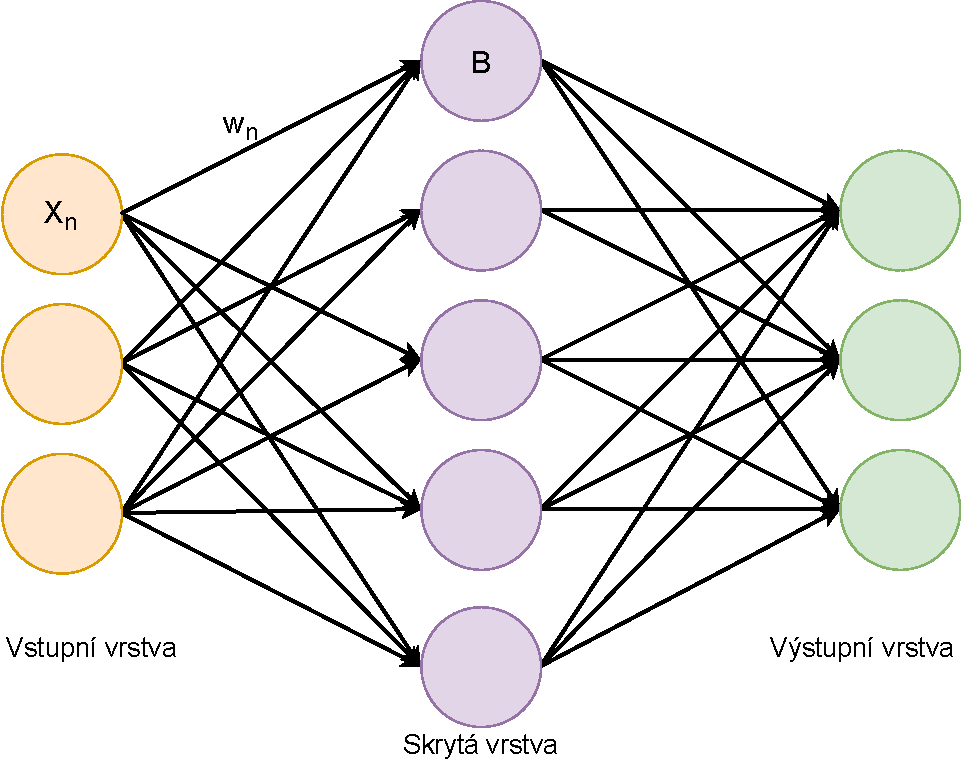
\includegraphics{obrazky/neural_net.pdf}}
	\caption{Schéme neuronové sítě s jednou skrytou vrstvou. Znázorněn je také práh neuronu $B$, jeden vstup z předchozí vrstvy $x_n$ a váha jednoho propojení $w_n$.}
	\label{three_layers}
\end{figure}

\subsection{Umělý neuron a~aktivační funkce}
Umělý neuron je primitivní jednotka inspirována neuronem skutečným. Ten vypadá asi tak, že má tělo, do kterého přichází krátkými výběžky, tzv. \emph{dendrity} elektrické signály z~ostatním neuronů. Z~těla tohoto neuronu pak vychází jediný dlouhý výběžek, tzv. \emph{axon}. Neuron se tedy na základě signálů, které do něj přichází dendrity rozhodne (na základě nějaké minimální hranice přijatého signálu), zda-li bude, nebo nebude vysílat signál dál \footnote{\url{https://cs.wikipedia.org/wiki/Neuron}}.\par
Funkce umělého neuronu je analogická. Jak už bylo popsáno v~úvodu sekce \ref{neuronove_site}, každý neuron je propojen s~každým neuronem vrstvy předcházející i vrstvy další. Na rozdíl od skutečného neuronu má tedy \uv{více axonů}, kterými je propojen s~další vrstvou.\par
Každé propojení mezi každým neuronem má svoji váhu \emph{w}, která ovlivňuje důležitost jednotlivého vstupu do neuronu. Každý neuron má pak svůj práh \emph{B} a~aktivační funkci. Výstupem neuronu je tedy vážená suma vstupů do neuronu s~přičteným prahem a~aplikovanou aktivační funkcí, neboli 
\begin{equation}
F({\sum_{i=1}^n ({x_n}w_n)} + B)
\end{equation}
kde $x_n$ je neuron předcházející vrstvy, $w_n$ je váha jeho propojení, $B$ je práh aktuálního neuronu a~$F$ je aktivační funkce. Znázornění vah propojení a~jednotlivých neuronů je vyznačeno na obrázku \ref{three_layers}.\par
Všechny propojení jednotlivých neuronů a~jejich prahy v~dávají dohromady parametry neuronové sítě, které jsou v~průběhu tréninku optimalizovány pro každý neuron zvlášť. Pro síť, jako je na obrázku \ref{three_layers} je to třeba 30 jednotlivých vah propojení a~8 prahů jednotlivých neuronů (skryté a~výstupní vrstvy), tedy 38 parametrů v~tak jednoduché síti.\par
\textbf{Aktivační (přenosová) funkce} rozhoduje, jestli bude daný neuron aktivován. Skutečný neuron má, zdá se, funkci skokovou. Umělé neurony však používají funkce s~postupnou aktivací. Běžné jsou tři (čtyři) základní varianty aktivačních funkcí: 

\begin{itemize}
    \item (Skoková)
    \item Sigmoidální
    \item Hyporbolické tangenty
    \item ReLU (Rectified Linear Unit)
\end{itemize}

Funkce jsou znázorněny na obrázku \ref{aktivacni_funkce}. Vhodnost použití každé z~nich může být různé. Výhodou sigmoidální funkce je normalizace výstupu do rozmezí $(0,1)$. Nejpoužívanější funkcí pro skrytou vrstvou je však funkce ReLU. Kvůli její charakteristice je aktivováno méně neuronů, což vede k~rychlejšímu tréninku a~konvergenci. Použití ReLU funkce je také méně výpočetně náročné \cite{medium:activation_function}.

\begin{figure}[hbt]
    \centering
	    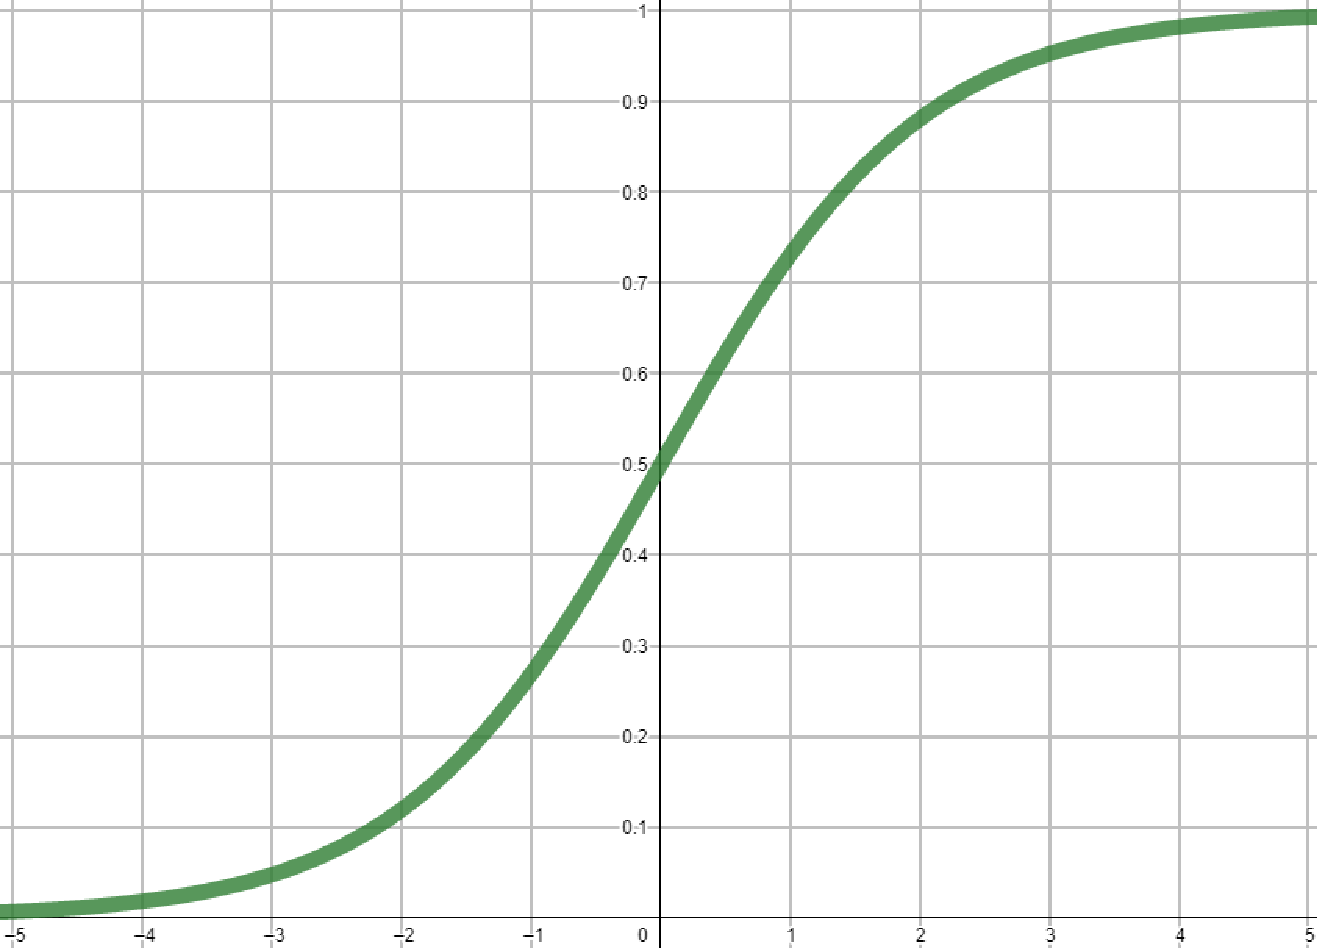
\includegraphics[width=0.33\linewidth, height=1.5in]{obrazky/sigmoid.pdf}\hfill
    	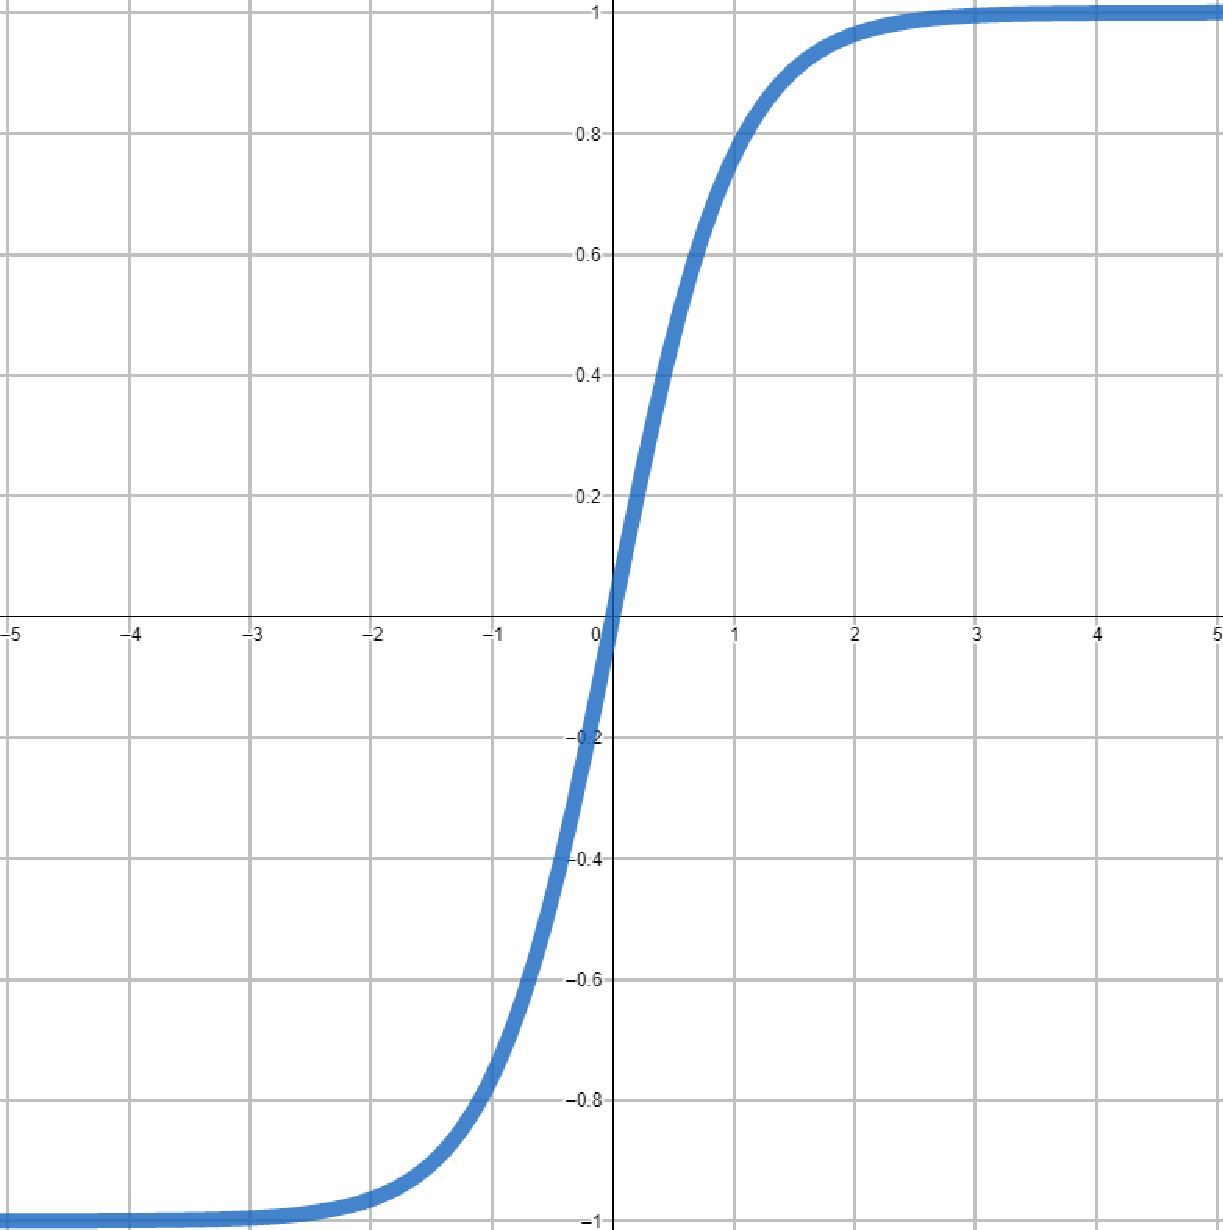
\includegraphics[width=0.33\linewidth, height=1.5in]{obrazky/tanh.pdf}\hfill
    	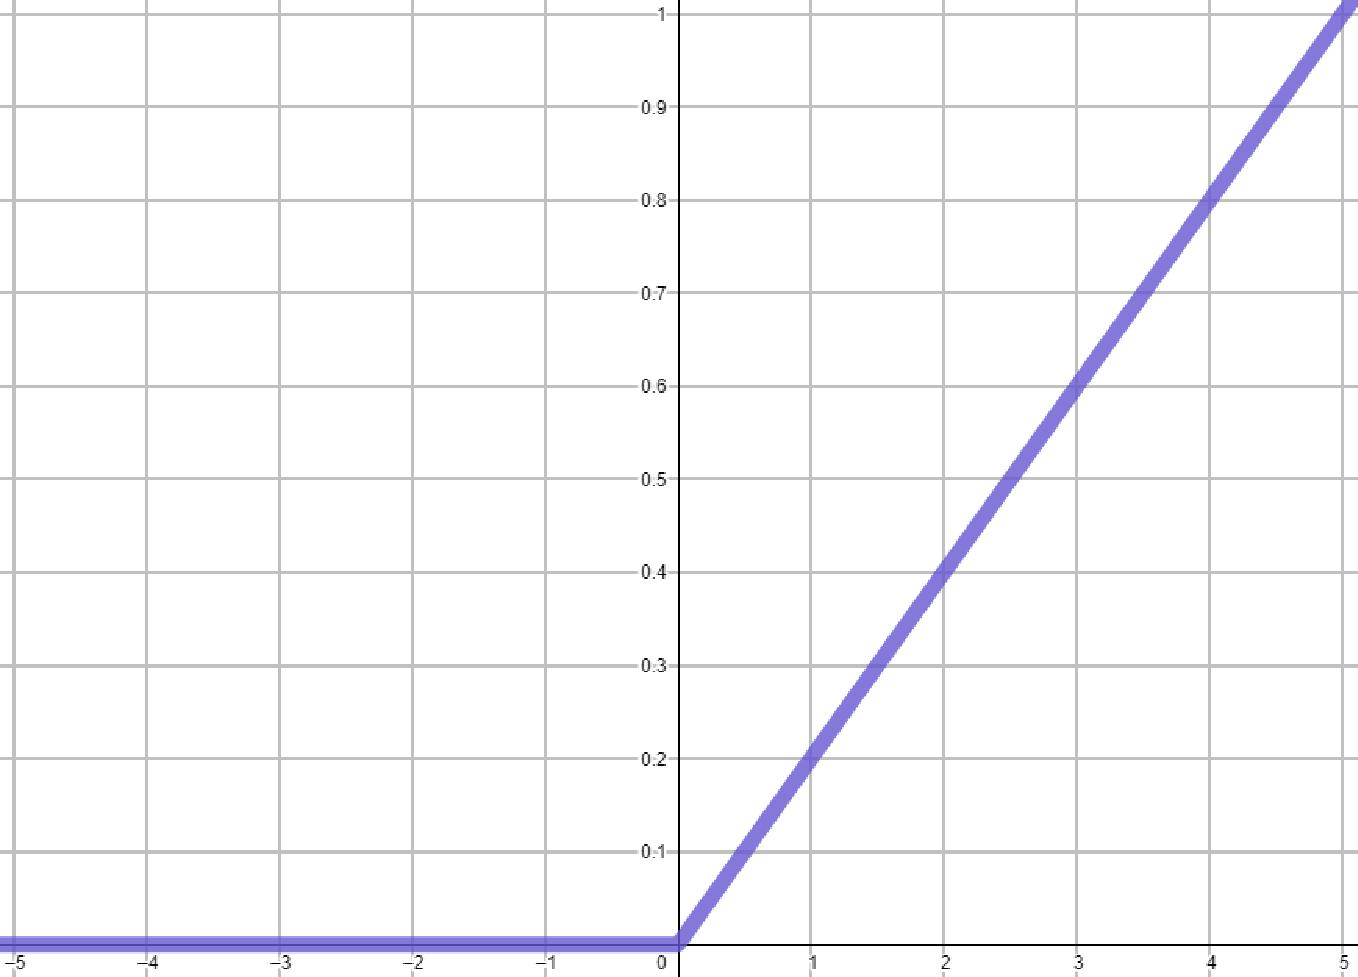
\includegraphics[width=0.33\linewidth, height=1.5in]{obrazky/relu.pdf}\hfill
	\caption{Jednotlivé aktivační funkce, zleva: sigmoidální ($H(f)=\langle 0,1 \rangle$), hyperbolické tangenty (tanh $H(f)=\langle -1,1 \rangle$) a ReLU ($H(f)=\langle 0,\inf \rangle$).}
	\label{aktivacni_funkce}
\end{figure}


\subsection{Dopředná a~zpětná propagace}
Proces, kdy se opakovaně ze vstupů počítá výstup každého neuronu v~dané vrstvě a~stejně tak pro každou následující vrstvu, se nazývá dopředná propagace. Tímto postupem se postupně hodnoty vstupní vrstvy přetvoří na hodnoty ve vrstvě výstupní a~může se určit, jak byla síť úspěšná.\par
Pro určení úspěšnosti každé takové iterace neuronové sítě se používá nákladová funkce (anglicky cost function pro jednu iteraci, loss function pro průměr všech), která udává jediné číslo charakterizující úspěšnost modelu. Nejznámější nákladovou funkcí je Střední kvadratická chyba (anglicky Mean Squared Error - MSE). Cílem je hodnotu této nákladové funkce postupně minimalizovat.\par \medskip
Postup optimalizace jednotlivých parametrů neuronové sítě pro zajištění minimalizace nákladové funkce se nazývá \textbf{zpětná propagace}. Je to v~podstatě opačný průchod neuronovou sítí, který má za úkol zjistit, které neurony se největší mírou podílely na výsledné chybě. Snížením významu těchto neuronů můžeme dosáhnout lepší úspěšnosti celé sítě. Naopak můžeme zvýšit význam propojení s~neurony, které výstup ovlivnily pozitivně.\par
Základem tohoto výpočtu je, že chyba každého výstupního neuronu je vstupem parciální derivace vzhledem ke každému z~jeho vstupů. Celý postup zpětné propagace je velmi složitý a~pro intuitivní pochopení problematiky není klíčový, proto tu nebude podrobně rozebrán.\par
Celý postup zpětné propagace je opakován a~parametry neuronové sítě jsou postupně optimalizovány.\par \medskip
Trénink neuronové sítě tedy probíhá následovně. Síti s~náhodně inicializovanými parametry je předložena část dat z~trénovací datové sady. Ty jsou pomocí dopředné propagace prostupem přes skrytou vrstvu přetvořeny na výstupy a~tím získány predikce neuronové sítě. Predikce jsou porovnány se základní pravdou (tzv. \emph{ground truth}) a~nákladovou funkcí je vyjádřeno, jak byly predikce daleko od pravdy. Pomocí zpětné propagace jsou postupně upraveny všechny parametry neuronové sítě.\par
Postup je opakován, dokud úbytek nákladové funkce mezi jednotlivými iteracemi nezačne dlouhodobě stagnovat, nebo dokud nedosáhneme požadovaného počtu epoch.\par
Při nesprávném tréninku neuronové sítě může dojít k~podtrénování (underfitting), nebo přetrénování (overfitting). Problémy při tréninku souvisí s~tzv. hyperparametry, mezi které patří počet skrytých vrstev, velikost modelu nebo \emph{learning rate}\footnote{Konstanta určující velikost kroku při každé iteraci zpětné propagace při úpravě parametrů neuronové sítě.}. Pomoct může také množství trénovacích dat nebo počet trénovacích epoch.

%=========================================================================
\section{Nejlepší architektury pro porozumění textu}
V~této sekci budou popsány dvě nejznámější a~nejpoužívanější architektury používané pro zpracování přirozeného jazyka. Rozšiřují koncepty prezentované v~sekci \ref{neuronove_site} a~snaží se překonat problémy, které tradiční model představuje.\par
První model v~části \ref{lstm} využívá k~překonání ztráty kontextu rekurentní neuronové sítě. Druhý model v~části \ref{transformers} spoléhá na paralelní zpracování a~vzájemnou pozornost mezi otázkou a~kontextem.

\subsection{Long short-term memory}
\label{lstm}
Informace v~této sekci byly převzaty z~originální práce \cite{LSTM}, která architekturu představuje a~ze článku \cite{understandingLSTM}.\par
LSTM, neboli Long Short-term Memory je speciální druh \emph{rekurentní} neuronové sítě, který se částečně vypořádává s~problémem ztráty kontextu v~delším úseku textu. Jednoduše řečeno, při učení neuronové sítě bychom byli rádi, aby pochopení současné věty dokázala ovlivnit i věta předcházející.\par

\begin{figure}[hbt]
    \centering
	\scalebox{0.9}{
	    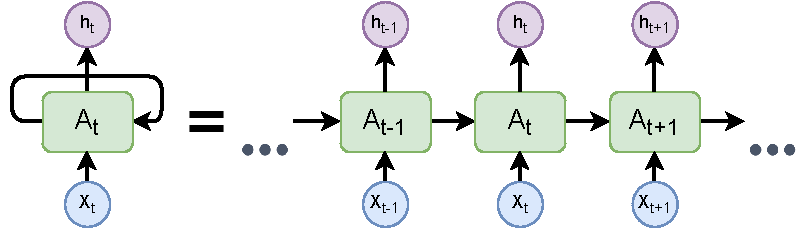
\includegraphics{obrazky/rnn.pdf}
	}
	\caption{Schéma rekurentní neuronové sítě inspirován obrázkem z \cite{understandingLSTM}. $X_t$ je vstupem neuronové sítě $A_t$ v čase $t$ a výstupem $h_t$.}
	\label{RNN}
\end{figure}

Nejprve bude vysvětlen princip \textbf{rekurentní neuronové sítě} (dále RNN - Recurrent Neural Network).
Jejich hlavním úkolem je vypořádat se se zpracováním sekvenčních dat, jako je text. Oproti například rozpoznávání vzorů v~obrázcích není možné pohlížet na každé slovo v~textu zvlášť. Slovo/slova předcházející by měly ovlivnit slovo současné. Stejně tak by měly následující slova ovlivnit význam slova současného (obousměrné rekurentní sítě).\par
Schéma jednoduché RNN je vidět na obrázku \ref{RNN}. Zjednodušeně je to tedy více jednoduchých neuronových sítí propojených za sebe. Vstupem každé sítě $h_n$ je výstup předchozí sítě $h_{n-1}$ a~slovo $x_n$. Výstup $y_n$ je potom vstupem do další jednotky $h_{n+1}$.\par
Analogicky funguje obousměrná RNN, které je propojená i v~opačném směru. Vstup je zpracováván od konce a~pro současné slovo je tedy brán v~úvahu i kontext slova nadcházejícího, jak je vidět na obrázku \ref{bidirRNN}.\par

\begin{figure}[hbt]
    \centering
	\scalebox{0.9}{
	    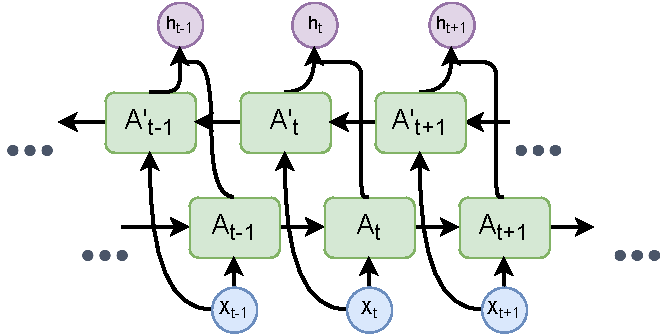
\includegraphics{obrazky/bidir_rnn.pdf}
	}
	\caption{Schéma obousměrné rekurentní neuronové sítě.}
	\label{bidirRNN}
\end{figure}

\pagebreak\textbf{LSTM} (Long Short-term Memory) představuje vylepšení standardní RNN.\par \smallskip
Mějme model, který má za úkol předpovědět následující slovo ve větě. Pokud se kontext potřebný pro predikci nachází v~těsné blízkosti předpovídaného slova (př.: \uv{vychlazené mléko z~\emph{lednice}}), je i běžná RNN schopná si souvislost propojit. Pro příklad, kdy je kontext \uv{dále v~minulosti} (př.:\uv{Učím se od 6 let anglicky \dots Vzhledem k~těmto okolnostem plynule ovládám \emph{angličtinu}}) není RNN schopná naučit se tuhle souvislost mezi kontextem a~hledaným slovem.\par \smallskip
LSTM je tedy narozdíl od klasické RNN navržená tak, aby byla schopná pamatovat si dlouhodobé souvislosti v~textu při sekvenčním zpracování. Řeší tím tzv. \emph{problém mizejícího gradientu}.\par
Model má stejnou opakující se strukturu jako RNN, rozdíl je však v~komplexnosti opakující se jednotky (či buňky). Struktura naznačená na obrázku \ref{lstm_cell} je poměrně složitá a~jejím hlavním komponentem jsou tzv. \emph{brány}. 

\begin{figure}[hbt]
    \centering
	\scalebox{1}{
	    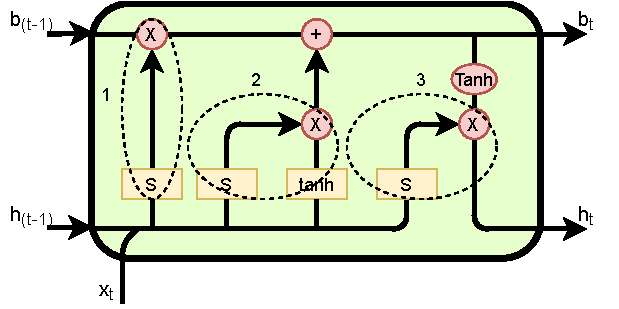
\includegraphics{obrazky/lstm_cell.pdf}
	}
	\caption{Schéma LSTM buňky převzato z článku \cite{understandingLSTM}. $b_t$ je vnitřní stav buňky, $b_{(t-1)}$ předcházející buňky, $h_t$ výstup buňky, $h_{(t-1)}$ výstup předcházející. $x_t$ je vstup současné buňky. \uv{1} je \emph{zapomínací}, \uv{2} \emph{vstupní} a \uv{3} \emph{výstupní} brána.}
	\label{lstm_cell}
\end{figure}

Brány jsou v~LSTM buňce celkem tři. Každá je složena z~vrstvy neuronové sítě se sigmoidální funkcí (\uv{S} v \ref{lstm_cell}) a~násobícího (\uv{$\times$} v \ref{lstm_cell}) operátoru. Brána je komponentem určujícím, kolik informace je možno propustit. Brány budou popsány zleva doprava.\par
První, tzv. zapomínací brána určuje, kolik vstupní informace je zahozeno\footnote{Výstupem je číslo v~rozmezí (0,1), kde 0 znamená \uv{všechno zahodit} a~1 znamená \uv{všechno propustit}.}. Druhá, tzv. vstupní brána, určí, které hodnoty skrytého stavu buňky budou aktualizovány a~vrstva s~funkcí \emph{tanh} (\uv{tanh} v \ref{lstm_cell}) rozhodne o~nových kandidátních hodnotách, které po kombinaci s~výstupem sigmoidální vrstvy vytvoří nový skrytý stav buňky. Poslední bránou je výstupní, která spojuje informaci z~brány zapomínací a~vnitřním stavem buňky a~vytváří tím tedy výstup dané buňky.\par
Jednotlivé LSTM buňky jsou za sebou sekvenčně propojeny stejně jako RNN. Při použití dvou LSTM sítí s~tou druhou propojenou v~opačném směru získáme obousměrnou LSTM síť. Výstupy obou sítí jsou poté pro získání výstupu zřetězeny.

\subsection{Transformers}
\label{transformers}
Informace v~této sekci byly převzaty z~originální práce \emph{Attention Is All You Need} \cite{Transformers}, práce \cite{attention_mechanism} a~článku \cite{Transformers-explained}. Sekce popisuje Transformer model používaný pro zpracování přirozeného jazyka a~mechanismus pozornosti, který s~ním úzce souvisí.\par
Přístup použitý tímto modelem se dokázal oprostit od rekurentních modelů jako LSTM a~nahradil je na poli zpracování přirozeného jazyka jako nová state of the art architektura. Transformers nepoužívá sekvenční zpracování slov, ale zpracování paralelní.\par
Jeho nejdůležitější myšlenkou je tzv. \textbf{mechanismus pozornosti} (anglicky \emph{attention mechanism}) představený článkem \cite{attention_mechanism} původně pro strojový překlad. Mechanismus pozornosti se však dále rozvíjel a~popularizoval do dalších odvětví strojového učení. Stručně bude tedy popsán.\par \medskip

Mechanismus vezme vektory dvou vět přirozeného jazyka naráz a~sestaví z~nich \emph{key(\textbf{K})-value(\textbf{V})} a~\emph{query(\textbf{Q})} matice (řádek -- vektor pro každé vstupní slovo). Ty vzniknou vynásobením vstupní word embedding matice speciální váhovou maticí, jejíž parametry se natrénují. Na matice jsou poté aplikovány následující operace pro získání výstupu attention mechanismu

\begin{equation}
    \label{attention_dot_product}
    softmax(\frac{Q \times K}{k})\times V
\end{equation}

kde k~je podle \cite{Transformers} konstanta 8 (mohly by bý stanoveny i jiné hodnoty) a~softmax funkce pro normalizaci výstupu do rozmezí (0,1).\par
Vektory pro všechny vstupní slova respektive vstupní matice K, V~a Q mohou být ze stejné věty. Potom se používá termín \textbf{self-attention}.\par
Tím je určeno, která část vstupu je relevantní (self-attention), nebo například která část dokumentu je relevantním kontextem dané otázky.\par
Jednoznačnou výhodou mechanismu pozornosti je, že je schopen podívat se na celý kontext naráz (narozdíl od RNN, která prochází vstup sekvenčně) a~vyznačit v~něm důležité pasáže. Tímto se zbavuje problému mizejícího gradientu.\par\medskip

\textbf{Transformer} enkodér\footnote{Enkodér je část modelu, která vytvoří z~vektorů jednotlivých slov na vstupu vektor celého vstupního textu, reprezentující jeho význam.}\footnote{V původním článku představen model pro \emph{sequence to sequence} model vhodný pro překlad, který obsahuje i dekodér pro generování textu.} je model, jehož architektura je kombinací dopředné neuronové sítě a~mechanismu pozornosti. Jak už bylo popsáno, jeho hlavní výhodou je vlastnost\linebreak \emph{mechanismu pozornosti} zpracovávat vstupní slova paralelně, a~tím se naučit i vztahy mezi slovy na dlouhé vzdálenosti v~textu.\par

\begin{figure}[hbt]
    \centering
	\scalebox{1}{
	    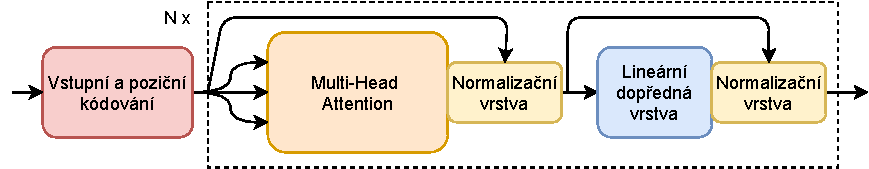
\includegraphics{obrazky/transformer_encoder.pdf}
	}
	\caption{Schéma architektury transformer enkodéru převzaté z článku \cite{Transformers}. V článku je uvedeno $N=6$ pro počet identických vrstev ekodéru. }
	\label{transformer_encoder}
\end{figure}

Na obrázku \ref{transformer_encoder} můžeme vidět zjednodušenou strukturu jednotky enkodéru. V~článku \cite{Transformers} tvoří enkodér 6 takových bloků propojených za sebe.\par
Před vstupem do prvního bloku jsou jednotlivé tokeny vstupního textu převedeny na vektory (word embeddings), ke kterým je přidáno poziční kódování\footnote{identifikuje pořadí tokenu ve vstupním textu.}.\par
Každý blok se pak skládá z~\uv{\emph{multi-head attention}} modulu a~plně propojené dopředné vrstvy. Obě části jsou následovány normalizační vrstvou.\par
Nejzajímavější částí bloku enkodéru je multi-head attention modul, který je dále rozkreslen na obrázku \ref{multihead}. Modul je sofistikovanou implementací self-attention mechanismu popsaném dříve, který dokáže vyzdvihnout souvislost jednotlivých částí celého kontextu. 

\begin{figure}[hbt]
    \centering
	\scalebox{0.35}{
	    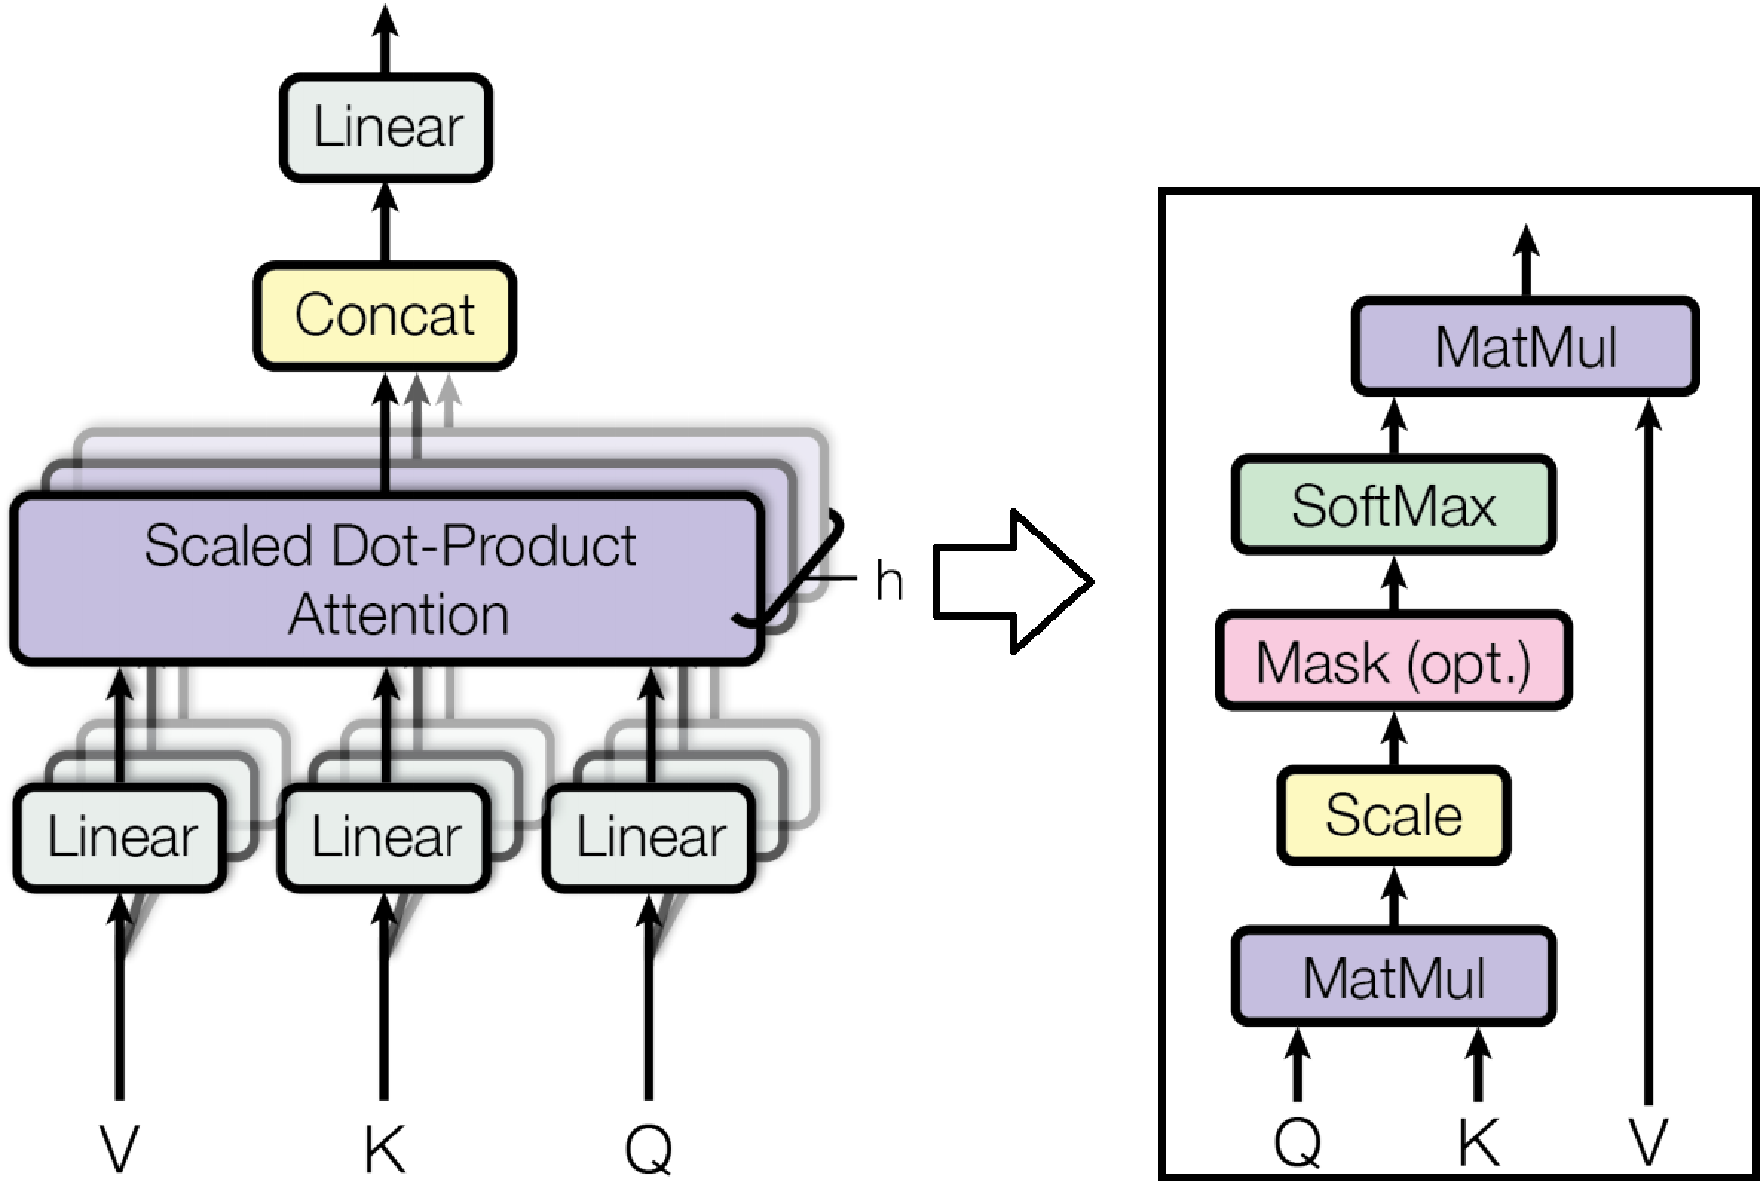
\includegraphics{obrazky/multihead_att.pdf}
	}
	\caption{Schéma \emph{Multi-Head} attention vlevo a \emph{Scaled Dot-Product} attention vpravo. \emph{Multi-head} attention je aplikováno paralelně v $h$ vrstvách (pro práci \cite{Transformers} $h=8$). Obrázky byly převzaty z článku \cite{Transformers}.}
	\label{multihead}
\end{figure}

Mechanismus ne obrázku \ref{multihead} vpravo je popsaný rovnicí (\ref{attention_dot_product}) a~je hlavním komponentem multi-head attention modulu znázorněném v~\ref{multihead} vlevo.\par
Multi-head znamená, že do modulu vstupuje 8 (dle práce \cite{Transformers}) trojic V,K,Q. Každá matice trojice V,K,Q je transformována lieární vrstvou a~na celou trojici je potom aplikován \emph{scaled dot-product attention} (self-attention) mechanismus. Tento postup je aplikován na každou z~osmi trojic paralelně, pokaždé však s~jinými váhami lineární vrstvy.

%=========================================================================
\section{Předtrénované modely BERT a~ALBERT}
\label{bert_albert}

V~této sekci budou představeny modely založené na architektuře Transformer popsané v~sekci \ref{transformers}. Informace v~této sekci jsou převzaty z~původních článků \cite{BERT} a~\cite{ALBERT}.\par
Předtrénované modely stavějící na této architektuře určily nový standard pro přicházející state of the art metody. Kromě jejich vysoké úspěšnosti je obrovskou výhodou také znovupoužitelnost předtřénovaných modelů. Modely je možno jednoduše dotrénovat (provést tzv. \emph{fine-tuning} po načtení modelu s~předtrénovanými parametry) pro celou řadu úkolů na poli NLP, jako je odpovídání na otázky, rozpoznání entit, klasifikace textu a~další.

\subsection{BERT}
BERT (Bidirectional Encoder Representation from Transformers) je model pro reprezentaci přirozeného jazyka představený v~roce 2018 prací \cite{BERT}. Jeho hlavním přínosem je aplikace obousměrného tréninku Transformer architektury. Ukazuje, že model trénovaný v~obou směrech dokáže plně využít schopnost Transformerů zpracovávat vstupní text naráz, ne sekvenčně.\par\smallskip
Hlavním přínosem práce \cite{BERT} je způsob, kterým probíhá předtrénink na velkých textových korpusech. Trénink na úkolech, které nemusí přímo souviset s~cílovým použitím dovolí modelu získat základní pochopení vlastností jazyka pro jeho správnou reprezentaci vytvořenou enkodérem. Pro předtrénink modelu BERT byly použity následující úkoly.

\begin{figure}[hbt]
	\centering
	\scalebox{1}{
	    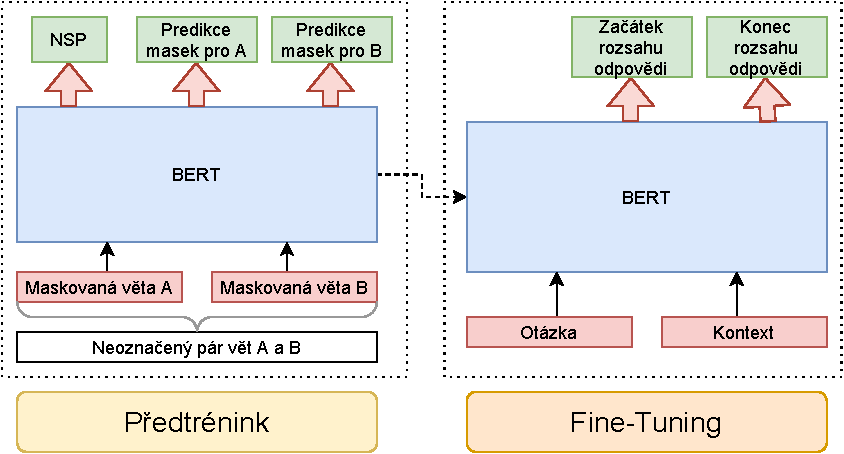
\includegraphics{obrazky/bert_pretraining_fine_tuning.pdf}
	}
	\caption{Vlevo předtrénink ekodéru BERT na úlohách \emph{ML modeling} a \emph{NSP}. Vpravo předtrénovaný BERT dotrénován na konkrétní úlohu odpovídání na otázky. Obrázek byl inspirován obrázkem 1 z článku \cite{BERT}.}
	\label{bert}
\end{figure}

\medskip
\textbf{Maskované modelování jazyka} (ML modeling) 
je úloha velmi podobná již dříve zmíněné úloze predikce následujícího slova ve větě.Je ale použit přístup, kdy je určité procento slov v~textu \emph{maskováno}, aby nebyl původní úkol kvůli obousměrné reprezentaci transformerů triviální.\par
Při tréninku je 15\,\% slov každé věty nahrazeno [MASK] tokenem, jehož původní význam je poté na základě okolního kontextu hádán.\par
Pro tento úkol je na enkodér BERTa napojena klasifikační vrstva, pomocí které je určena pravděpodobnost pro každého slovo ve slovníku, které má [MASK] token nahradit.\par
\smallskip
\textbf{Predikce následující věty} (NSP) je druhým typem úlohy pro předtrénink BERTa. Jeho snahou je naučit model porozumět vztahu nejen mezi jednotlivými slovy, ale taky mezi významem celých vět.\par
Trénovací datová sada je rozdělena na dvojice vět A~a B. Model má za úkol předpovědět, je-li věta B větou následující větu A~v~kontextu. V~50\,\% případů je věta B opravdu větou následující. Ve zbytku je to náhodně zvolená věta z~korpusu.\par
Práce \cite{BERT} také uvádí, že navzdory jednoduchosti tohoto úkolu je jeho přínos pro pozdější aplikaci modelu pro odpovídání na otázky velký.\par

\paragraph{Formát vstupu}
modelu BERT je koncipován tak, aby mohl být použit pro větší spektrum aplikací, pro které je zamýšlen. Proto je umožněno na vstupu pomocí jediné sekvence tokenů reprezentovat jak jednu, tak i dvě vstupní sekvence, jako třeba otázku a~odpověď.

\begin{figure}[hbt]
	\centering
	\scalebox{0.45}{
	    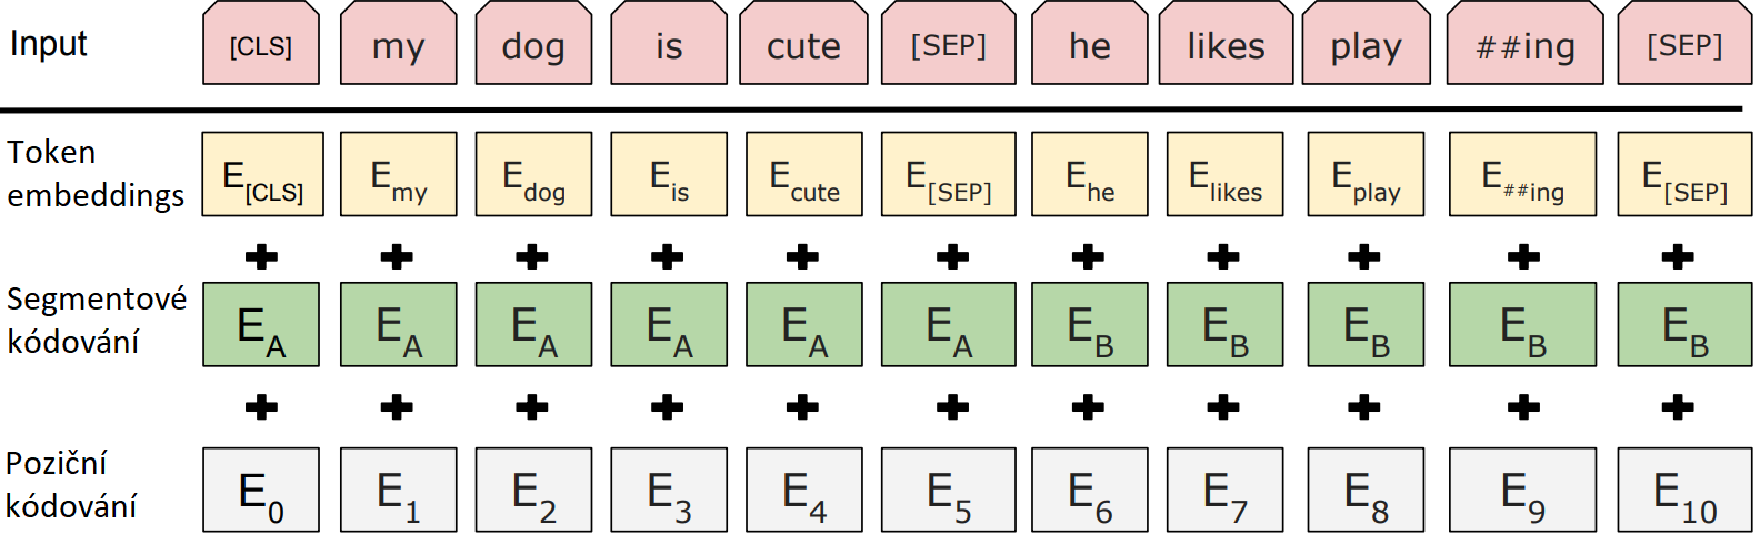
\includegraphics{obrazky/bert_input_new.pdf}
	}
	\caption{Příklad formátu vstupu \uv{\emph{input}} modelu BERT převzatý z \cite{BERT}. Poziční (\emph{position}), segmentové a~token \emph{embeddings} a~speciální tokeny [CLS] a~[SEP].}
	\label{bert_input}
\end{figure}

Pro vektorovou reprezentaci jednotlivých tokenů jsou použity Wordpiece embeddings \cite{wordpiece} popsány v~\ref{wordpiece_embb}. K~těm je přidáno poziční kódování kvůli použití Transformer architektury a~segmentační kódování, které identifikuje, které sekvenci vstupu jednotlivé tokeny náleží. Příklad je naznačen na obr. \ref{bert_input}.\par
Pro popis vstupu jsou navíc použity dva speciální tokeny [CLS] a~[SEP]. [CLS] token je přidán vždy na začátek vstupu. Token [SEP] je přidán na konec každé sekvence. [CLS] token je využit také pro klasifikační úlohy (například předtrénink na NSP).

\subsection{ALBERT}
Informace v~této sekci jsou převzaty ze článku \cite{ALBERT} \emph{A~Lite BERT for self-supervised learning of language representations}.\par
Hlavním problémem modelu jako BERT je jeho velikost -- asi 110 milionů parametrů v~jeho základní verzi. Zvětšováním modelu se většinou dá dosáhnout zlepšení, je to však problém kvůli omezené paměti grafických karet a~množství času potřebného pro trénink.\par
\textbf{ALBERT} -- A~Lite BERT, je model představený v~roce 2019 článkem \cite{ALBERT}. Vychází z~modelu BERT a~dosahuje lepších výsledků na datových sadách pro porozumění textu, přestože má mnohem menší počet parametrů, než velká verze BERTa. V~následujících odstavcích jsou shrnuty hlavní přínosy modelu ALBERT.

\paragraph{Faktorizace parametrů reprezentací} -- \emph{Factorized embedding parameterization}\\ 
\emph{Wordpiece embeddings} se učí reprezentovat tokeny nezávisle na kontextu, zatímco skryté vrstvy modelu se učí reprezentaci závislou na kontextu. Zvětšení velikosti skryté vrstvy způsobí u~BERTa stejný nárůst velikosti reprezentace tokenů, jejichž význam není tak podstatný a~model to zbytečně zatěžuje.
Díky odstranění provázanosti velikosti dimenze \emph{wordpiece embeddings} a~dimenze skryté vrstvy modelu, je možno lépe zvětšovat velikost skrytých vrstev bez toho, aby to ovlivnilo velikost reprezentací ve slovníku.

\paragraph{Sdílení parametrů mezi vrstvami} -- \textit{Cross-layer parameter sharing}\\
Parametry napříč vrstvami jsou sdíleny, což zamezuje růstu počtu parametrů při zvětšování hloubky modelu a~způsobuje jejich efektivnější využití. Ve výsledku má velká verze modelu ALBERT mnohonásobně méně parametrů, než velká verze modelu BERT.

\paragraph{Trénink návaznosti dvou vět} -- \textit{Inter-sentence coherence loss}\\
Trénink modelu BERT pomocí predikce následující věty (NSP) se částečně překrýval s~úkolem predikce maskovaného tokenu, protože mohla být nesouvislost vět odhadnuta na základě nepříslušnosti slov stejnému tématu.\par
Pro trénink modelu ALBERT je pro tento úkol použita stejná dvojice vět A~a B, u~kterých se určuje, zda-li B navazuje na A. Při nenávaznosti však není věta B náhodně vybrána z~jiného korpusu, ale je pouze prohozena s~větou A. Model je tak lépe schopen naučit se logickou souvislost vět, místo odhadu tématu, ke kterému se věty vztahují bez toho, aby na sebe logicky navazovaly.
\bigskip\bigskip
\paragraph{ALBERT (resp. BERT) pro odpovídání na otázky}
Pro využití modelu ALBERT (resp. BERT) na konkrétní úkoly vyžadující porozumění textu je potřeba provést \emph{fine-tuning} modelu.\par
Pro odpovídání na otázky je na výstup modelu napojena lineání vrstva, která je natrénována na určení indexu začátku a~konce odpovědi v~rámci celé vstupní sekvence. Pro začátek a~konec je poté vybrána validní\footnote{podmínky jako: start idx > end idx, odpověď se nenachází v~první sekvenci (otázce)} dvojice indexů označující rozsah odpověď.\par
Pro \emph{fine-tuning} na daný úkol jsou optimalizovány parametry lineární klasifikační vrstvy i enkodéru ALBERT (resp. BERT) -- vyžaduje delší trénink, nebo pouze lineární vrstvy.

%=========================================================================
%===============================================================================

\chapter{Řazení dokumentů dle relevance}
\label{document_indexing}
Tato kapitola popisuje metody pro indexaci a~řazení dokumentů dle relevance, které jsou využity při vyhledávání relevantního dokumentu popsaného v~části \ref{retriever_imp}. Nejprve bude vysvětlen význam indexu v~kontextu řazení dokumentů a~poté algoritmy, které ho využívají k~vyhledávání. Nakonec budou diskutovány problémy velké báze dat jako je Wikipedie.\par
Informace v~této kapitole jsou převzaty z~prezentací Stanfordského kurzu \emph{Information Retrieval and Web Search}\footnote{Dostupné z: \url{https://web.stanford.edu/class/cs276/}} a~knihy \emph{Introduction to Information Retrieval} \cite{information_retrieval}.

\section{Indexování dokumentů}
Pro vyhledávání dokumentů s~použitím webových zdrojů jako Wikipedie jsou typické rozsáhlé texty které by bylo náročné procházet sekvenčně. Proto je důležité vytvořit strukturu, která je dále použita metodami pro řazení dokumentů a~umožní optimalizované vyhledávání. Taková struktura se nazývá \textbf{index}.\par
Index poskytuje informace o~výskytu jednotlivých termů v~prohledávaných dokumentech a~je vytvořen ještě před začátkem vyhledávání. Nejpoužívanější variantou je tzv. \emph{invertovaný index}.\par
Před vytvořením indexu je užitečné provést co nejlepší normalizaci prohledávaných dokumentů. Metody pro zpracování textu byly podrobně popsány v~kapitole \ref{preprocessing} (převod na malá písmena, lemmatizace, odstranění stop slov).\par
\textbf{invertovaný index} je struktura obsahující všechny slova (termy) prohledávaného korpusu. Pro každý term je uložen seznam dokumentů (označených \emph{docID}), které daný výraz obsahují. Může obsahovat doplňující informace o~počtu výskytů termu v~dokumentu a~jeho délce. Informace jsou poté využity při řazení dokumentů, tzv. \emph{ohodnoceném vyhledávání}.

\subsection{Úskalí velké báze dat jako Wikipedie}
Česká Wikipedie obsahuje velké množství článků (asi 3,5\,GB v~nekomprimonavé podobě). Pro prohledávání celé Wikipedie je potřeba vytvořit a~udržovat index, což je pro takový objem dat poměrně výpočetně a~paměťově náročné. Je složité pomocí běžných nástrojů sestavit index pro celou Wikipedii.\par
Dalším problémem je různá délka dokumentů, nestrukturovanost některého textu a~dynamicky se měnící prostředí, kdy jsou články na Wikipedii pravidelně aktualizovány.\par\enlargethispage{\baselineskip}
Způsoby prohledávání Wikipedie a~vypořádání se se zmíněnými problémy jsou popsány v~části \ref{chapter:design_}, konkrétně \ref{design} a~kapitole o implementaci \ref{chapter:implementace}.

%=========================================================================
\section{Algoritmy pro řazení dokumentů}
Při dotazování na vytvořený index nestačí výčet dokumentů, které termy přítomné v~dotazu obsahují. Ohodnocené vyhledávání umožňuje získání pouze množiny seřazených \emph{n} nejvíce relevantních dokumentů.\par

\subsection{TF-IDF (Term frequency -- Inversed document frequency)}
\label{tf-idf}

\textbf{Četnost termu} (TF) je počet výskytů vyhledávaného termu v~daném dokumentu. Vycházíme z~předpokladu, že dokument s~deseti výskyty termu bude pro dotaz více relevantní, než dokument obsahující vyhledávaný term pouze jednou. Neznamená to však, že bude dokument $10\times$ více relevantní -- růst relevance není přímo úměrný TF.\par
Jednotlivé termy nenesou stejnou informační hodnotu (např. stop slova \ref{stopwords}) a~ojedinělé výrazy jsou často zásadní pro relevanci k~dotazu (což souvisí i s~neúměrným růstem relevance s~růstem TF).\par

\begin{equation}
    TF_{t,d} = log(1+tf_{t,d})
\end{equation}

\textbf{Četnost dokumentů} (DF) je počet dokumentů, které obsahují vyhledávaný term. Účel je v~identifikaci termů vyskytujících se jenom ve zlomku dokumentů, které nejspíš ponesou zásadní informační hodnotu a~adresovat tím neúměrnou závislost růst relevance dokumentu a~četnosti termu. Obrácená četnost dokumentů (IDF) dělí celkový počet dokumentů \emph{N} četností dokumentů pro daný term. Hodnota IDF je tedy vyšší pro vzácnější termy.\par

\begin{equation}
    IDF_{d} = log(\frac{N}{df_t})
\end{equation}

\textbf{TF-IDF} je statistická metoda, která použitím těchto dvou metrik hodnotí relevanci dokumentu.
Pro výpočet váhy TF-IDF pro daný term \emph{t} v~dokumentu \emph{d} platí tedy:

\begin{equation}
    \text{TF-IDF}_{t,d} = TF_{t,d} \cdot IDF_d
\end{equation}

Ohodnocení \emph{S} dokumentu \emph{d} pro dotaz \emph{q} je potom sumou jednotlivých ohodnocení termů \emph{t} dané otázky \emph{q}.

\begin{equation}
    S(q,d) = \sum_{t\in{q \cap d}}^{}\text{TF-IDF}_{t,d}
\end{equation}

\subsection{BM25 (Best Match 25)}
\label{bm25}
(Okapi) BM25 představeno v~\cite{bm25} je vylepšením klasické hodnotící funkce TF-IDF. Využívá poznatky statistiky a~pravděpodobnosti pro řazení dokumentů dle jejich relevance s~ohledem na vztah délky dokumntu a~četnost výskytů termu v~něm.\par
Delší dokumenty budou mít pravděpodobně větší $tf_{t,d}$. To je potřeba ve výsledném ohodnocení zohlednit, aby nebyly delší dokumenty nutně zvýhodněny.
Výsedný vzorec pro ohodnocení dokumentu \emph{d} pomocí BM25 vzhledem k~otázce \emph{q} je:
\begin{equation}
    S(q,d)^{BM25} = \sum_{t \in q} \left(IDF_d \cdot \frac{(k_1+1)\cdot tf_t}{k_1\cdot ((1-b)+b \cdot \frac{dl}{avdl}) + tf_t}\right)
\end{equation}
kde $tf$ a~$idf$ jsou metriky vysvětlené v~sekci \ref{tf-idf}, $dl$ je délka dokumentu $d$, $avdl$ je průměrná délka dokumentu v~kolekci a~$b,k_1$ jsou konstanty.
\begin{itemize}
    \item $k_1$ je konstanta ovlivňující dopad \emph{TF} na výsledné skóre dokumentu. Obvykle je volena v~rozmezí $k_1\in(1,2 ;2)$. Pro nízké hodnoty $k_1$ roste význam dokumentu s~rostoucí \emph{TF} poměrně rychle.
    \item $b$ ovlivňuje normalizaci délky dokumentu a~obvykle je volena hodnota $b=0,75$. Hodnota $b=1$ znamená úplnou a~$b=0$ žádnou normalizaci délky dokumentu.
\end{itemize}

Výhodu hodnotící funkce BM25 oproti obyčejnému TF-IDF lze demonstrovat na následujícím příkladu.\\ \medskip
Mějme vyhledávaný dotaz \uv{\emph{term frequency}} a~dva dokumenty $d_1$ a~$d_2$:\par

\begin{table}[H]
\centering
\begin{tabular}{|c|l|l|}
\hline
      & term & frequency \\ \hline
$d_1$ & 1024 & 1         \\ \hline
$d_2$ & 16   & 8         \\ \hline
\end{tabular}
\begin{tabular}{|c|l|l|}
\hline
      & \textbf{TF-IDF} & \textbf{BM25} \\ \hline
$d_1$ & \textbf{87} & 31         \\ \hline
$d_2$ & 75 & \textbf{43}         \\ \hline
\end{tabular}
\caption{Výskyt termů \uv{term} a~\uv{frequency} v~dokumentech $d_1$ a~$d_2$ a~ohodnocení jednotlivých dokumentů podle funkcí TF-IDF a~BM25 ($k_1 = 2$)}
\label{tab:tf}
\end{table}

Tabulka \ref{tab:tf} ukazuje, jak BM25 lépe zohlednilo počet výskytů termů a~skutečně ohodnotilo lépe relevantnější dokument.\par \medskip
Pro BM25 existují také modifikace, jako BM25+, BM25L a~další, které byly porovnány v~\cite{bm25_improvements}.\par
\begin{itemize}
    \item BM25L \cite{bm25_too_long} adresuje znevýhodnění příliš dlouhých dokumentů klasickou BM25 funkcí.
    \item BM25+ \cite{bm25_plus} adresuje stejný problém jako BM25L, ale implementuje vylepšení odlišně
\end{itemize}
Závěr článku \cite{bm25_improvements} ale ukazuje, že neexistuje modifikace, která by systematicky zlepšila dosažené výsledky vyhledávání.\par

\subsection{DPR (Dense Passage Retrieval)}
\label{dpr}
DPR je technika představená článkem \cite{dpr}, která využívá architekturu dvou enkodérů.\par
Pomocí jednoho z enkodérů je převeden každý dokument na jeho vektorovou reprezentaci, ze kterých je sestaven vyhledávací index.\par
Druhý enkodér je určen pro získání reprezentace otázky. Pro vektor otázky je poté nalezen dokument (nebo $k$ dokumentů), jehož vektor je vektoru otázky nejblíže (rovnice~\ref{similarity}).\par
\begin{equation}
    \label{similarity}
    sim(q,d) = E_Q(q)\cdot E_D(d)
\end{equation}
V rovnici \ref{similarity} \cite{dpr} je $sim(q,d)$ skóre relevance otázky $q$ a dokumentu $d$, $E_Q$ je enkodér použitý pro reprezentaci otázky a $E_D$ pro reprezentaci dokumentu.\par
Jako enkodéry jsou použity modely BERT (pro \cite{dpr}, ale použito také např. v \cite{fajcik2021pruning} pro implementaci systému R2-D2). Ty jsou trénovány tak, aby po výpočtu blízkosti vektorů otázky a relevantních pasáží měly relevantní pasáže nejmenší vzdálenost.

%=========================================================================
%===============================================================================

\chapter{Dostupné datové sady a~výběr}
\label{available_datasets}
Tato kapitola se zabývá popisem a~výběrem datových sad (datasetů) pro realizaci a~evaluaci systému.\par
Datová sada je v~oblasti strojového učení velká anotovaná (člověkem popsaná) kolekce dat pro trénink a~vyhodnocování neuronových sítí. Obvykle obsahuje pro každý příklad vstupní data a~jejich popis (anotaci).\\
Datové sady je možno rozdělit podle toho, v~jaké fázi vývoje s~nimi pracujeme.
\begin{itemize}
    \item \textbf{Trénovací} Používá se pro naučení neuronové sité. Při zpracovávání trénovací datové sady se model učí a~upravuje své parametry. Na konci tréninku by měl model konvergovat ke 100\,\% úspěšnosti na trénovací datové sadě.
    \item \textbf{Validační (dev)} Slouží pro průběžné vyhodnocení existujícího modelu v~průběhu vývoje. Model se z~validačních dat neučí. Může být využit například k~úpravě hyperparametrů nebo zastavení tréninku modelu, když se jeho úspěšnost na validační datové sadě přestane zlepšovat. Vytvořen může být vybraným zlomkem trénovacího datasetu nepoužitým pro trénink.
    \item \textbf{Testovací} Obsahuje příklady z~reálného světa, na kterých je model/systém vyhodnocen po dokončení jeho vývoje. Testovací dataset je často shodný s~validačním.
\end{itemize}
Pro trénink neuronových sítí pro odpovídání na otázky by měla datová sada obsahovat hlavně:
\begin{itemize}
    \item otázku
    \item kontext (dokument obsahující odpověď)
    \item odpověď
    \item případně doplňující informace (jako začátek odpovědi, délku odpovědi \dots)
\end{itemize}
Vytvoření takové datové sady je složitý úkol vyžadující velké množství lidských zdrojů. Je potřeba nasbírat dostatečné množství dokumentů, pro které někdo musí vymyslet otázky a~vyznačit v~dokumentech příslušné odpovědi. Tvorba datových sad obvykle probíhá pomocí \emph{crowdsourcingu}\footnote{\emph{Crowdsourcing je nové slovo označující proces získání potřebné služby, nápadů, příspěvků, pomoci při řešení problémů od velké skupiny lidí.} (\url{https://wikisofia.cz/wiki/Crowdsourcing})}.

%=========================================================================
\section{Datové sady pro angličtinu}
Pro angličtinu existuje celá řada datových sad zaměřených na odpovídání na otázky. Nejznámější z~nich je však SQuAD (\emph{Stanford Question Answering Dataset}) \cite{squad}. Dataset obsahuje asi 100 000 anotovaných dvojic otázka--odpověď z~více jak 500 různých článků z~anglické Wikipedie. Existuje také rozšířená verze SQuAD datasetu. SQuAD2.0 \cite{squad_v2} obsahuje navíc 50 000 otázek, na které v~kontextu neexistuje odpověď. Model tedy musí umět určit, když dokument odpověď neobsahuje.\par
Další datasety jsou například NQ (Natural Questions) se zaměřením na otevřenou doménu nebo HOTPOTQA vyžadující spojování informací z více dokumentů pro zodpovězení otázky. Čeština takovou diverzitou datových sad nedisponuje.

%=========================================================================
\section{Datové sady pro češtinu}
Čeština nabízí poměrně omezené zdroje\footnote{Co se týká datasetů pro odpovídání na otázky, existuje pouze právě zmíněný SQAD. Angličtina nabízí datasety specializované např. pro otevřenou doménu.} oproti anglickým datovým sadám.\par 
Nejznámější je datová sada SQADv3 (Simple Question Answering Database) \cite{sqad}. Obsahuje přes 13 000 příkladů otázek s~odpovědí v~přiloženém kontextu pocházejícím z~české Wikipedie. Datová sada otázky směřované na časový údaj, entitu, lokaci, osobu \dots \,včetně 16\,\% ano/ne otázek. Velikost datasetu je přesně popsána v tabulce \ref{tab:sqad_size}.\par
Existuje také česká verze anglického datasetu SQuAD prezentovaná v~práci \cite{czech_squad}. Datová sada je strojovým překladem původního datasetu SQuAD 1.1 a~SQuAD2.0. Oproti anglické verzi však obsahuje asi 70 000 otázek pro první (1.1) a~110 000 otázek pro druhou (2.0) verzi datové sady SQUAD (tabulka \ref{tab:squad_size}). Ztráta části rozsahu datové sady je způsobena problémy s~vyznačením odpovědi ve strojově přeložené verzi dokumentu.

%=========================================================================
\section{Výběr trénovacích a~testovacích dat}
\label{dataset_choice}
Pro systém je potřeba vybrat data pro natrénování modelů pro vyznačení odpovědi v~získaném textu a~pro validaci výsledného systému.\par
Pro trénink anglického modelu byl vybrán anglický SQuAD 1.1 a 2.0 (obsahující i validační část datasetu). Po zvážení bylo rozhodnuto použítí a porovnání obou verzí datasetu. Testovací data obsahují pouze otázky, pro které existuje na otevřené doméně odpověď a bude tedy porovnáno, která verze datasetu byla pro trénink readeru vhodnější.\par
Pro trénink českého modelu byl vybrán český překlad anglického datasetu SQuAD 1.1 a 2.0 \cite{czech_squad} kvůli jeho velikosti a~porovnatelnosti s~anglickou verzí datové sady.\par
\medskip
Jako testovací datová sada byl zvolen český dataset SQADv3, ze kterého bylo odstraněno 16\,\% otázek očekávajících ano/ne odpovědi. Datová sada nejlépe odpovídá reálnému scénáři užití systému, protože obsahuje otázky a~odpovědi z~článků z~české Wikipedie (narozdíl od trénovacích datasetů).\par
V době použití byly zjištěny jiné hodnoty pro velikost datových sad, které jsou uvedeny v tabulce \ref{tab:squad_size_new}.

\begin{table}[H]
    \centering
    \begin{tabular}{|c|l|l|l|}
        \hline
        \multicolumn{2}{|l|}{Dataset}         & \begin{tabular}[c]{@{}l@{}}Anglické\\  otázky\end{tabular} & \begin{tabular}[c]{@{}l@{}}České \\ otázky\end{tabular} \\ \hline
        \multirow{2}{*}{SQuAD 1.1} & Trénink  & 87,599                                                     & 64,164                                                  \\ \cline{2-4} 
                                   & Validace & 10,570                                                     & 8,739                                                   \\ \hline
        \multirow{2}{*}{SQuAD 2.0} & Trénink  & 130,319                                                    & 107,088                                                 \\ \cline{2-4} 
                                   & Validace & 11,873                                                     & 10,845                                                  \\ \hline
        \end{tabular}
        \caption{Velikost datasetů SQuAD 1.1 a~2.0 pro češtinu a~angličtinu podle \cite{czech_squad}.}
    \label{tab:squad_size}
\end{table}

\begin{table}[H]
\centering
\begin{tabular}{|c|l|l|l|}
\hline
\multicolumn{2}{|l|}{Dataset}         & \begin{tabular}[c]{@{}l@{}}Anglické\\  otázky\end{tabular} & \begin{tabular}[c]{@{}l@{}}České \\ otázky\end{tabular} \\ \hline
\multirow{2}{*}{SQuAD 1.1} & Trénink  & 88,638                                                     & 69,169                                                  \\ \cline{2-4} 
                           & Validace & 10,808                                                     & 9,615                                                   \\ \hline
\multirow{2}{*}{SQuAD 2.0} & Trénink  & 131,958                                                    & 115,415                                                 \\ \cline{2-4} 
                           & Validace & 12,171                                                     & 12,066                                                  \\ \hline
\end{tabular}
\caption{Velikost datasetů SQuAD 1.1 a~2.0 zjištěná při jejich použití.}
\label{tab:squad_size_new}
\end{table}

\section*{Úskalí datasetu SQAD}
Dataset SQAD má pro použití na otevřené doméně podobné nevýhody jako SQuAD. Otázky jsou přímo vázané ke konkrétnímu článku, z čehož vyvstávají problémy pro jejich jiné využití.\par 
Některé otázky nemusí dávat bez přiloženého kontextu smysl a je tedy nemožné pro ně najít odpověď. Některé mohou být také nejednoznačné a správných odpovědí pro ně může být bez kontextu několik, v datasetu se však nachází pouze ta jediná, která je extrakcí z přiloženého kontextu. \par 
Dalším z možných problémů je také vázanost datasetu na časové období, kdy byl zveřejněn (2019). Příkladem může být otázka \uv{Kolik evropských států tvoří Evropskou unii?} pro kterou už odpověď \uv{28} není realitou.\par
Procházet ručně a vyselektovat pro odstranění takové otázky z datové sady je pro jednoho člověka náročné a proto to bude případně zohledněno až při lidském vyhodnocení zmíněném v části \ref{metriky}.

\begin{table}[H]
\centering
\begin{tabular}{|l|l|l|}
\hline
Dataset            & počet záznamů & bez ano/ne      \\ \hline
\textbf{SQAD v3.0} & 13,476        & \textbf{11,273} \\ \hline
\end{tabular}
\caption{Velikost datasetu SQAD v3.0 při jeho použití pro testování systému.}
\label{tab:sqad_size}
\end{table}

%=========================================================================
%===============================================================================

\chapter{Návrh systému a~jeho komponent}
\label{chapter:design_}
V~této kapitole je rozebrán návrh systému, než přijde popis implementace jeho jednotlivých částí (\ref{chapter:implementace}). Nejprve je popsán generický návrh modelu pro odpovídání na otázky, zvolený přístup k~řešení problému a~motivace za finálním návrhem. Následuje rozdělení problému na části a~jejich návrh včetně popisu blokových schémat hlavních komponent. Na závěr kapitoly je diskutován návrh vyhodnocení výsledného systému v kontextu otevřené domény.

\begin{figure}[hbt]
	\centering
	\scalebox{1.2}{
	    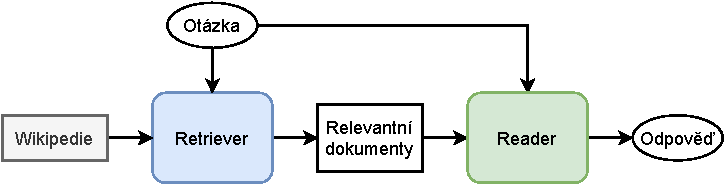
\includegraphics{obrazky/reader-retriever-scheme.pdf}
	}
	\caption{Generické schéma (prezentované například v~\cite{drQA}) open-domain QA systému}
	\label{qa_scheme}
\end{figure}

%=========================================================================
\section{Zvolený přístup k~problému}
Odpovídání na otázky na otevřené doméně (open-domain QA) má obvykle dvě hlavní (na sobě téměř nezávislé) části, jak je naznačeno na obrázku \ref{qa_scheme}. První částí je \emph{Retriever}, který má za úkol získat z~internetu (pro nás z~Wikipedie) relevantní dokumenty, které by mohly obsahovat odpověď a~druhou je \emph{Reader}, který provede extrakci odpovědi ze získaného kontextu \cite{drQA}.\par
\noindent\emph{Retriever} části systému je věnována pozornost v~sekci \ref{retriever_imp}.\par
Pro návrh systému bylo však největší dilema v~realizaci \emph{Reader} části systému pro kvalitní extrakci odpovědi v~češtině. Chtěl jsem využít některého z~populárních předtrénovaných modelů (\ref{bert_albert}) založených na Transformers \cite{Transformers} architektuře (\ref{transformers}). Proto jsem se rozhodl vyzkoušet přístup, kdy je nativně anglickému ALBERT modelu, který dosahuje špičkových výsledků\footnote{\url{https://rajpurkar.github.io/SQuAD-explorer/}}, strojově přeložen vstupní dokument i otázka z~češtiny do angličtiny.\par
Pro porovnání jsem zvolil vícejazyčný model BERTa (m-BERT\footnote{\url{https://github.com/google-research/bert/blob/master/multilingual.md} -- Zjednodušeně řečeno je to model BERT předtrénován na korpusech mnoha jazyků.}), který podporuje 104 světových jazyků s~nejrozsáhlejší Wikipedií, trénovaný na českém překladu datové sady SQuAD 1.1 \cite{czech_squad} \cite{squad}.\par

%=========================================================================
\section{Návrh jednotlivých částí systému}
\label{design}
V~této sekci bude popsán návrh systému, tedy hlavně \emph{Retrieveru}, \emph{Readeru} a~části pro zpracování datové sady SQAD v3.0 \cite{sqad} pro závěrečné vyhodnocení.

\subsection{Návrh Retrieveru}
Získání \emph{n} relevantních dokumentů kandidujících pro zodpovězení otázky vyžaduje několik na sebe navazujících kroků (obrázek \ref{retriever-simple-scheme}). V~návrhu a~implementaci jsou použity metody předzpracování textu a~řazení dokumentů popsané v~kapitolách \ref{text_processing} a~\ref{document_indexing}.\par
Retriever dostává na vstupu otázku, která je také hlavním vstupem do celého systému. Dříve, než se na základě otázky začnou přímo prohledávat odstavce české Wikipedii, bude dobré z~otázky získat co nejvíce informací, které by mohly vést ke \emph{spraveným článkům}. Až po jejich získání jsou jednotlivé články rozděleny na odstavce a~ty prohledávány.\par
\noindent K~získání článku jsou použity tři metody:
\begin{itemize}
    \item \textbf{základní Wiki Search} nezpracované otázky, který někdy přináší uspokojivé výsledky, ale většinou je nedostačující,
    \item \textbf{získání relevantního titulku článku} (pomocí BM25 \ref{bm25}) z~\emph{dumpu} titulků\footnote{\url{https://cs.wikipedia.org/wiki/Wikipedie:St\%C3\%A1hnut\%C3\%AD_datab\%C3\%A1ze}} a~abstraktů české Wikipedie po lemmatizaci otázky a~odstranění stop slov,
    \item \textbf{rozpoznání (pojmenované) entity}, která by se mohla vyskytovat v~titulku článku a~usnadnit tím \emph{Wiki Search}.
\end{itemize}
Tímto tedy získáme seznam článků z~Wikipedie, který je následně upraven tak, aby se v~něm každý získaný článek vyskytoval pouze jednou.\par
Jednotlivé články je následně třeba rozdělit na odstavce, normalizovat jejich délku, lemmatizovat je, odstranit stop slova a~indexovat je. Odstavce jsou poté seřazeny algoritmem BM25 a~z~nich vybrány první tři\footnote{V tomto případě pro účely experimentů -- nejúspěšnější varianta je vyhodnocena také s hodnotou 5 a 8.} nejvhodnější. Pro vyhledávání mezi odstavci je použita lemmatizovaná otázka s~odstraněnými stop slovy. Tři nejvhodnější odstavce jsou získány v~jejich původní, nezpracované podobě a~případně (při použití nativně anglického \emph{readeru}) jsou včetně otázky přeloženy do angličtiny.

\begin{figure}[hbt]
	\centering
	\scalebox{0.9}{
	    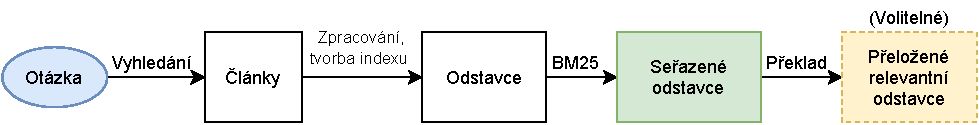
\includegraphics{obrazky/retriever-simple-scheme.pdf}
	}
	\caption{Zjednodušené schéma \emph{retriever} části systému}
	\label{retriever-simple-scheme}
\end{figure}

Následuje podrobný návrh struktury \emph{retrieveru} znázorňující podrobně jednotlivé komponenty na obrázku \ref{retriever-podrobne}.

\begin{figure}[hbt]
    \centering
	\scalebox{0.9}{
	    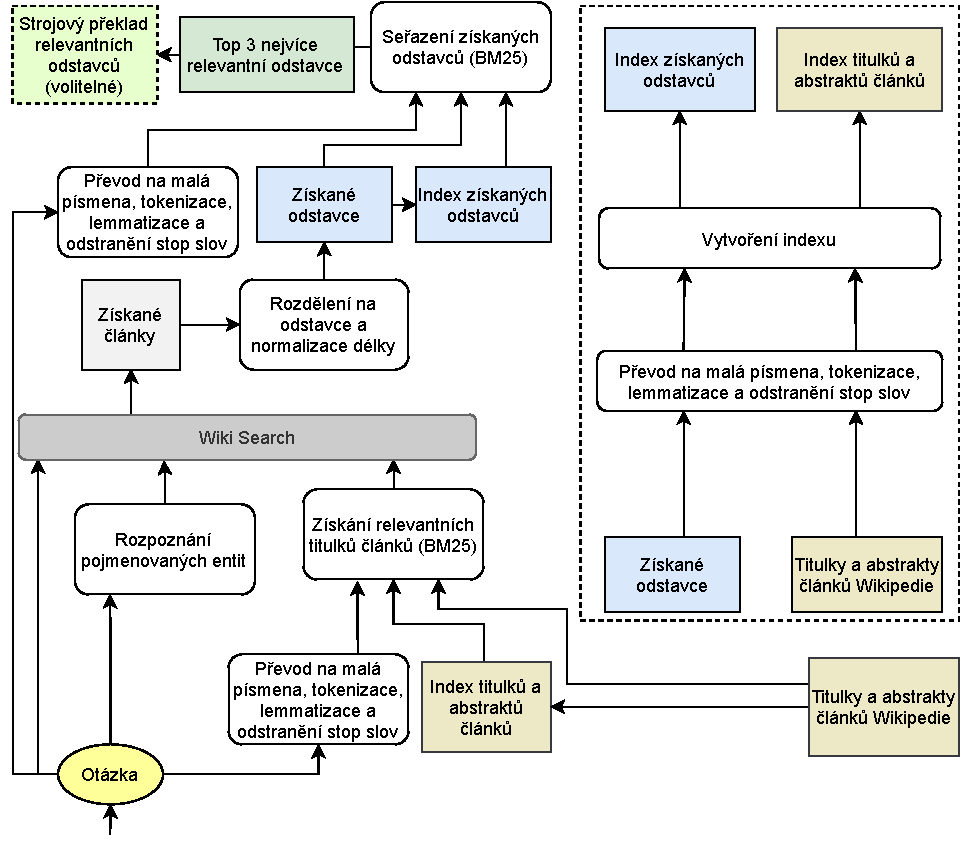
\includegraphics{obrazky/retriever_podrobne.pdf}
	}
	\caption{Podrobné schéma \emph{retriever} části systému}
	\label{retriever-podrobne}
\end{figure}

\subsection{Návrh Readeru}
Část systému pro extrakci odpovědi ze získaného dokumentu byla navržena ve dvou variantách.
\begin{itemize}
    \item \textbf{Anglický ALBERT} s~lineární klasifikační vrstvou pro určení začátku a~konce odpovědi, pro který jsou vstupní dokumenty a~otázka strojově přeloženy do angličtiny. Výsledná odpověď je přeložena opět zpět do češtiny.
    \item \textbf{Vícejazyčný BERT (m-BERT)} opět s~lineární klasifikační vrstvou pro určení začátku a~konce odpovědi, který dokáže odpovídat přímo na českých dokumentech.
\end{itemize}
Pro obě varianty je však postup (až na překlad pro anglický ALBERT, který je však součástí \emph{retrieveru}) shodný.\par
Model dostane k~přečtení tři nejvíce relevantní odstavce získané \emph{retrieverem}. Pro každý odstavec je provedena extrakce odpovědi, kdy je vybrána vždy právě jedna validní odpověď s~největším \uv{skóre}(nenormalizovaná logaritmická pravděpodobnost) pro daný dokument. Ze získaných odpovědí je vybrána ta, kterou si je model nejvíce jistý (ta s~největším skóre) a~případně (při použití ALBERT-en modelu) přeložena zpátky do češtiny.\par
\noindent Ostatní odpovědi jsou také uloženy pro získání statistických dat při vyhodnocení. \emph{Reader} tak vybere kromě odpovědi také finální dokument, ze kterého je odpověď získána, který může být použit pro získání některých dalších informací/kontextu uživatelem.\par
Schéma \emph{readeru} pro extrakci finální odpovědi je naznačeno na obrázku \ref{reader_schema}. Modely použité k~implementaci a~naznačeny v~návrhu byly blíže popsány v~kapitole \ref{language_comprehension}, konkrétně v~sekci \ref{bert_albert}.

\begin{figure}[hbt]
	\centering
	\scalebox{1.3}{
	    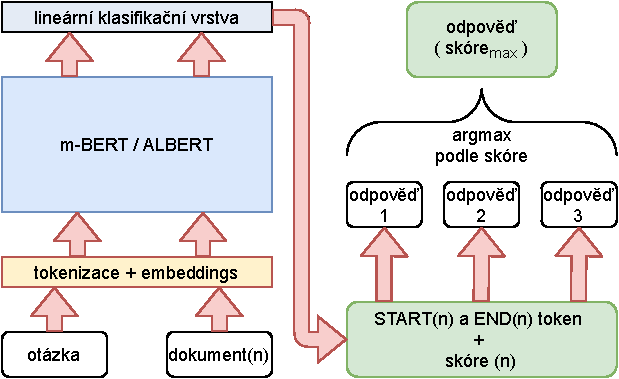
\includegraphics{obrazky/reader_navrh.pdf}
	}
	\caption{Schéma \emph{readeru} (kombinovaně pro oba navržené systémy) pro 3 relevantní dokumenty, kde $n \in (1,3)$. Pro model ALBERT by musel proběhnout ještě strojový překlad finální odpovědi do češtiny.}
	\label{reader_schema}
\end{figure}

\subsection{Návrh vyhodnocení}
Pro vyhodnocení byl vybrán český dataset SQAD v3.0, jak už bylo několikrát zmíněno. Pro vyhodnocení musely být navrženy metriky respektující charakteristiku datové sady i to, že se pohybujeme v~rámci otevřené domény. Kromě tradičních metrik EM (\emph{exact match}) a~F1 (popsány blíže v~kapitole \ref{metriky}) jsem se při návrhu vyhodnocení systému snažil respektovat několik věcí:
\begin{itemize}
    \item Kvůli otevřené doméně může být odpověď nalezena z~jiného kontextu v~jiném tvaru.
    \item Potřebujeme metriku pro ohodnocení samotného \emph{retrieveru} v~úspěšnosti nalezeného dokumentu.
    \item Metriku pro zohlednění i správných odpovědí, které byly nalezeny, i když nebyly například vybrány \emph{readerem} jako nejvhodnější.
\end{itemize}
Pro podrobnější popis zvolených metrik viz \ref{metriky}. Metriky budou použity pro porovnání systému využívající dva navržené přístupy v \emph{reader} části a~také aspektů ovlivňující \emph{retriever}.

\section{Existující systémy pro otevřenou doménu}
\label{existing_work}
Příkladem existujícího systému pro QA na otevřené doméně může být třeba dříve zmíněný článek \cite{drQA} (DrQA) prezentující \emph{retriever--reader framework}. Je poměrně jednoduchý a podobný navrženému systému v této práci. DrQA byl navržen pro odpovídání na otázky nad anglickou Wikipedií a jeho úspěšnost EM na datasetu SQuAD (1.1) je podle \cite{drQA} necelých 30\,\%.\par
Novější implementací může být například systém R2-D2 \cite{fajcik2021pruning}, který patřil k nejvíce úspěšným systémům soutěže NeurIPS 2020 \cite{min2021neurips}. R2-D2, neboli \textit{Rank twice -- Read twice}, používá architekturu sestávající ze čtyř částí: \emph{retriever, reranker, }extraktivní a generativní \emph{reader}. Retriever používá DPR \cite{dpr}(popsáno v části \ref{dpr}) a reranker využívá enkodér transformer architektury. Jeho úspěšnost na datasetu NQ (Natural Questions) dosahuje 55\%\,EM. V zásadě jsou si state of the art systémy v architektuře retriever\,--\,reader velmi podobné, s drobnými odchylkami (jako je reranker, extraktivní/generativní reader). Implementace R2--D2 se navíc snaží omezit paměťovou náročnost modelu. Pro modely bez omezení dosahuje úspěšnost těch nejlepších (v extrakci odpovědi) více jak 60\%\,F1 skóre\footnote{\url{https://ai.google.com/research/NaturalQuestions/leaderboard}}.\par\medskip
Pro češtinu existuje systém AQA (Automatic Question Answering) poprvé prezentován v práci \cite{aqa} a od té doby zdokonalován. Práce \cite{aqa} poskytující jakýsi benchmark pro evaluaci systému na otevřené doméně pro dataset SQAD (v1.0) je z roku 2016. Pozdější vyhodnocení pro zdokonalený systém a dataset SQAD v1.1 z roku 2018 je v článku \cite{aqa2018}. Výsledky systému vyhodnoceného v roce 2018 jsou shrnuty v tabulce \ref{tab:aqa_benchmark}. Novější vyhodnocení systému fungujícím na otevřené doméně architektury retriever\,--\,reader pro dataset SQAD 3.0 není k dispozici.
\begin{table}[H]
\centering
    \begin{tabular}{|l|l|c|}
    \hline
    \multicolumn{1}{|c|}{{\textbf{AQA}}} & EM    & \multicolumn{1}{l|}{počet testovacích vzorků} \\ \hline
    \textbf{SQAD v1.0}                       & 49,83 & 3301                                         \\ \hline
    \textbf{SQAD v1.1}                       & 38,08 & 3301                                         \\ \hline
    \end{tabular}
\caption{Úspěšnost systému AQA v přesné shodě s referenční odpovědí na datových sadách SQAD 1.0 a 1.1.}
\label{tab:aqa_benchmark}
\end{table}

\chapter{Implementace a~použité technologie}
\label{chapter:implementace}
Obsahem této kapitoly je popis použitých nástrojů a~implementace jednotlivých částí systému. Je popsáno jak a~pomocí jakých knihoven byl návrh z kapitoly \ref{chapter:design_} realizován a~jaké problémy bylo potřeba vyřešit. Rozebrán je taky postup zpracování dat potřebných pro funkci systému i jeho vyhodnocení.

%=========================================================================
\section{Použité nástroje a~technologie pro implementaci}
\label{pouzite_nastroje}
V této sekci budou popsány použité technologie a~knihovny použité při implementaci výsledného systému.\par
Pro implementaci byl vybrán jazyk \textbf{Python} (3.7.10), který nabízí největší množství knihoven a~nástrojů vhodných pro realizaci systému. Zároveň je vhodný ke zpracování dat a~je sympatický svou jednoduchou syntaxí. Nabízí také prostředí \emph{Jupyter notebook}, který je velmi pohodlný pro vývoj.\par
Některé knihovny implementují poznatky popsané v kapitolách \ref{text_processing}, \ref{language_comprehension} a~\ref{document_indexing}. Knihovny běžného charakteru, jako je například \texttt{json}, ve výčtu nejsou uvedeny.

\begin{itemize}
    \item \textbf{PyTorch}\footnote{\url{https://pytorch.org/}}
    je open-source framework pro strojové učení, zejména pro zpracování obrazu a~přirozeného jazyka. \par
    Nabízí implementace mnohých druhů neuronových sítí a~tensorových operací s GPU akcelerací (CUDA).
    
    \item \textbf{HuggingFace -- Transformers}\footnote{\url{https://huggingface.co/transformers/}}
    je populární (open-source) implementací nejznámějších Transformers architektur jako BERT nebo ALBERT (dále RoBERTa, XLM \dots) vyvinuta společností HuggingFace.\par
    Nabízí nástroje pro jednoduchou práci s modely, předzpracování jejich vstupu, trénink atd. Pro implementace modelů obecného využití jako BERT nabízí také jejich verze pro konkrétní úlohy, jako je odpovídání na otázky (extrakce odpovědi). Pro každou architekturu je k dispozici typicky několik předtrénovaných verzí (BERT base, BERT large \dots).\par
    Je implementována jak pro PyTorch, tak i pro velmi podobný framework TensorFlow\footnote{\url{https://tensorflow.org/}}.
    
    \item \textbf{HuggingFace -- Datasets}\footnote{\url{https://huggingface.co/docs/datasets/}}
    umožňuje snadnou práci s veřejně dostupnými datasety. Usnadňuje jejich načtení a~efektivní předzpracování.\par 
    Díky dostupnosti zdrojových kódů Umožňuje také úpravu skriptu pro načtení datové sady pro načtení jiné, která doposud v oficiálním seznamu knihovny není dostupná.
    
    \item \textbf{DeepPavlov}\footnote{\url{https://deeppavlov.ai/}}
    je open-source framework, postavený na Pytorch, TensorFlow a~Keras, pro usnadnění vývoje a~výzkumu v oblasti zpracování přirozeného jazyka, konkrétně dialogových systémů.
    
    \item \textbf{Rank-bm25}\footnote{\url{https://github.com/dorianbrown/rank\_bm25}}
    je knihovnou implementující hodnotící algoritmy z rodiny BM25 \cite{bm25_improvements} (Okapi, BM25+, BM25L).\par
    Nabízí velmi jednoduché API pro indexaci a~řazení dokumentů.
    
    \item \textbf{NumPy}\footnote{\url{https://numpy.org/}}
    nabízí jako knihovna velmi efektivní operace pro práci s vektory a~maticemi a~vícerozměrnými poli. Je nabízena pod licencí BSD (open-source).
    
    \item \textbf{NLTK}\footnote{\url{https://www.nltk.org/}}
    (Natural Language Toolkit) je open-source knihovna nabízející nástroje pro zpracování textu a~přirozeného jazyka.\par Prostřednictvím jednoduchého API umožňuje tokenizaci (včetně dělení na věty), stematizaci, tagování částí textu a~jiné. 
    
    \item \textbf{MorphoDiTa\footnote{\url{https://ufal.mff.cuni.cz/morphodita}} (corpy)\footnote{\url{https://corpy.readthedocs.io/en/stable/api/morphodita.html}}}
    je open-source nástrojem pro morfologickou analýzu umožnující například tokenizaci nebo lemmatizaci textu.\par
    Pro použití je potřeba také natrénovaný jazykový model, který je nabízený na webových stránkách v poznámce pod čarou pro češtinu a~angličtinu. Jednoduché API pro práci s MorphoDiTou nabízí knihovna \textbf{corpy}.
    
    \item \textbf{Majka}\footnote{\url{https://nlp.fi.muni.cz/czech-morphology-analyser/}}
    je podobně jako MorphoDiTa morfologickým analyzátorem.\par Majka provádí analýzu za použití morfologických slovníků. Slovníky jsou dostupné pro celou řadu jazyků, jako je čeština, slovenština, polština, angličtina, \dots
    
    \item \textbf{Wikipedia (api)}\footnote{\url{https://github.com/goldsmith/Wikipedia}}
    je knihovna usnadňující vyhledávání, získávání a~parsování článků z Wikipedie. \par Nabízí velmi jednoduché API pro vyhledávání článků a~získávání jejich textového obsahu.
    
    \item \textbf{Googletrans}\footnote{\url{https://github.com/ssut/py-googletrans}}
    nabízí API pro přístup k funkcionalitě Překladače Google. \par
    Je neoficiální implementací přístupu k překladači a~kvůli omezením na množství překládaných znaků nezajišťuje naprosto stabilní funkčnost.
    
    \item \textbf{Jupyter Notebook}\footnote{\url{https://jupyter.org/}} 
    je open-source webová aplikace pro interaktivní spouštění Python kódu v tzv. buňkách.\par
    Kromě zrojového kódu umožňuje také vkládání textu, vizualizaci dat, vkládání obrázků a~grafů nebo spouštění BASH (Shell) skriptů.
    
    \item \textbf{Google Colab}\footnote{\url{https://colab.research.google.com/notebooks/intro.ipynb}}
    je služba nabízející přístup k virtuálnímu stroji, který zprostředkovává přístup k Jupyter Notebooku v cloudu.\par 
    Virtuální stroje nabízí (bez rozšířené placené verze) asi 12\,GB RAM, úložiště s možností připojení a~přístup k Google Drive a~výkonné GPU s pamětí 16\,GB vhodné pro akceleraci výpočtů. Dokonce jsou dostupné i běhová prostředí s TPU pro paralelizaci výpočtů.\par
    Běhová prostředí vždy disponují množstvím předinstalovaných, běžně používaných knihoven (PyTorch, TensorFlow a~další).
    
\end{itemize}

%=========================================================================
\section{Zpracování dat v práci}
\label{data_processing}
Následující sekce popisuje, jak byla zpracována data, se kterými se v práci pracuje. \par
\noindent Nejprve je popsáno zpracování datasetu SQuAD a~jeho českého překladu, na kterých je trénován \emph{reader}. Poté je popsáno zpracování dumpů obsahující titulky a~abstrakty článků české Wikipedie. Vysvětleno je také zpracování českého datasetu SQAD v3.0 a~také formát uložení odpovědí při vyhodnocení testování systému, aby na nich mohla být provedena evaluace. 

\subsection{Předzpracování datové sady SQuAD}
Pro načtení datasetu SQuAD byla použita knihovna Huggingface \texttt{ datasets }, která načte trénovací i dev dataset dostupný ve formátu JSON. Pro načtení je použit skript \emph{squad.py}, který lze díky open-source povaze knihovny upravit a~použít i pro načtení české verze datasetu SQuAD \cite{cz_suqad_download} (skripty \emph{czech\_squad.py} a~\emph{czech\_squad2.py}). Stejně jednoduchý postup lze použít i pro načtení verze 2.0 obou datasetů.\par
Po načtení obsahuje dataset položku \emph{train} a~\emph{validation} pro trénink a~vyhodnocení natrénovaného modelu pro extrakci odpovědi. Velikosti jednotlivých částí jsou zmíněny v tabulce \ref{tab:squad_size_new}. Každá otázka ve SQuAD datasetu obsauje id, titulek, kontext(dokument), otázku a~odpověď. Odpovědí může být i více, pro odpověď je také uveden index znaku, na kterém začíná.\par
Z knihovny \texttt{transformers} je poté potřeba načíst tokenizér, který převede otázku a~kontext každé položky v datasetu do podoby stravitelné modelem (tokeny reprezentovány token ID pro předtrénovaný slovník modelu a~speciální tokeny jako [CLS] a~[SEP]). Pro více\-jazyčný BERT lze použít \texttt{BertTokenizerFast}, pro ALBERT zas \texttt{AlbertTokenizerFast}.\par
\pagebreak
Modely BERT a~ALBERT založené na Transformer architektuře mají pevně danou maximální délku vstupní sekvence tokenů. Proto je potřeba tokenizér nastavit tak, aby byly příliš dlouhé vstupy rozděleny na sekvenci kratších, ideálně s nějakým přesahem za sebou následujích oddělených částí (\texttt{return\_overflowing\_tokens=True}).\par
Při práci s odpovědí je v datasetu vyznačen pouze index počátečního znaku. Nastavením tokenizéru \texttt{return\_offsets\_mapping=True} získáme pro každý token také indexy vstupního řetězce znaků, na kterých se nachází.\par
S použitím popsaných metod jsou k původnímu datasetu přidány informace o indexu \emph{počátečního a~koncového tokenu} každé odpovědi pro daný tokenizér daného modelu.\par 
Funkce, která zpracování implementuje, byla vypůjčena z HuggingFace notebooku\footnote{\url{https://colab.research.google.com/github/huggingface/notebooks/blob/master/}} a~pomocí metody datasetu \texttt{map()} je aplikována na všechny vzorky datasetu.

\subsection{Práce s dumpem Wikipedie}
V práci byly použity dva různé soubory pro získání relevantních článků Wikipedie. Prvním je dump názvů článků a~druhým je dump abstraktů.\par
Soubor s názvy článků je pouze jednoduchý text snadný pro zpracování. Na každý řádek souboru připadá jeden název článku. Před vytvořením indexu je tedy třeba pouze nahradit podtržítka v názvech mezerou a~uložit názvy jednotlivých článků do seznamu.\par
Pro abstrakty článků je to o něco složitější, protože jsou uloženy v poměrně rozměrném XML souboru. Každý záznam obsahuje titulek, url, text abstraktu a~odkazy. Po načtení je dump zpracován tak, že je ponechána pouze informace o názvu článku a~text jeho abstraktu. Výsledný zpracovaný dump je uložen jako soubor JSON s asi čtvrtinovou velikostí souboru původního. Získání a~zpracování konkrétních článků je popsáno až v sekci \ref{retriever_imp}.

\subsection{Extrakce informací z datasetu SQAD}
Dataset SQAD v3.0 \cite{sqad_download} je dostupný ve velmi specifické struktuře. Jednotlivé otázky datové sady jsou rozesety po $13,476$ složkách, z nichž každá obsahuje 7\,--\,9 souborů \uv{vert}. Důležité pro nás jsou pouze soubory obsahující otázku a~extrakci odpovědi. Na obrázku \ref{question_format} je příklad formátu, ve kterém jsou otázky a~odpovědi uloženy. 

\begin{figure}[hbt]
	\centering
	\scalebox{0.3}{
	    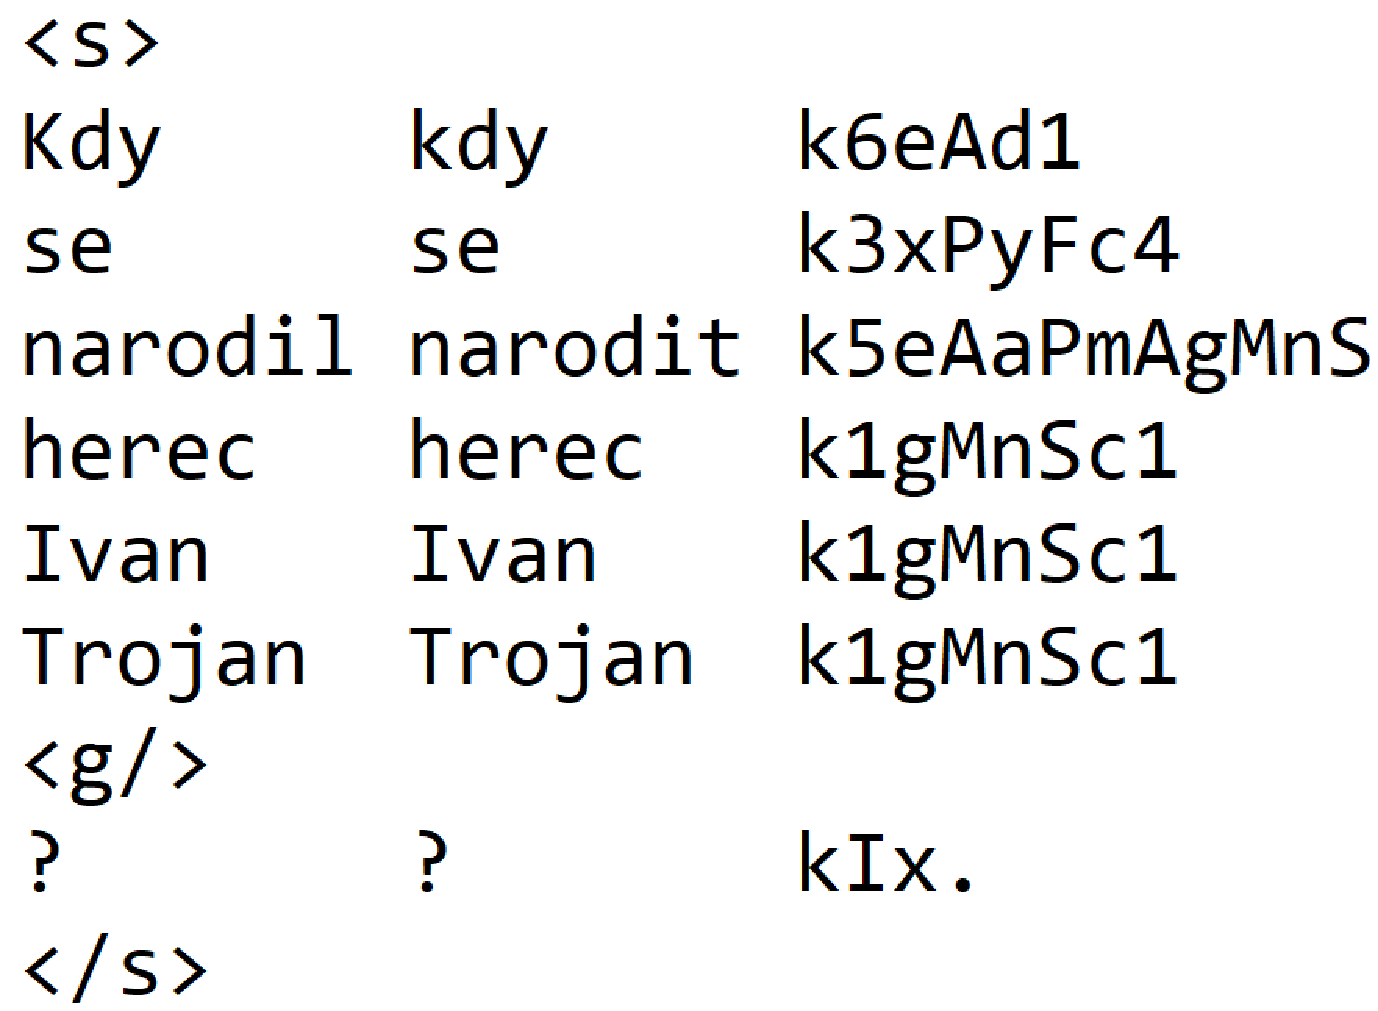
\includegraphics{obrazky/sqad_question_format.pdf}
	}
	\caption{Příklad formátu položky (otázky) datasetu SQAD v3.0.}
	\label{question_format}
\end{figure}

Pro každý záznam musí být tedy otevřeny a~zpracovány soubory obsahující otázku a~odpověď. První sloupec souboru obsahuje na každém řádku \emph{token} otázky/odpovědi, druhý sloupec jejich lemmata. Při zpracování je také potřeba brát ohled na speciální znaky.\par
Pro každý záznam je při zpracování uložena otázka, extrakce odpovědi a~lamma extrakce odpovědi. Záznamy obsahující \uv{ano/ne} odpovědi byly ze zpracování vynechány. Zpracovaný dataset je uložen ve formátu JSON (obr. \ref{fig:sqad_processed}) pro jeho pozdější snadnější a~rychlejší zpracování.

\begin{figure}[hbt]
	\centering
	\scalebox{0.35}{
	    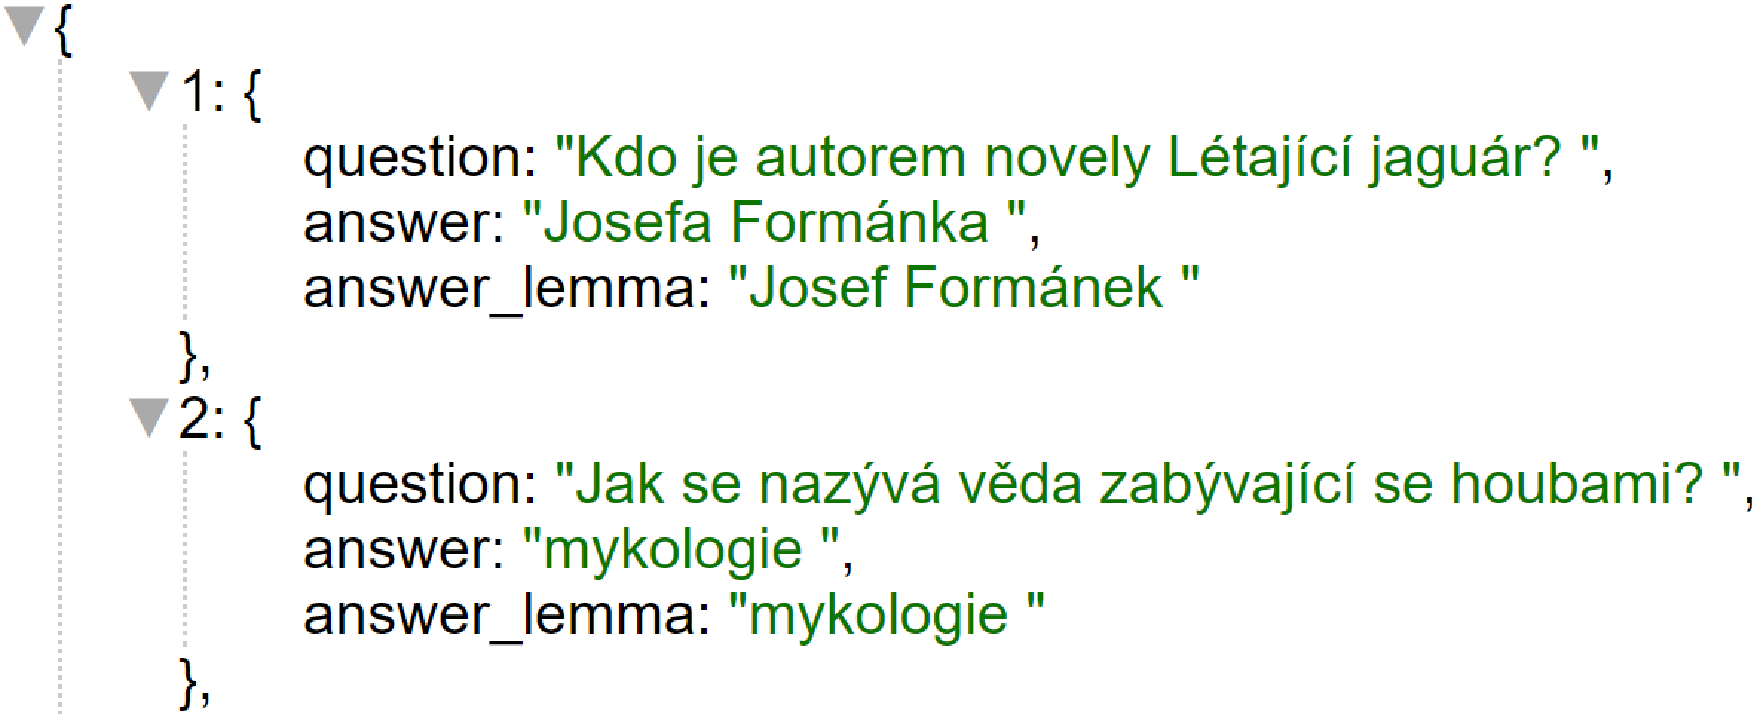
\includegraphics{obrazky/sqad_processed_format.pdf}
	}
	\caption{Příklad formátu JSON zpracovaného datasetu SQAD v3.0.}
	\label{fig:sqad_processed}
\end{figure}
%===========================================================================

\subsection{Ukládání dat pro vyhodnocení systému}
Pro uložení výsledků byl opět zvolen formát JSON, aby mohla být evaluace provedena až po získání odpovědí.\par
\begin{figure}[hbt]
	\centering
	\scalebox{0.4}{
	    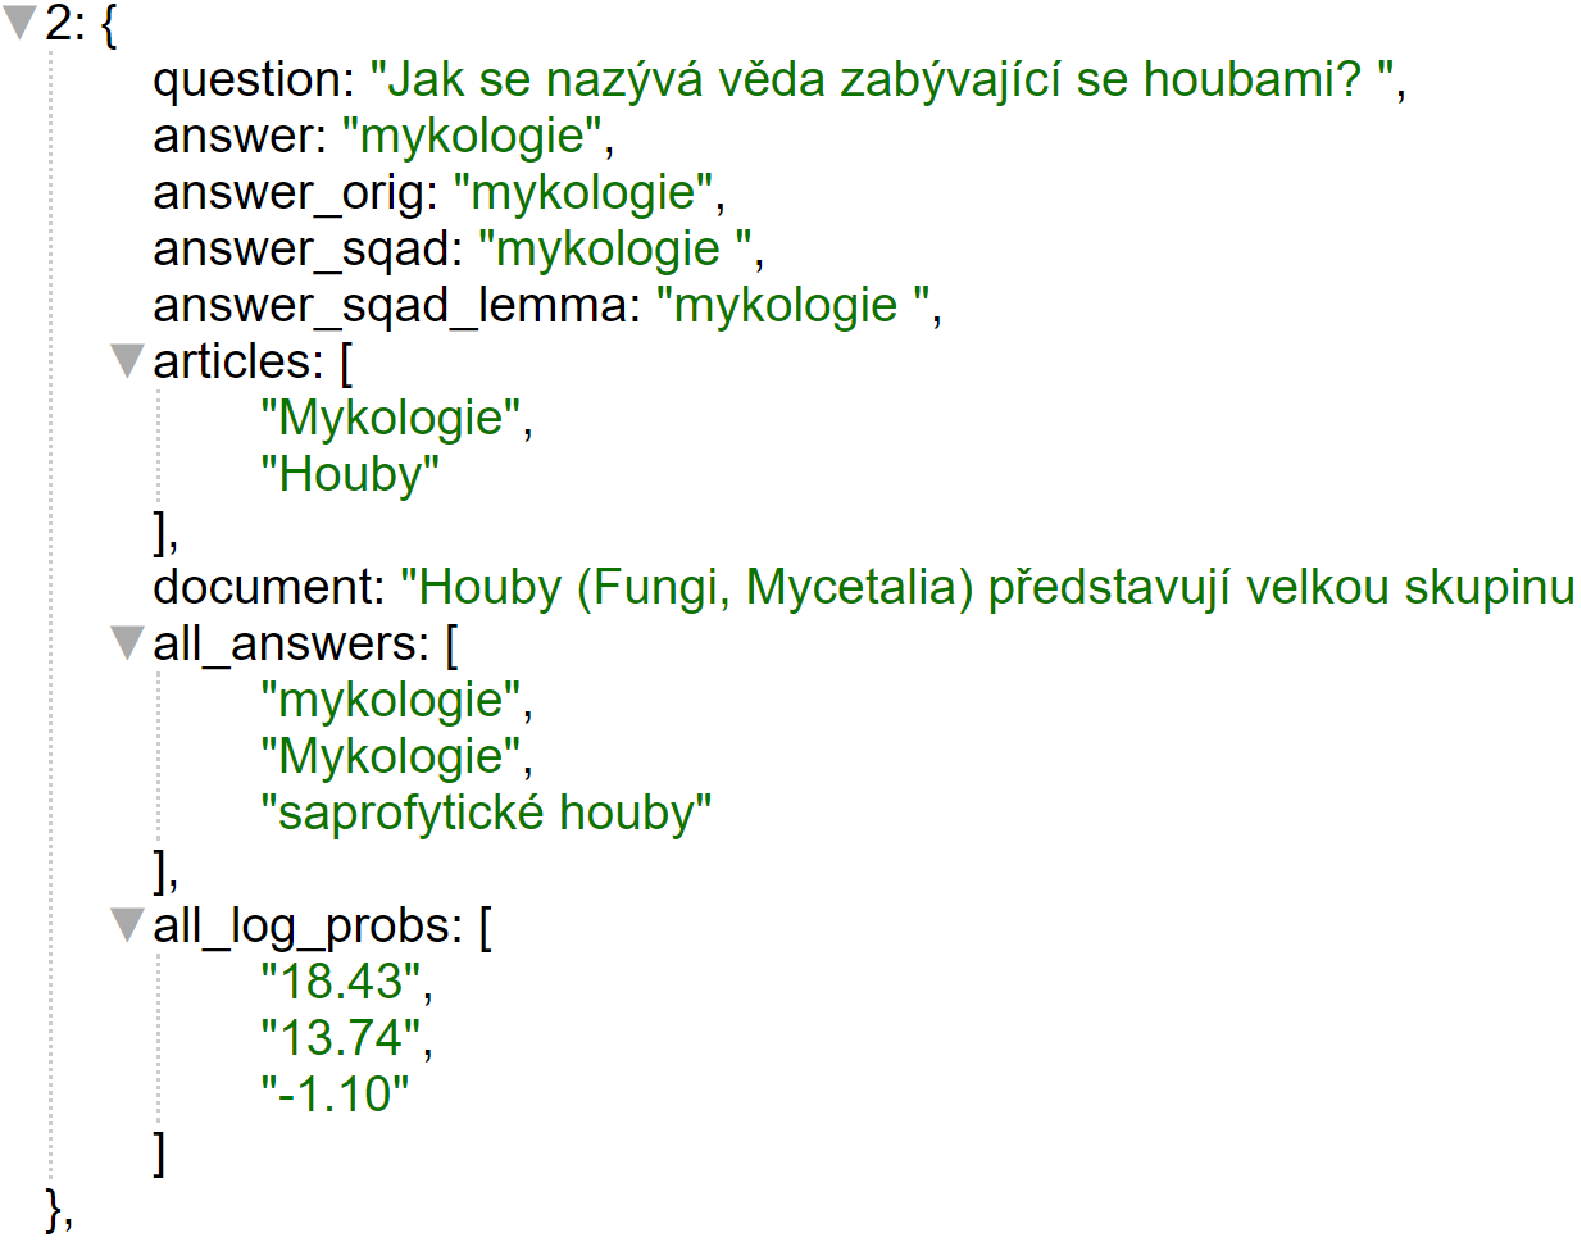
\includegraphics{obrazky/answer_saved_format.pdf}
	}
	\caption{Příklad formátu JSON uložené odpovědi s doplňkovými informacemi.}
	\label{fig:saved_answer}
\end{figure}
Pro každý zodpovězený záznam je uloženo číslo otázky \uv{2}, otázka \emph{question}, odpověď \emph{answer}, originální nepřeložená odpověď \emph{answer\_orig} (při použití m-BERT modelu, jako v příkladu, shodná s \emph{answer}), extrakce odpovědi podle datasetu SQAD \emph{answer\_sqad} a~její lemma \emph{answer\_sqad\_lemma}. Dále jsou pro podrobnější analýzu výsledků k dispozici názvy článků \emph{articles}, ve kterých systém odpověď vyhledával, kontext \emph{document}, ze kterého byla finální odpověď vybrána, první tři nejlepší odpovědi \emph{all\_answers} a~(nenormalizované) pravděpodobnosti \emph{all\_log\_probs} jednotlivých odpovědí z \emph{all\_answers}.\par
Soubor zodpovězených záznamů je pak pojmenován podle toho, jaký rozsah otázek obsahuje a~přidáno je i časové razítko.
\begin{center}
    answers\_1-3000\_\_04-04-2021\_09:53.json
\end{center}

%=========================================================================
\section{Implementace a~trénink readeru}
\label{reader_imp}
Pro implementaci \emph{readeru} systému byla použita knihovna\texttt{ transformers } od HuggingFace, která nabízí velmi jednoduché rozhraní pro trénink modelů.\par

\subsection{Trénink}
Pro trénink ALBERT modelu byla použita třída \texttt{ AlbertForQuestionAnswering } a~předtrénovaný model \texttt{albert-base-v2\footnote{\url{https://huggingface.co/albert-base-v2}} }(11 milionů parametrů). Model není příliš velký a dosahuje podobných výsledků, jako jeho větší verze \texttt{large} nebo \texttt{xlarge}. Pro \emph{fine-tuning} byl použit dataset SQuAD 1.1 a 2.0.\par
Pro druhý model byl použit\texttt{ BertForQuestionAnswering } z knihovny\texttt{ transformers.} Předtrénovaný model\texttt{ bert-base-multilingual-cased\footnote{\url{https://huggingface.co/bert-base-multilingual-cased}} } (110 milionů parametrů). Pro fine-tuning byl použit český překlad datasetu SQuAD 1.1 a 2.0. Pro načtení obou datasetů byl použit upravený skript \emph{squad.py}.\par
Všechny modely byly trénovány pomocí třídy\texttt{ Trainer }s následujícími parametry:
\begin{itemize}
    \item \emph{batch size} (velikost dávky) -- $16$
    \item \emph{learning rate} (rychlost učení) -- $2e\!-\!5$
    \item \emph{weight decay} -- $0,01$
    \item \emph{počet trénovacích epoch} -- $3$
\end{itemize}

Po \emph{fine-tuningu} je úspěšnost modelů (F1 a EM, viz \ref{metriky}) na jejich validačních datasetech následující (tabulka \ref{tab:reader_trained}). Oba modely byly trénovány na GPU ve službě Google Colab.

\begin{table}[h]
\centering
    \begin{tabular}{| l | l | l |}
        \hline
        \textbf{ALBERT} & SQuAD 1.1 & SQuAD 2.0 \\ \hline
        EM              & 82,14      & 78,33      \\ \hline
        F1              & 89,58      & 81,55      \\ \hline
    \end{tabular}
    \begin{tabular}{| l | l | l |}
        \hline
        \textbf{mBERT} & cz\_SQuAD 1.1 & cz\_SQuAD 2.0 \\ \hline
        EM              & 68,52      & 66,47      \\ \hline
        F1              & 77,72      & 69,54      \\ \hline
    \end{tabular}
    \caption{
    Úspěšnost modelů na validačních datasetech.
    }
    \label{tab:reader_trained}
\end{table}

\subsection{Extrakce odpovědi}
Třída zajišťující extrakci odpovědi se nazývá \texttt{Reader}. Pro extrakci odpovědi z kontextu je nejprve potřeba vytvořit její instanci. Většina parametrů pro inicializaci jsou volitelné, musíme však zadat cestu k natrénovanému modelu (\texttt{model\_checkpoint}) v úložišti a jeho typ (\texttt{model\_type}). Můžeme také upravit maximální délku odpovědi (\texttt{max\_answer\_length}) a maximální počet validních odpovědí (\texttt{n\_best\_size}), které model vybere. \emph{Reader} načte tokenizér a model, který bude pro extrakci odpovědi využívat a použije GPU, pokud je k dispozici.\par
Pro extrakci odpovědi je poté možné volat jedinou instanční metodu \texttt{get\_answers}, která vyžaduje otázku s kontextem a vrací pole o velikosti \texttt{n\_best\_size} obsahující nejlepší kandidáty pro odpověď. Každá odpověď se skládá z textu "text" a skóre "score".\par
Pro každý dokument je poté vybrána nejlépe hodnocená odpověď s neprázdným textem.

%=========================================================================
\section{Implementace retrieveru}
\label{retriever_imp}
Pro získání relevantních dokumentů je implementována třída \texttt{Retriever}. Pro její inicializaci je třeba zadat cestu k modelu (\texttt{dita\_file}) pro nástroj MorphoDiTa, který provádí lemmatizaci, cestu k souboru s titulky článků Wikipedie (\texttt{wiki\_titles}) a ke zpracovanému JSON souboru s abstrakty Wikipedie (\texttt{wiki\_abstracts}). Místo MorphoDiTy může \texttt{Retriever} použít i nástroj Majka (\texttt{majka=True}), pro který je potřeba zadat cestu k souboru s morfologickým slovníkem (\texttt{majka\_file}). Pokud není k dispozici zpracovaný soubor s abstrakty, lze původní dump abstraktů převést na formátovaný JSON pomocí funkce \texttt{parse\_abstracts()}.\par
Při vytváření instance \texttt{Readeru} je načten lemmatizátor, sestaven index titulků článků a index abstraktů článků Wikipedie, načten tokenizér (pro rozdělení textu na věty) a načten model pro rozpoznávání entit.\par

\paragraph{Použitá stop slova --}
Pokud je potřeba při zpracování textů v průběhu vyhledávání relevantního dokumentu odstranit stop slova, je pro to využit následující seznam\footnote{\scriptsize \url{https://cs.wiktionary.org/wiki/P\%C5\%99\%C3\%ADloha:Frekven\%C4\%8Dn\%C3\%AD\_seznam\_(\%C4\%8De\%C5\%A1tina)}}:
\begin{quote}
    {\footnotesize kdy být a se v na ten on že s z který mít do já o k i jeho ale svůj jako za moci pro tak po tento co když všechen už jak aby od nebo říci jeden jen můj jenž ty stát u muset chtít také až než ještě při jít pak před však ani vědět hodně podle další celý jiný mezi dát tady tam kde každý takový protože nic něco ne sám bez či dostat nějaký proto}
\end{quote}
Dále je k dispozici seznam pro odstranění interpunkce:
\begin{quote}
    {\footnotesize . , ? ! ... " ( ) ; - /}
\end{quote}

\paragraph{Tvorba indexu --}
Pro vytvoření indexu pro prohledávání je použita třída \texttt{BM25Okapi} z dříve zmíněné knihovny \texttt{rank-bm25}. Každý titulek/abstrakt je převeden na malá písmena, lemmatizován a poté jsou z něj odstraněny stop slova. Získány jsou zpracované tokeny každého titulku/abstraktu. Index titulků/abstraktů je poté vytvořen pomocí \texttt{BM25Okapi} z takto zpracovaných titulků/abstraktů.

\paragraph{Rozpoznání pojmenovaných entit --}
Rozpoznání pojmenovaných entit (NER - \emph{Named Entity Recognition}) je další úloha na poli NLP. Uveďme alespoň příklad jejího použití:
\begin{center}
    Kdy vynalezl Alfred Nobel dynamit? $\longrightarrow$ Alfred Nobel
\end{center}
NER může usnadnit vyznačení klíčových slov pro vyhledávání.\par
Pro rozpoznání pojmenované entity v otázce je použita knihovna \texttt{deeppavlov}. Využívá natrénovaný model \texttt{ner\_ontonotes\_bert\_mult}, který je vytvořen funkcí \texttt{build\_model()}.

\subsection{Získání relevantních dokumentů}
Inicializace třídy \texttt{Retriever} trvá hlavně kvůli tvorbě indexů a načtení modelu pro NER poměrně dlouho\footnote{Asi 10 minut, pokud není potřeba stáhnout \texttt{deeppavlov} model pro NER. Pokud lze načíst vytvořený model přes \texttt{pickle}, může to být pouze kolem jedné minuty.}. Po jeho inicializaci je potřeba pro získání relevantních dokumentů pouze jediná instanční metoda \texttt{retrieve()}, která pro zadanou otázku získá $n$ (v práci 3) relevantních dokumentů.\par
Získání dokumentů probíhá následovně:
\begin{enumerate}
    \item Nejprve jsou získány názvy článků metodou \texttt{get\_doc\_list()}, které jsou výsledkem vyhledávání metody \texttt{search()} knihovny \texttt{wikipedia}. Jednotlivé vstupy do vyhledávání jsou následující:
    \begin{itemize}
        \item V otázce jsou rozpoznány pojmenované entity
        \item Otázka je převedena na malá písmena, lemmatizována a jsou z ní odstraněny stop slova.
        \begin{itemize}
            \item Pomocí metody vytvořeného indexu titulků \texttt{get\_top\_n()} je získán nejvíce relevantní titulek článku vzhledem k otázce.
            \item Pomocí metody vytvořeného indexu abstraktů \texttt{get\_top\_n()} je získán nejvíce relevantní titulek článku vzhledem k otázce.
        \end{itemize}
        \item Otázka je pro vyhledání použita nezpracovaná.
    \end{itemize}
    Pokud jsou některé výsledky vyhledávání stejné, je použit pouze jeden z nich.
    
    \item Pro každý získaný název článku je získán jeho textový obsah metodou \texttt{page()} kni\-hovny \texttt{wikipedia}. Ten je rozdělen na jednotlivé odstavce a jsou z něj odstraněny nepotřebné části jako reference a odkazy.
    
    \item Je zkontrolováno, jestli některý z odstavců nepřesahuje maximální délku. Je-li potřeba odstavec dále rozdělit, je použita metoda \texttt{normalize\_length()}, která využívá tokenizéru knihovny \texttt{nltk}. Ten rozdělí odstavec na věty a spojuje jednotlivé věty, dokud není dosaženo maximální délky. Pro zbývající věty je vytvořen další odstavec, který obsahuje také poslední 2 věty odstavce předcházejícího.
    
    \item Po normalizaci délky získaných odstavců je potřeba získat jejich zpracovanou verzi, aby mohl být sestaven index pro vyhledávání. Každý odstavec je tedy převeden na malá písmena, lemmatizován a jsou z něj odstraněna stop slova (a interpunkce). Pro každý odstavec je získán seznam takto normalizovaných tokenů, které jsou použity pro tvorbu indexu \texttt{BM25Okapi} pro vyhledávání.
    
    \item Původní lemmatizovaná otázka převedená na malá písmena bez stop slov je použita pro vyhledávání v indexu získaných odstavců pomocí metody \texttt{get\_top\_n()}. Tím jsou získány (nezpracované\footnote{Zpracování probíhá pouze pro tvorbu indexu.}) nejvíce relevantní odstavce -- dokumenty pro danou otázku.
\end{enumerate}
\pagebreak
\section*{Nalezení odpovědi na otázku}
Celý tok programu systémem je následující:
\begin{itemize}
    \item Je vytvořena instance třídy pro extrakci odpovědi \texttt{Reader}, instance třídy pro získání relevantních dokumentů \texttt{Retriever} a také instance překladače \texttt{Translator} knihovny \texttt{googletrans}.
    
    \item Po zadání otázky je volána funkce \texttt{find\_answer()}, která získá odpověď na otázku.
    \begin{itemize}
        \item Pomocí \emph{retrieveru} jsou získány relevantní dokumenty
        \item V případě použití nativně anglického modelu ALBERT jsou dokumenty spolu s otázkou přeloženy pomocí funkce \texttt{transtale()} do angličtiny.
        \item Pro každý získaný dokument je provedena extrakce odpovědi a vybrána nejlépe ohodnocená neprázdná odpověď.
        \item Ze získaných extrakcí odpovědi z jednotlivých dokumentů je vybrána ta, která má nejvyšší skóre. Použita je metoda \texttt{argmax()} knihovny \texttt{numpy}. Pomocí získaného indexu je vybrán dokument i odpověď.
        \item Vybraná odpověď je při použití anglického modelu pro extrakci přeložena zpět do češtiny.
        \item Funkce vrací odpověď. Pro podrobné vyhodnocení dále: (odpověď před překladem), dokument, ve kterém byla odpověď nalezena, seznam nejlepších odpovědí, seznam skóre nejlepších odpovědí, seznam sum skóre nejlepších odpovědí, seznam článků Wikipedie, které byly pro nalezení odpovědi procházeny a seznam nejlepších dokumentů, které byly pro nalezení odpovědi přečteny.
    \end{itemize}
\end{itemize}


%=========================================================================
%===============================================================================

\chapter{Vyhodnocení systému a~rozbor chyb}
\label{system_evaluation}
V této kapitole jsou popsány výsledky dosažené vytvořeným systémem. Popsán je vliv použitého přístupu pro \emph{reader}, trénovacího datasetu a použitého nástroje pro morfologickou analýzu. Nejprve jsou popsány standardní i speciální metriky, na nichž je úspěšnost systému prezentována. Výsledky jsou poté porovnány s jiným existujícím řešením. Jsou diskutovány hlavní nedostatky a příčiny chyb a možnosti dalšího zlepšení.


%=========================================================================
\section{Vysvětlení základních metrik}
\label{metriky}
V této sekci jsou popsány metriky použité pro vyhodnocení systému. Popsány jsou standardní metriky jako EM a F1 používané pro QA systémy a také metriky zachycující specifika otevřené domény.\par
Metody EM a F1 (používané např. pro vyhodnocení na \cite{squad}, \cite{squad_v2}), MRR (např. pro~\cite{sqad}) a částečně T3M jsou standardní metriky používané pro vyhodnocení většiny podobných systémů. Ostatní metriky jsou úpravou těch standardních, navržené specificky pro vyhodnocení tohoto systému.

\subsection{Exact Match (EM)}
\label{EM}
\emph{Exact match}, neboli přesná shoda, je jednoduchá standardní metrika, které ale může diskriminovat dostačující odpovědi s pouze malými rozdíly oproti referenčním výsledkům. Její hodnota může být buď 1 (pokud je shoda dosažena) nebo 0 (pokud se oproti referenční hodnotě výsledek liší, byť jen v jednom znaku). Na příkladu je ukázka penalizace odpovědi, která byla dokonce přesnější, než referenční odpověď.\par
\begin{center}
\begin{tabular}{l}
    \textbf{otázka:} Kde se narodil Gabriel Jonas Lippmann?\\
    \emph{referenční odpověď:} Bonnevoie\\
    \emph{odpověď systému 1:} Bonnevoie, Lucembursko -- \textbf{EM} -- 0\\
    \emph{odpověď systému 2:} Bonnevoie -- \textbf{EM}-- 1
\end{tabular}
\end{center}
Pro vyhodnocování je referenční i získaná odpověď převedena před porovnáním na malá písmena. Při vyhodnocování systému s readerem ALBERT je brána v úvahu i původní, nepřeložená odpověď.

\subsection{Exact Lemma Match (ELM)}
\label{ELM}
ELM je speciálně navržená metrika pro toleranci drobných rozdílů oproti referenční odpovědi. Kromě převedení na malá písmena jsou odpovědi před porovnáním také lemmatizovány. Skóre ELM je tedy typicky vyšší, než EM.
\begin{center}
\begin{tabular}{l}
    \textbf{otázka:} Kdy se koná dostihový závod Velká pardubická?\\
    \emph{referenční odpověď:} druhou říjnovou neděli\\
    \emph{odpověď systému:} druhá říjnová neděle \\
    \textbf{EM} -- 0 , \textbf{ELM} -- 1\\
\end{tabular}
\end{center}

Skóre ELM nabývá opět hodnoty buď 1 (správně) nebo 0 (špatně), stejně jako pro EM. ELM pro příklad uvedený v \ref{EM} by bylo také 0.

\subsection{Naivní skóre (NS)}
Naivní skóre je nejvíce benevolentní metrikou. Zjišťuji u ní, zda-li je odpověď nebo její lemma podřetězcem referenční odpovědi nebo jejího lemma, případně naopak. Snaha je tedy zachytit co nejvíce alespoň částečně správných odpovědí. Naivní skóre (NS) příkladu uvedeného v podsekci \ref{EM} nebo \ref{ELM} by tedy bylo 1. 

\subsection{Top 3 Match (T3M)}
T3M je obdobou EM \ref{EM}, pro shodu je však testována každá z nejlepších třech (3) nalezených odpovědí. Můžeme tedy určit, v kolika případech oproti EM systém našel správnou odpověď, ale nevybral ji, protože nedosáhla nejvyššího skóre. T3M nabývá opět hodnoty 0 nebo 1.

\subsection{MRR}
MRR (\emph{Mean Reciprocal Rank}) je obdobou T3M, zohledňuje však, na kolikátém místě byla odpověď nalezena (T3M zohledňuje pouze to, jestli byla vůbec nalezena). Pokud dosáhla odpověď shodná s referenční odpovědí nejvyšší skóre (byla vybrána), hodnota MRR je 1, pokud byla na druhém místě, hodnota je 1/2 a pokud na třetím, hodnota MRR je 1/3. Pokud nebyla odpověď nalezena vůbec, hodnota MRR je 0 \cite{MRR}.

\subsection{F1 skóre}
Je jakýmsi kompromisem mezi naivním skóre a EM. Při jeho výpočtu jsou použity dvě metriky --- \emph{recall} (úplnost) a \emph{precision} (přesnost) \cite{information_retrieval}.
\begin{equation}
    \text{\textbf{F1}} = 2\cdot \frac{precision \cdot recall}{precision + recall} 
\end{equation}
\begin{equation}
recall = \frac{tp}{tp+fn} \quad precision = \frac{tp}{tp+fp}
\end{equation}

\begin{itemize}
    \item tp -- \emph{true positive} -- znaky (počet) společné pro zíkanou i referenční odpoěď
    \item fn -- \emph{false negative} -- znaky, které jsou v referenční odpovědi, ale chybí v získané
    \item fp -- \emph{false positive} -- znaky, které nejsou v referenční odpovědi, ale přebývají v získané
\end{itemize}

Obvykle jsou definice tp, fn a fp uváděny pro tokeny, ne znaky, chceme ale více zohlednit morfologii češtiny a dropné rozdíli v odpovědích vztahující se k otevřené doméně -- například augustiánský/augustiánských -- při porovnávání tokenů bychom nedosáhli žádné shody. F1 skóre je počítáno, pouze pokud je získaná odpověď podřetězcem té referenční, nebo naopak.\par \medskip
\noindent Pro příklad: 
\begin{center}
\begin{tabular}{l}
    \textbf{otázka:} Odkud byla anglická kapela The Beatles?\\
    \emph{referenční odpověď:} z Liverpoolu\\
    \emph{odpověď systému:} Liverpoolu\\
\end{tabular}
\end{center}
je tedy $precision = 1$, $recall = 0,83$ a $\text{\textbf{F1}} = 0,91$.\par \medskip
\noindent Pro příklad z \ref{EM}
\begin{center}
\begin{tabular}{l}
    \textbf{otázka:} Kde se narodil Gabriel Jonas Lippmann?\\
    \emph{referenční odpověď:} Bonnevoie\\
    \emph{odpověď systému:} Bonnevoie, Lucembursko\\
\end{tabular}
\end{center}
je $precision = 0,41$, $recall = 1$ a $\text{\textbf{F1}} = 0,82$.\par \medskip
F1 tedy zohledňuje přesnost i úplnost odpovědi a je velmi směrodatnou metrikou pro odpovídání na otázky.

\subsection{Lidské vyhodnocení}
Otevřená doména je problematická pro automatické vyhodnocování. Jak je uvedeno například v \cite{min2021neurips}, otázka může mít více možných odpovědí, pokud není jednoznačně položena. Odpověď může být také obecnější, nebo specifičtější (př. z \ref{EM}), ale stále odpovídat na otázku. Z článku \cite{min2021neurips} tedy vyplývá, že systémy jsou hodnoceny lépe při vyhodnocení lidmi. Konkrétně, procento odpovědí označených jako \uv{rozhodně správně} bylo u systémů v průměru o 17\,--\,25\,\% lepší, než pouhé porovnání řetězců odpovědí pomocí EM.\par
Proto je pro každý experiment také náhodně vybráno 200 otázek pro lidské vyhodnocení, aby se vzal alespoň minimální ohled na diskriminační povahu automatické evaluace.

%=========================================================================
\section{Vyhodnocení výsledného open-domain systému}
Pro vyhodnocení celého systému byla vybrána datová sada SQAD v3.0 \cite{sqad}, ze které byly odebrány ano/ne otázky.\par
Pro každou metriku v \ref{metriky} bylo použito vzorce \ref{score_calc}
\begin{equation}
    \label{score_calc}
    \text{skóre} = \frac{1}{N}\cdot \sum^N_{k=1} S_k
\end{equation}
kde $S_k$ je skóre $S$ (např. EM) pro odpověď $k$ a $N$ je celkový počet odpovědí. Skóre na celém datasetu je tedy průměrem jednotlivých skóre $S_k$ všech zodpovězených otázek.\par
V této sekci jsou shrnuty a porovnány výsledky výsledného systému na testovací sadě.\par
Pro každou variantu systému bylo provedeno vyhodnocení pouze na (stejné) čtvrtině\footnote{Velikost čtvrtiny datasetu je \textbf{2819 vzorků} -- srovnatelné s počtem vzorků při vyhodnocení AQA v \cite{aqa2018}.} datasetu, která byla získána tak, že byl vybrán každý jeho čtvrtý vzorek. Pro vítěznou variantu bylo vyhodnocení provedeno na všech více jak 11000 vzorcích a byly provedeny další experimenty.

\subsection{Model ALBERT a strojový překlad}
\label{albert_eval}
Vyhodnocení systému s readerem ALBERT, pro který jsou nalezené texty strojově překládány do angličtiny. Vyhodnocení proběhlo pro 4 varianty -- reader trénován na datasetu SQuAD 1.1/2.0 (SQ1.1/2.0) a nástroj použitý pro morfologickou analýzu -- Majka/MorphoDiTa (Maj/MD). Nejlepší výsledky a důležité metriky jako EM a F1 jsou zvýrazněny tučně.

\begin{table}[H]
    \centering
    \begin{tabular}{|l||l|l|l|l|l|l|l|l|l|}
        \hline
        \textbf{ALBERT}  & \textbf{EM}   & ELM       & NS        & T3M       & MRR       & \textbf{F1}   & prec.         & rec. \\ \hline\hline
            SQ1.1+MD    & 11,96         & 25,63     & 37,77     & 23,61     & 21,17     & 22,93         & 21,80         & 25,81    \\ \hline
            SQ2.0+MD    & 12,85         & 26,08     & 39,57     & 23,63     & 21,66     & 23,87         & 22,77         & 26,80    \\ \hline
            SQ1.1+Maj   & 11,64         & 25,37     & 37,90     & \textbf{23,78}     & 21,40     & 23,03         & 21,88         & 25,98    \\ \hline
            SQ2.0+Maj   & \textbf{12,88}& \textbf{26,15}& \textbf{39,60}& 23,60     & \textbf{21,68}     & \textbf{24,11}         & \textbf{22,98}         & \textbf{27,09}    \\ \hline
    \end{tabular}
    \caption{Úspěšnost [\%] systému s readerem ALBERT a strojovým překladem textů -- vyhodnoceno pro čtvrtinu datasetu SQAD v3.0 (2819 otázek).}
    \label{tab:system_eval_albert}
\end{table}
Jak je vidět v tabulce \ref{tab:system_eval_albert}, výsledky tohoto přístupu nejsou příliš dobré. Za povšimnutí stojí výrazný rozdíl mezi EM a ELM. Příčinou tak velké odchylky od přesné shody je nejspíš ztráta tvaru slov při překladu, kdy však slovní základ zůstává stejný. Naivní skóre dosahuje téměř 40\%, nějaké shody tedy systém dosáhl, ale nepřesnosti způsobené překladem převládly.

\subsection{Model vícejazyčný BERT}
\label{mbert_eval}
Vyhodnocení systému používajícího vícejazyčný BERT jako reader. Vyhodnocení proběhlo opět ve 4 variantách stejně jak v předchozí podsekci \ref{albert_eval}. Značení je stejné s jediným rozdílem, kdy SQ1.1/2.0 jsou českými strojovými překlady datové sady SQuAD použité pro trénink readeru. Nejlepší výsledky jsou opět zvýrazněny tučně.

\begin{table}[H]
    \centering
    \begin{tabular}{|l||l|l|l|l|l|l|l|l|l|}
        \hline
        \textbf{mBERT}  & \textbf{EM}   & ELM       & NS        & T3M       & MRR       & \textbf{F1}   & prec.         & rec.      \\ \hline\hline
            SQ1.1+MD    & 41,22         & 43,17     & 59,67     & 46,68     & 43,73     & 52,31         & 54,77         & 53,07     \\ \hline
            SQ2.0+MD    & \textbf{42,85}&\textbf{44,84}&\textbf{61,83}&\textbf{47,11}&\textbf{44,80}&\textbf{54,33}&\textbf{56,94}&\textbf{55,04}\\ \hline
            SQ1.1+Maj   & 40,90         & 42,85     & 59,13     & 46,29     & 43,38     & 51,79         & 54,27         & 52,55         \\ \hline
            SQ2.0+Maj   & 42,36         & 44,38     & 61,16     & 46,65     & 44,32     & 53,63         & 56,26         & 54,35     \\ \hline
    \end{tabular}
    \caption{Úspěšnost [\%] systému s readerem m-BERT trénovaném na čekém překladu datasetu SQuAD -- vyhodnoceno pro čtvrtinu datasetu SQAD v3.0 (2819 otázek).}
    \label{tab:system_eval_mbert}
\end{table}

Při použití vícejazyčného modelu BERT bylo dosaženo poměrně uspokojujících výsledků (tab. \ref{tab:system_eval_mbert})a jeho nejlepší varianta je tedy dále vyhodnocena na všech 11273 otázkách testovací datové sady.\par
Následuje ještě ale podsekce o ručním vyhodnocení lidmi, která zachycuje diskriminační povahu automatických metrik.\pagebreak

\subsection{Vyhodnocení člověkem}
\label{human_eval}
Z celé datové sady SQAD v3.0 bylo náhodně vybráno 200 otázek, které byly vyhodnoceny také ručně -- lidmi (inspirováno \cite{min2021neurips}). Porovnáno na nich bude tedy úspěšnost jednotlivých systémů dle automatického vyhodnocení\footnote{U tohoto vzorku a lidských hodnotitelů jsou pro porovnání vybrány pouze metriky EM a F1.} a vyhodnocení lidmi, jinak řečeno, jestli by danou odpověď systému bral člověk jako postačující.\par
Následující tabulka \ref{tab:human_eval} prezentuje přehledně zjištěné hodnoty.

\begin{table}[H]
\centering
\begin{tabular}{|l||l|l|l|}
    \hline
        {ALBERT}       & \textbf{EM} & \textbf{F1} & \textbf{člověk} \\ \hline\hline
    SQ1.1+MD  & 11,00       & 24,46       & 55,50               \\ \hline
    SQ2.0+MD  & 11,00       & 24,48       & 54,50               \\ \hline
    SQ1.1+Maj & 11,00       & 24,48      & \textbf{56,50}               \\ \hline
    SQ2.0+Maj & \textbf{12,00}       & \textbf{24,92}      & 53,50               \\ \hline
    \end{tabular}
    \begin{tabular}{|l||l|l|l|}
    \hline
    {mBERT}       & \textbf{EM} & \textbf{F1} & \textbf{člověk} \\ \hline\hline
    SQ1.1+MD  & 43,00       & 53,15         & 64,00               \\ \hline
    SQ2.0+MD  & \textbf{46,00}& \textbf{56,81}& \textbf{69,00}              \\ \hline
    SQ1.1+Maj & 42,00       & 52,55           & 63,00               \\ \hline
    SQ2.0+Maj & 45,00       & 56,21           & 67,50               \\ \hline
    \end{tabular}
\caption{Porovnání automatického vyhodnocení a vyhodnocení lidmi systémů vyhodnocených v \ref{albert_eval} a \ref{mbert_eval} na 200 náhodně vybraných otázkách.}
\label{tab:human_eval}
\end{table}

Při tomto vyhodnocení byla odpověď ohodnocena 1, pokud byla při ručním vyhodnocení odpověď systému dostačující odpovědí na danou otázku a 0 v opačném případě. U výsledků je vidět rozdíl mezi přesnou shodou a lidským vyhodnocením až 45,5\,\% u~systému využívajícího strojový překlad a reader ALBERT a až 23\,\% u systému využívajícího vícejazyčný BERT.\par
Výsledky tedy indikují použitelnost odpovědi téměř 70\,\% u nejlepší varianty systému. Také ukazují mnohem větší použitelnost výsledků prvního přístupu, než se při prvotním vyhodnocení mohlo zdát, avšak nedosahují kvalit systému využívajícího vícejazyčný BERT.\par
Pro ilustraci je uvedeno pár příkladů, které byly při ručním vyhodnocení posouzeny jako dostačující:

\begin{table}[H]
\centering
\begin{tabular}{|l|l|}
\hline
\textbf{č.}   &\textbf{Otázka}                                         \\ \hline
1               &Kolik má čeština slovních druhů?                        \\ \hline
2                &Kdo je Oldřich Homuta?                                  \\ \hline
3                &Která diecéze má jako hlavní patronku svatou Zdislavu?  \\ \hline
4                &Jaké je jméno současného papeže?                        \\ \hline
5                &Kdo je vrchním velitelem ozbrojených sil ČR?            \\ \hline
6                & Kde zemřel Platón?                                      \\ \hline
\end{tabular}
\begin{tabular}{|l|l|l|}
\hline
\textbf{č.}   &\textbf{Odpověď systému} & \textbf{Referenční odpověď} \\ \hline
1               &deset                    & 10                          \\ \hline
2               &český elektrotechnik     & vynálezce remosky           \\ \hline
3               &litoměřické diecéze      & litoměřický                 \\ \hline
4               &kardinál Bergoglio       & František                   \\ \hline
5               &Miloš Zeman              & prezident České republiky   \\ \hline
6               &Atény                    & v Athénách                  \\ \hline
\end{tabular}
\caption{Příklady odpovědí systému (různých variant z vyhodnocovaných), které byly posouzeny člověkem jako dostačující.}
\label{tab:human_eval_examples}
\end{table}

\subsection{Porovnání dosažených výsledků}
Vyhodnocení jednotlivých variant systému proběhlo v předchozích podsekcích a můžou být tedy shrnuty závěry experimentů. \par
Pro variantu ALBERT došlo oproti variantě mBERT pouze k velmi malé přesné shodě získaných výsledků. Pro obě varianty systému byl úspěšnější \emph{reader} trénovaný na verzi 2.0 datasetu SQuAD, tedy na tom, který pro trénink obsahuje i velké množství dokumentů neobsahujících odpověď na položenou otázku. Tento trénink nejspíš přispěl k o něco lepšímu průměru výběru správného dokumentu.\par
Co se týká lexikálních analyzátorů a jejich vliv na funkci hodnotící funkce \texttt{bm25}, zvítězil v první variantě analyzátor Majka, ne však příliš přesvědčivě a procentuální rozdíl úspěšnosti systému je téměř zanedbatelný. Pro druhou variantu zvítězil analyzátor MorphoDiTa a o něco přesvědčivěji. Ve všech experimentech byl však rozdíl v systémech používajících různý lexikální analyzátor téměř zanedbatelný. Kvůli tomu, že byl však ve druhé (úspěšnější) variantě nástroj MorphoDiTa systematicky (byť jen o trochu) lepší, je použit pro vyhodnocení systému na celé testovací datové sadě právě on.\par
Co se týká ručního vyhodnocení lidmi, byly všechny varianty mnohem úspěšnější, než podle automatického vyhodnocení. Větší rozdíl mezi automatickým a lidským vyhodnocení byl zaznamenán u první varianty systému s readerem ALBERT, kde jsou odpovědi deformovány opakovaným překladem textu do angličtiny a zpět do češtiny. Reálná použitelnost této varianty systému však není tak špatná, jak se z automatického vyhodnocení zdá.\par
Z provedených experimentů je tedy vítěznou variantou systém mBERT SQ2.0+MD. Tedy systém používající jako reader vícejazyčný BERT natrénovaný na českém překladu datasetu SQuAD 2.0 a nástrojem MorphoDiTa pro morfologickou analýzu.

\subsection{Vyhodnocení nejlepšího dosaženého systému}
\label{best_eval}
V této části jsou uvedeny výsledky vyhodnocení nejlepší varianty systému na celém datasetu SQAD 3.0. Experimentováno bylo s množstvím dokumentů, které jsou předány readeru k extrakci odpovědi. V tabulce \ref{tab:final_evaluation} jsou uvedeny výsledky vyhodnocení systému.
\begin{table}[H]
    \centering
    \begin{tabular}{|l||l|l|l|l|l|l|l|l|l|}
        \hline
          & \textbf{EM}   & ELM       & NS        & TkM       & MRR       & \textbf{F1}   & prec.         & rec. \\ \hline\hline
            top 3    & 42,30         & 44,21     & 61,20     & 46,67     & 44,27     & 53,69         & 56,12         & 54,44    \\ \hline
            top 5    & 43,71         & 45,64     & 62,80     & 50,02     & 46,41     & 55,20         & 57,62         & 55,95    \\ \hline
            top 8   & \textbf{43,89}         & \textbf{45,83}     & \textbf{62,96}     & 52,36     & 47,34     & \textbf{55,42}         & \textbf{57,70}         & \textbf{56,28}    \\ \hline
            top 10   & 43,77         & 45,68     & 62,87     & \textbf{53,07}     & \textbf{47,48}     & 55,28         & 57,52        & 56,17    \\ \hline
    \end{tabular}
    \caption{Vyhodnocení systému [\%] na celém datasetu SQAD 3.0 (bez ano/ne otázek --~viz tabulka \ref{tab:sqad_size}) s~využitím Wikipedie jako báze znalostí. Porovnáno je množství čtených dokumentů \uv{top~\emph{k}}. TkM je varianta metriky T3M (\ref{metriky}) pro každou variantu top \emph{k} čtených dokumentů. Varianta systému: extraktivní reader -- vícejazyčný BERT trénován na datasetu cz\_SQuAD 2.0 (\ref{reader_imp}), morfologický analyzátor -- MorphoDiTa.}
    \label{tab:final_evaluation}
\end{table}
Při vyhodnocení na celé testovací sadě se hodnoty od výsledků na čtvrtině datasetu v podsekci \ref{mbert_eval} o mnoho neliší. Z tabulky \ref{tab:final_evaluation} vyplývá, že nejlepší pro maximalizaci skóre EM i většiny dalších je čtení 8 nejvíce relevantních dokumentů. Při hodnotě 10 už úspěšnost většiny metrik klesla. Zvýšilo se však skóre TkM i MRR, což je s větším množstvím získaných dokumentů očekávatelné.

%=========================================================================
\section*{Porovnání výsledků práce se současným stavem poznání}
V této sekci jsou výsledky práce porovnány s podobnými systémy stejného účelu, pro které je dostupné vyhodnocení na standardních metrikách.\par
\begin{table}[H]
\centering
\begin{tabular}{|l|l|l||l|l|}
\hline
Systém     & dataset   & počet testovacích otázek & \textbf{EM} & \textbf{NS} \\ \hline \hline
AQA 2018   & SQAD v1.0 & 3 301                    & 49,83       & 59.58       \\ \hline
AQA 2018   & SQAD v1.1 & 3 301                    & 38,08       & 46,26       \\ \hline
\textbf{Tato práce} & SQAD v3.0 & 11 273                   & 43,89       & 62,96       \\ \hline
\end{tabular}
\caption{Porovnání výsledků této práce se systémem AQA \cite{aqa} (uvedené výsledky jsou převzaty z \cite{aqa2018}). Výsledky jsou uvedeny v \%.}
\label{tab:aqa_compare}
\end{table}
Výsledky práce jsou porovnány s výsledky systému AQA \cite{aqa}, konkrétně s poslední dostupnou vyhodnocenou variantou tohoto systému z roku 2018 \cite{aqa2018}, která byla vyhodnocena na 3301 otázkách z datasetu SQAD v1.0 a 1.1. Výsledky jsou shrnuty v tabulce \ref{tab:aqa_compare} a jsou porovnány pomocí metrik EM a NS. Metrika NS není v práci specifikována, pracuje se v~ní však s \uv{plnou shodou} (EM) a \uv{částečnou shodou}, která je definována jako odpověď, která se přesně neshoduje s referenční, protože některá slova přebývají, nebo chybí. \emph{Částečná shoda} uváděna při vyhodnocení systému AQA je tedy značena jako NS -- naivní skóre (viz \ref{metriky}), což je metrika této práce, která popisu nejvíce odpovídá. NS pro AQA je součtem hodnot \emph{plné} a \emph{částečné} shody uvedených v \cite{aqa2018}.\par
Z výsledků uvedených v tabulce \ref{tab:aqa_compare} je patrné, že systém AQA převyšuje výsledky této práce pouze v metrice EM a to pouze na části zastaralého datasetu SQAD v1.0. Z tabulky je patrné (a je tak uvedeno i v práci \cite{aqa2018}), že při vyhodnocení na stejně velkém vzorku vybraného z aktualizované verze datasetu 1.1, úspěšnost systému výrazně klesla (z EM 49,83\% na EM 38,08\%). Takový (možná i výraznější) pokles by šlo očekávat i při vyhodnocení systému na datasetu SQAD v3.0 použitého v této práci, která navíc vyhodnocuje systém na výrazně větším počtu vzorků. Systém prezentovaný v mé práci navíc dosahuje výrazně vyšších hodnot naivního skóre, které koresponduje s procentem použitelných výsledků více, než přesná shoda (jak je uvedeno v části \ref{human_eval}).\par
Výsledky práce tedy považuji ve srovnání s dostupným vyhodnocení systému AQA, který představuje relevantní porovnání s výsledky mé práce, za úspěch.\par
Výsledky mohou být porovnány také se \textit{state of the art} systémy, které však existují pouze pro angličtinu a jsou vyhodnoceny na datasetu NQ. Například v sekci \ref{existing_work} zmíněný systém R2--D2 (55\,\% EM), nebo nejlepší výsledky na datasetu NQ uvedené v jeho oficiálním žebříčku (až 64\,\% F1). Rozdílnost datasetu sice neposkytuje příliš validní porovnání, jsem však ale přesvědčen, že výsledky této práce takových kvalit nedosahují. Přesto si systém v porovnání s existujícími systémy nevede příliš špatně.


%=========================================================================
\section{Rozbor chyb a~možnosti dalšího vývoje}
V této sekci jsou rozebrány nedostatky systému, příčiny nesprávných odpovědí a možnosti vylepšení/nahrazení jeho existujících komponent pro optimální funkci systému. Navrhovaná vylepšení jsou zmíněna jak v krátkém, tak dlouhém časovém horizontu.\par
\subsection{Analýza chyb a jejich příčin}
Dataset je pro analýzu chyb nejprve rozdělen do 5 částí, které jsou vyhodnoceny samostatně. Z každé části jsou uloženy nesprávné odpovědi, které jsou nejblíže zkoumány pro část testovacích vzorků s nejnižší úspěšností. Úspěšnost na jednotlivých pěti částech je uvedena v tabulce \ref{tab:partial_eval}.

\begin{table}[H]
\centering
\begin{tabular}{|l|l|l|l|l|}
\hline
           & \textbf{EM} & \textbf{F1} & \textbf{NS} & \textbf{MRR} \\ \hline
\textbf{1} & 57,69       & 65,70       & 71,26       & 60,89        \\ \hline
\textbf{2} & 40,75       & \textbf{52,09}       & 59,69       & 44,61        \\ \hline
\textbf{3} & 41,65       & 53,57       & 61,54       & 44,89        \\ \hline
\textbf{4} & \textbf{38,70}       & 53,36       & 62,19       & \textbf{42,16}        \\ \hline
\textbf{5} & 40,68       & 52,38       & \textbf{60,07}       & 44,18        \\ \hline
\end{tabular}
\caption{Vyhodnocení systému na jednotlivých pětinách datasetu (1 -- 5), kde každá pětina má asi 2255 vzorků, pro první pětinu jsou tedy vyhodnoceny vzorky s číslem 1 až 2255. Tučně jsou uvedeny nejnižší hodnoty (v \%).}
\label{tab:partial_eval}
\end{table}

Nejlépe dopadla při vyhodnocení s velkým náskokem první část vyhodnocovací sady. Nejhůře část 4 (otázky 6765 -- 9020), kde přesná shoda nedosáhla 40\,\%. Pro tuto část je tedy proveden rozbor chyb. Pro rozbor byly vybrány vzorky, u kterých nebylo dosaženo přesné shody, nebo bylo dosažené F1 skóre méně, než 0,5. Získáno bylo tedy 982 vzorků pro bližší analýzu.\par
Prvním směrodatným údajem je skóre TkM -- tedy přesná shoda v alespoň jedné extrakci odpovědi, která byla pro přečtené dokumenty provedena. Hodnota tohoto skóre dosahuje 15,78\,\%. Tyto chyby jsou tedy způsobeny špatným výběrem získané odpovědi, která je závislá na skóre určeném \emph{readerem}.\par
Ze zbývajících 827 vzorků bylo dosaženo NS 13,66\,\%, což indikuje alespoň minimální použitelnost tohoto zlomku získaných odpovědí. Zbývá tedy zjistit příčinu chyb u 714 odpovědí, kde nebylo dosaženo žádné shody.\par
Pro zbývající vzorky bylo provedeno vyhodnocení, které má za úkol zjistit, jestli se referenční odpověď nachází v některém z top $n$ (kde pro analyzovaný systém $n=8$) dokumentů. Ta byla nalezena ve 37,11\,\% analyzovaných vzorků. Pro tyto shody bylo vypočítáno také skóre MRR 25,68\,\%, které zhodnocuje i pořadí relevance těchto dokumentů, ve kterém byly získány retrieverem.\par
Z původních 982 analyzovaných chybných vzorků můžeme tedy 533 považovat za chybnou extrakci odpovědi, nebo její špatné ohodnocení a vybrání nesprávné. Pro zbylých 449 vzorků nebyla správná odpověď nalezena v jediném získaném dokumentu. Vzhledem k původnímu vzorku pětiny datasetu (2255 zodpovězených otázek) je to tedy asi 20\,\%. Výsledky této analýzy prezentuje tabulka \ref{tab:error_analysis}.

\begin{table}[H]
\centering
\begin{tabular}{|l||c|c|c|}
\hline
\textbf{typ chyby}                & \multicolumn{1}{l|}{\textbf{zastoupení (v \%)}} & \multicolumn{1}{l|}{\textbf{počet}} & \multicolumn{1}{l|}{\textbf{původ chyby}}                                              \\ \hline
nevybrání správné odpovědi        & 15,78                                          & 155                                              & \multirow{3}{*}{reader (54\,\%)}                                                       \\ \cline{1-3}
nízká shoda s referenční odpovědí & 11,51                                          & 113                                              &                                                                                        \\ \cline{1-3}
chybná extrakce (nulová shoda)    & 26,99                                          & 265                                              &                                                                                        \\ \hline
nenalezení relevantního dokumentu & 35,95                                          & 353                                              & \multirow{2}{*}{\begin{tabular}[c]{@{}c@{}}retriever /\\ auto. vyhod.\end{tabular}} \\ \cline{1-3}
správná odpověď (ručně)           & 9,77                                           & 96                                               &                                                                                        \\ \hline
\end{tabular}
\caption{Příčiny chyb v analyzovaném vzorku 982 chybně zodpovězených otázek.}
\label{tab:error_analysis}
\end{table}

Pro otázky, které nebyly správně zodpovězeny a byly klasifikovány jako chyba retrieveru, protože nedošlo k nalezení relevantního dokumentu obsahujícího odpověď, bylo provedeno ruční vyhodnocení. V těchto 449 otázkách bylo nalezeno 96 odpovědí, které jsou při ručním vyhodnocení člověkem postačující. Zbylo tedy 353 vzorků a z ručního vyhodnocení vyplývá několik hlavních příčin chyb:
\begin{itemize}
    \item mnohoznačnost otázky/otázka nedává bez kontextu smysl
    \begin{itemize}
        \item \uv{Proč se Severu nedostávalo zkušených vojevůdců?}, \uv{Proč Franco zaútočil na severu?}, \uv{Co udělal Smith v roce 1999?}, \dots
    \end{itemize}
    \item správná odpověď se nachází mezi nevybranými, je však v jiném tvaru
    \item po převodu na malá písmena (viz \ref{retriever_imp}) se ztrácí část kontextu
    \item nebyly získány dostatečně relevantní dokumenty
    \item neschopnost readeru identifikovat ve složitém kontextu odpověď
\end{itemize}

\subsection{Další vývoj a možnosti navazujících prací}
Práce pokládá základ systému, který nabízí velký prostor pro další vylepšení. Návrhy toho, jak by mohlo být řešení rozšířeno například v rámci navazujících prací je popsáno v této části.\par
Nejdříve co se týká první části systému -- retrieveru pro získávání relevantních pasáží. Řazení pomocí hodnotící funkce BM25 by mohlo být nahrazeno modernějším přístupem DPR popisovaným v části \ref{dpr}, ať už za použití vícejazyčného BERTa, nebo jiného modelu (enkodéru) pro získání vektorové reprezentace. Pro získávání pasáží by oproti přístupu v této práci, kdy jsou procházeny pouze relevantní články, mohla být vhodně zpracována a indexována celá Wikipedie, případně by mohly být zpracovány i zvláštní struktury, jako tabulky, kde se často nachází spousta relevantních informací. Při zpracování textu by mohl být vylepšen také převod na malá písmena, aby nedocházelo ke ztrátám kontextu.\par
Co se týká modulu pro extrakci odpovědi, jsou cesty dalšího vývoje velmi otevřené. Prvním vylepšením by mohl být modul pro odhad předmětu otázky, aby došlo k lepší shodě při výběru odpovědi (otázka se ptá na datum -- uvažujme pouze odpovědi, které jsou také datum). Zajímavý by mohlo být také experimentovat s další variantou BERTa použitelného pro češtinu -- například Slavic BERT \cite{slavicBERT}. Mimo existující předtrénované ekodéry by měl být předmětem výzkumu hlavně předtrénink ryze české varianty například modelu ALBERT. Takový pokus již sice byl uskutečněn (například práce \cite{Zelina2020thesis}), model však nedosahoval dostatečných kvalit. Experimentovat by se dalo dále s přidáním abstraktivního readeru, jak je učiněno například v \cite{fajcik2021pruning}.\par
Přínosné by bylo také další rozšíření datasetu SQAD, nebo tvorba nového datasetu zaměřeného na otevřenou doménu, obsahující více reálných příkladů toho, na co se lidé ptají na internetu -- ať už pro trénink retrieveru (DPR), nebo pro reálnější vyhodnocení schopností takového systému.

%=========================================================================
%===============================================================================

\chapter{Závěr}
\label{conclusion}
Práce popisuje tvorbu systému schopného odpovídat na otázky nad českou Wikipedií.\par
Popisuje metody zpracování textu, strojového učení, modely vhodné pro porozumění textu a extrakci odpovědi a zhodnocuje také metody získávání relevantních pasáží. Popisuje dostupné aplikace popsaných postupů pro češtinu. Zhodnocuje dostupnost a vhodnost existujících datových sad pro trénink i vyhodnocení systému.\par
Po rozebrání teorie vztahující se k tématu je popsán návrh systému a jeho komponent. Popsány jsou použité nástroje a to, jak byl výsledný systém implementován. Práce poté prezentuje množství experimentů a variant systému a jejich podrobné vyhodnocení. Pro nejúspěšnější variantu je poté provedena evaluace na datasetu SQAD 3.0. Analyzovány jsou výsledky vyhodnocení, příčiny chyb i možnosti dalšího vývoje.\par
Podařilo se vytvořit systém, který splňuje požadavky zadání. Při řešení bylo experimentováno se dvěma přístupy -- použití anglického modelu ALBERT, pro který jsou pasáže strojově překládány a použití vícejazyčného modelu BERT. Oba systémy byly natrénovaný pro extrakci odpovědi. Porovnány byly také morfologické analyzátory MorphoDiTa a Majka a jejich vliv na získání relevantních pasáží.\par
Nejlépe se osvědčila varianta systému využívající vícejazyčný BERT trénovaný na českém překladu datasetu SQuAD 2.0 a využívající nástroj MorpoDiTa pro morfologickou analýzu. Tato varianta systému byla vyhodnocena na datasetu SQAD v3.0 (bez ano/ne odpovědí). Podařilo se vytvořit systém, který dosahuje úspěšnosti 43,89\,\% EM a 55,42\,\% F1 skóre a převyšuje výsledky systému AQA z roku 2018. Nastavuje také laťku pro další práce na podobných systémech.\par
Pro systém byla provedena analýza chyb a jejich příčin a také ruční vyhodnocení části chybně zodpovězených otázek. Ruční vyhodnocení nasvědčuje, že by mohla být reálná použitelnost odpovědí až o 23\,\% vyšší (až 69\,\%), než nasvědčuje metrika přesné shody EM. Pro systém využívající anglický model ALBERT je tento rozdíl mnohem větší (12,88\,\%EM, přes 50\,\% při lidském vyhodnocení), což je způsobeno deformací frází při opakovaném překladu pasáže/odpovědi. Diskutována jsou také úskalí použití datasetu SQAD pro vyhodnocení systému na otevřené doméně, jak ruční vyhodnocení nasvědčuje.\par
Další vývoj by mohl zahrnovat použití DPR pro hodnocení pasáží textu, zpracování a indexace celé Wikipedie, začlenění modulu pro klasifikaci otázek a odpovědí, trénink ryze českých kvalitních modelů jako je ALBERT či rozšíření existujících a tvorbu nových datasetů pro češtinu.
%%TODO vytvořit plakát

%=========================================================================
%===============================================================================

  \fi
  
  % Kompilace po částech (viz výše, nutno odkomentovat)
  % Compilation piecewise (see above, it is necessary to uncomment it)
  %\subfile{projekt-01-uvod-introduction}
  % ...
  %\subfile{chapters/projekt-05-conclusion}


  % Pouzita literatura / Bibliography
  % ----------------------------------------------
\ifslovak
  \makeatletter
  \def\@openbib@code{\addcontentsline{toc}{chapter}{Literatúra}}
  \makeatother
  \bibliographystyle{bib-styles/Pysny/skplain}
\else
  \ifczech
    \makeatletter
    \def\@openbib@code{\addcontentsline{toc}{chapter}{Literatura}}
    \makeatother
    \bibliographystyle{bib-styles/Pysny/czplain}
  \else 
    \makeatletter
    \def\@openbib@code{\addcontentsline{toc}{chapter}{Bibliography}}
    \makeatother
    \bibliographystyle{bib-styles/Pysny/enplain}
  %  \bibliographystyle{alpha}
  \fi
\fi
  \begin{flushleft}
  \bibliography{xsasin05-literatura}
  \end{flushleft}

  % vynechani stranky v oboustrannem rezimu
  % Skip the page in the two-sided mode
  \iftwoside
    \cleardoublepage
  \fi

  % Prilohy / Appendices
  % ---------------------------------------------
  \appendix
\ifczech
  \renewcommand{\appendixpagename}{Přílohy}
  \renewcommand{\appendixtocname}{Přílohy}
  \renewcommand{\appendixname}{Příloha}
\fi
\ifslovak
  \renewcommand{\appendixpagename}{Prílohy}
  \renewcommand{\appendixtocname}{Prílohy}
  \renewcommand{\appendixname}{Príloha}
\fi
%  \appendixpage

% vynechani stranky v oboustrannem rezimu
% Skip the page in the two-sided mode
%\iftwoside
%  \cleardoublepage
%\fi
  
\ifslovak
%  \section*{Zoznam príloh}
%  \addcontentsline{toc}{section}{Zoznam príloh}
\else
  \ifczech
%    \section*{Seznam příloh}
%    \addcontentsline{toc}{section}{Seznam příloh}
  \else
%    \section*{List of Appendices}
%    \addcontentsline{toc}{section}{List of Appendices}
  \fi
\fi
  \startcontents[chapters]
  \setlength{\parskip}{0pt} 
  % seznam příloh / list of appendices
  % \printcontents[chapters]{l}{0}{\setcounter{tocdepth}{2}}
  
  \ifODSAZ
    \setlength{\parskip}{0.5\bigskipamount}
  \else
    \setlength{\parskip}{0pt}
  \fi
  
  % vynechani stranky v oboustrannem rezimu
  \iftwoside
    \cleardoublepage
  \fi
  
  % Přílohy / Appendices
  \ifenglish
    \input{projekt-30-prilohy-appendices-en}
  \else
    % Tento soubor nahraďte vlastním souborem s přílohami (nadpisy níže jsou pouze pro příklad)

% Umístění obsahu paměťového média do příloh je vhodné konzultovat s vedoucím
\chapter{Obsah přiloženého paměťového média}

\dirtree{%
    .1 /. 
    .2 \textbf{benchmarks}/\DTcomment{odpovědi systému pro vyhodnocení}. 
        .3 všechny odpovědi systému z experimentů ve formátu json. 
    .2 \textbf{data/}\DTcomment{data potřebná pro experimenty a web server}. 
        .3 modely, zpracovaná data, \dots. 
    .2 \textbf{notebooks/}. 
        .3 question\_answering.ipynb\DTcomment{pro experimenty se systémem a zpracování dat}. 
        .3 mbert\_czech\_squad\_fine-tuning.ipynb\DTcomment{pro trénink mBERT modelů}. 
        .3 albert\_squad\_fine-tuning.ipynb\DTcomment{pro trénink ALBERT modelů}. 
        .3 czech\_squad.py. 
        .3 czech\_squad2.py\DTcomment{stažení datasetů pro trénink mBERT}. 
    .2 \textbf{poster.pdf}\DTcomment{plakát prezentující výsledky práce}. 
    .2 \textbf{readme.md}. 
    .2 \textbf{source\_tex/}\DTcomment{text práce v jeho zdrojové podobě}. 
        .3 zdrojové soubory latexu pro překlad. 
    .2 \textbf{thesis.pdf}\DTcomment{text práce ve formátu PDF}. 
    .2 \textbf{thesis\_print.pdf}\DTcomment{text práce pro tisk}. 
    .2 \textbf{web\_server/}\DTcomment{server pro demonstrační aplikaci}. 
        .3 server.py. 
        .3 requirements.txt\DTcomment{potřebné Python knihovny}. 
        .3 app/. 
            .4 zdrojové soubory demonstrační aplikace. 
}

%\chapter{Manuál}

%\chapter{Konfigurační soubor}

%\chapter{RelaxNG Schéma konfiguračního souboru}

%\chapter{Plakát}


  \fi
  
  % Kompilace po částech (viz výše, nutno odkomentovat)
  % Compilation piecewise (see above, it is necessary to uncomment it)
  %\subfile{projekt-30-prilohy-appendices}
  
\end{document}
